\chapter{基于负载自适应原则的传输优化方案}
\label{chapter:LPD}
现在很多在线应用部署在数据中心,因此数据中心网络的性能和底层技术吸引了越来越多的研究者的兴趣。
为了达到更好的网络性能,
近期的研究从不同角度优化数据中心网络流量传输和调度,并且设计各种路由和传输方案。
特别是对于必须及时为用户服务的应用,数据流的传输应尽快的完成,有的必须在截止时间之前完成,
最近业界出现了一系列的考虑流传输期限的网络流量控制策略。
在本章中,我们主张在设计数据流传输方案时,
应该遵循一个简单的原则:
拥有不同截止期限(deadline)的数据流在带宽分配和占用上应该被区分开,
网络负载越重,数据流越应该被区分。
我们认为在设计流量控制策略时应该遵循这个原则。

根据这个原则,我们并提出了一种简单的拥塞控制算法-正比负载差分策略
(Load Proportional Differentiation,简称LPD)作为其应用。
我们已经在不同的拓扑和负载情况下评估了LPD。
我们发现与D$^2$TCP(最先进的基于期限拥塞控制滑动窗口策略)相比,
使用LPD错过最后期限的数据流的比例减少25$\%$以上。
与Karuna相比,LPD平均有5$\%$的性能损失。
但是在拥塞严重的情况下,LPD性能比Karuna高5$\%$ $\sim$10$\%$。
事实上 “越拥塞,越区分”是一个通用的原则,它也可以用于其他目标的优化。
我们考虑优化流平均完成时间。
与基于窗口的协议L$^2$DCT相比,LPD可以将流平均完成时间减少30$\%$。
和最先进的流平均完成时间优化策略pFabric相比,LPD只有20$\%$的性能损失。 


\section{概述}
\label{sec_LPD:Introduction}
目前,越来越多的服务和应用,如网络搜索和社交网络被托管在数据中心\cite{chowdhury2014efficient,chen2016scheduling,zhang2016fdrc,chowdhury2012coflow,chowdhury2015efficient}。
由于数据中心网络的性能,特别是数据传输时延,吞吐量等直接影响到用户获得的服务的质量,
因此需要设计新的网络协议,充分利用数据中心提供的网络资源。
在数据中心网络(DCN)中,短流需要低延迟,
长流需要高吞吐量\cite{DCTCP,chen2016scheduling}。
为了满足这些要求,最近的研究提出了各种各样的为数据中心量身定做的流量调度策略。


特别是,在数据中心普遍部署了一类称为在线数据密集型(Online Data Intensive,简称OLDI)\cite{OLDI,D2TCP} 的重要应用。
这些必须及时的为用户提供服务。
即使应用增加1毫秒的延迟也会对企业利润产生影响\cite{Latency}。
这些应用通常需要查询和收集来自节点的反馈结果。
为了满足应用的响应期限,即使某些应用的计算结果尚未计算完毕,
应用程序也可能向用户发送不完整的反馈结果。
这进一步要求应用程序数据传输在截止时间之前完成,
因为错过期限的数据流越少,服务质量越高,用户的体验越好。
像TCP或DCTCP这类没有考虑期限的传输方案在这些应用中效果不佳,
而很多现代数据中心流量控制算法\cite{D3, D2TCP}或流量调度算法\cite{PDQ}中明确地考虑了截止日期。


在本章中,我们重点研究数据中心基于期限的流量控制算法。
我们基于D$^2$TCP\cite{DCTCP} 开始我们的工作。
通过仔细研究不同业务负载情况下的D$^2$TCP性能,
我们注意到,当网络负载很高的情形下,D$^2$TCP退化为DCTCP,并且不再是基于期限的拥塞控制策略。
考虑到这一点,我们认为当网络负载较重时,应该为截止期限较近的流分配较多的网络带宽,
并提出一个简单的期限感知速率控制原则:
拥有不同的期限的数据流在带宽分配上应该有区分,
并且网络负载越重,区分程度越大。


为了证明这个原理的有效性,我们还设计了一个简单的基于期限的拥塞速率控制算法,
正比负载差分策略(Load Proportional Differentiation,简称 LPD)作为其应用。 
LPD的基本思想是:使用截止期限来调节拥塞窗口时,网络负载应作为调整因子引入其中,
数据流的调整程度与网络负载成正比。
我们使用典型的数据中心拓扑和各种业务负载场景来评估LPD的性能,
并将其与一些最新的数据中心流量控制算法(例如DCTCP \cite{DCTCP} ,D$^2$TCP \cite{D2TCP}和L$^2$DCT \cite{L2DCT},Karuna\cite{chen2016scheduling})进行对比。
实验结果显示,LPD性能总是能超过这些策略,LPD能使更多流在截止期限之前完成。
与D$^2$TCP相比,LPD可以将错过最后期限的流的比例减少25$\%$以上。
和最先进的基于期限的拥塞控制方法Karuna相比,LPD的性能平均差5$\%$。
但对于一些较为拥挤的场景,由于LPD采用“越拥塞,越区分”的设计原则,
在拥塞程度严重的时候,LPD的性能比Karuna好10$\%$。
此外,“越拥塞,越区分”是一般性的原则,
它可以用来优化其他目标,诸如减少流平均完成时间。
本文修改LPD以使其适合于优化流平均完成时间,
然后将其性能与最先进的基于窗口的优化流平均完成时间的协议L$^2$DCT进行比较,
发现LPD比L$^2$DCT在流平均完成时间方面缩短30$\%$。
即使与最先进的优化流平均完成时间的方法pFabric \cite{pFabric}相比,LPD的性能差20$\%$。
本文随后在ns2 \cite{ns2,LPD-sim-code}上和Linux kernel 3.2.61 \cite{LPD-code}中实现了LPD。

本章的主要工作如下:

(1)测试并发现当前DCNs中基于期限的拥塞控制策略在网络重度拥塞严重的情形下失效。

(2)提出了“越拥塞,越区分”的原则来设计DCNs中的基于截止期限流量控制机制,并在数学上确定了遵循这一原则的方案的充分和必要条件。
 
(3)提出LPD算法作为“越拥塞,越区分”原则的一个应用,并建立基于ECN的数据流传输模型来分析它的性能。
 
(4)在ns-2和linux内核3.2.61中实现LPD,并且把LPD的性能和当前最流行的基于期限的速率控制策略进行对比。
 
 
 LPD的模拟代码可以在\cite{LPD-sim-code}下载,
LPD的Linux内核源代码可以在\cite{LPD-code}中找到。
本文还根据“越拥塞,越区分”的原则设计了其他的拥塞控制策略,
并且说明此策略是具有普遍性的。
 
 \section{相关工作和研究动机}
 \label{sec_LPD:Background}
 \subsection{相关工作}
 表\ref{LPD-related}表示的是流级别的各类传输方案。
  \begin{table}[h]
\centering
\caption{流级别优化方案}\label{LPD-related}
\renewcommand{\arraystretch}{1.5}
\begin{tabular}{|c|c|c|c|c|c|} \hline
\setlength{\tabcolsep}{10pt}
 时间& 流控 &  调度 \\ \hline
2010 &DCTCP$_{\left[sigcomm\right]}$ & \\ \hline
2011 &&D$^3_{\left[sigcomm\right]}$ \\ \hline
2012 &D$^2$TCP$_{\left[sigcomm\right]}$&PDQ$_{\left[sigcomm\right]}$ \\ \hline
2013 & L$^2$DCT$_{\left[Infocom\right]}$,MPTCP$_{\left[Hotnets\right]}$&pFabric$_{\left[sigcomm\right]}$ \\ \hline
2014 &TIMELY$_{\left[sigcomm\right]}$& \\ \hline
2015 &    & PASE$_{\left[NSDI\right]}$,QJUMP$_{\left[NSDI\right]}$,FastPass$_{\left[sigcomm\right]}$\\ \hline
2016 &Karuna$_{\left[sigcomm\right]}$& \\ \hline
\end{tabular}
\end{table}
可以发现,通过流量控制来优化传输延迟的方案有DCTCP\cite{DCTCP},D$^2$TCP\cite{D2TCP},TIMELY\cite{mittal2015timely},Karuna\cite{chen2016scheduling},MPTCP\cite{wischik2011design}。通过流量调度的方案有D$^3$\cite{D3},PDQ\cite{PDQ},pFabric \cite{pFabric},
PASE\cite{PASE},QJUMP\cite{grosvenor2015queues},FastPass\cite{perry2015fastpass}。

 \subsection{研究动机}
  \label{sec_LPD:Motivation}
 
 D$^2$TCP给不同的数据流分配不同大小的带宽,
 使期限近的流获得更多带宽。
本文认为这是一个重要的尝试,但是在拥塞控制中仅仅考虑期限是不够的,网络拥塞也应被考虑。
 
 
 \begin{table}[h]
\centering
\caption{期限之后,未传输完的数据量}\label{flowtable}
\renewcommand{\arraystretch}{1.5}
\begin{tabular}{|c|c|c|c|c|c|} \hline
\setlength{\tabcolsep}{10pt}
 & D$^2$TCP &  DCTCP \\ \hline
flow 1  (8 MB, 200 ms)   &1.53 MB &2.07 MB \\ \hline
flow 2  (16 MB, 400 ms)   &1.79 MB &2.14 MB \\ \hline
flow 3  (32 MB, 600 ms)   &3.64 MB &4.08 MB \\ \hline
flow 4  (40 MB, 800 ms)   &0 MB    &0 MB \\ \hline
\end{tabular}
\end{table}


\begin{figure}[h]
  \centering%
  \subcaptionbox{流的带宽\label{LPD_Motivation:subfig1}} %标题的长度,超过则会换行,如下一个小图。
    {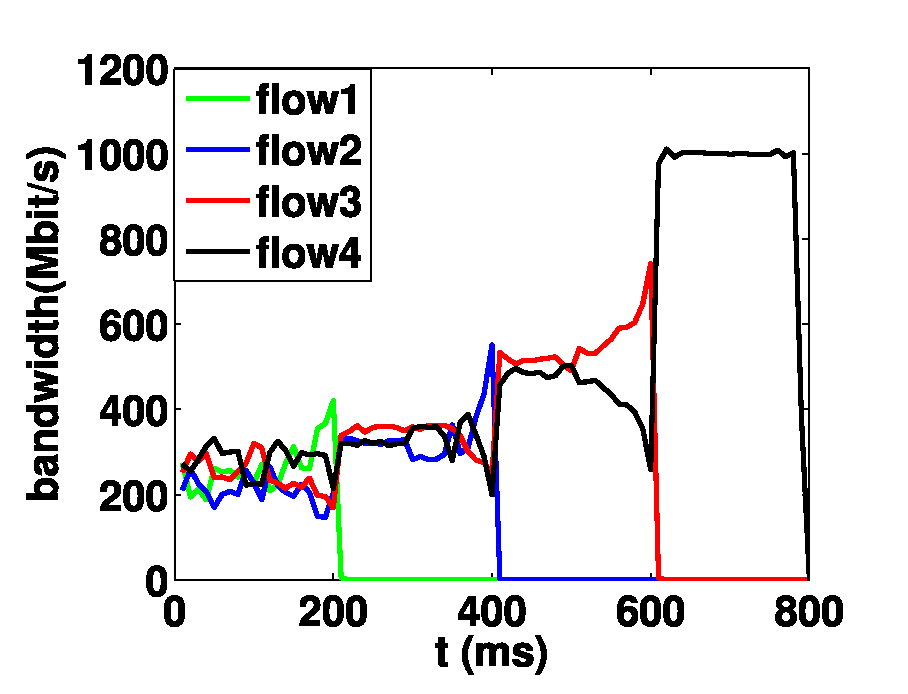
\includegraphics[width=0.5\columnwidth]{figures/LPD/bandwidth.eps}}%
  \subcaptionbox{拥塞窗口\label{LPD_Motivation:subfig2}}
      {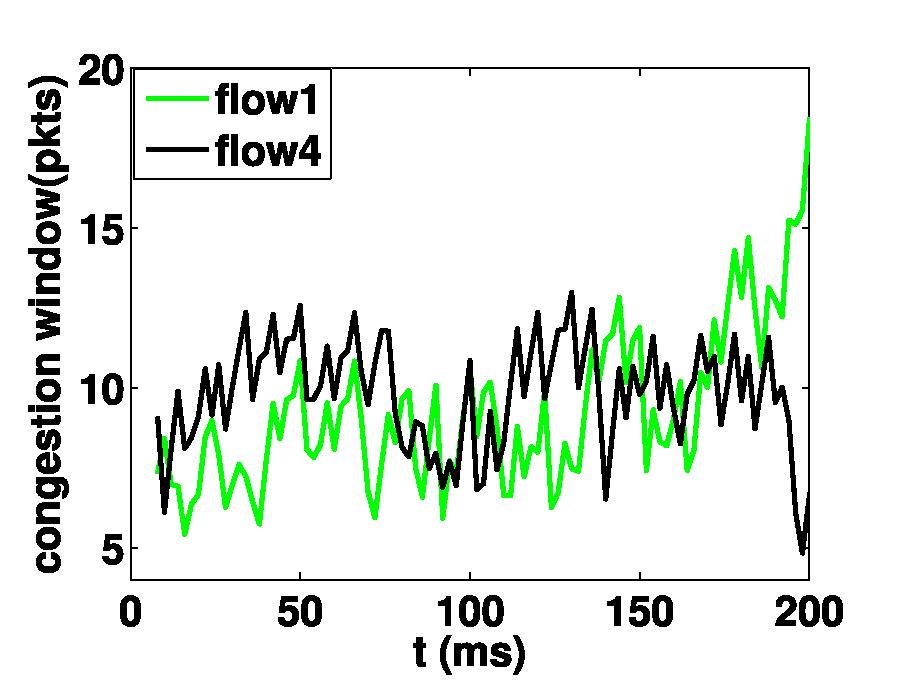
\includegraphics[width=0.5\columnwidth]{figures/LPD/cwnd.eps}}
  \subcaptionbox{flow$_1$和flow$_4$的期限因子\label{LPD_Motivation:subfig3}}%标题的长度,超过则会换行,如下一个小图。
    {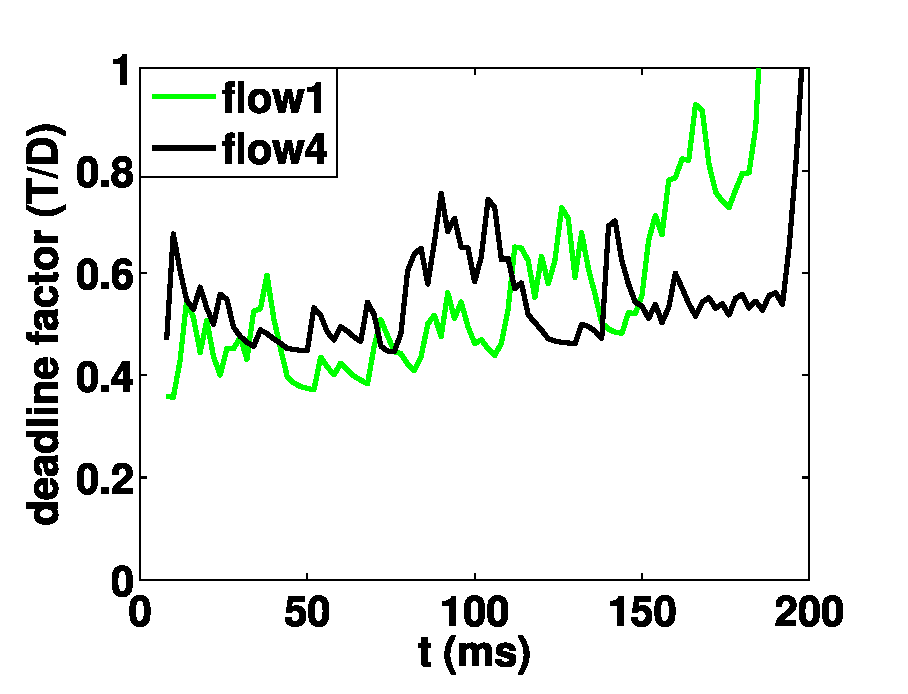
\includegraphics[width=0.5\columnwidth]{figures/LPD/deadlinefactor.eps}}%
  %\hspace{7em}%
  \subcaptionbox{flow$_1$和flow$_4$的拥塞因子\label{LPD_Motivation:subfig4}}
      {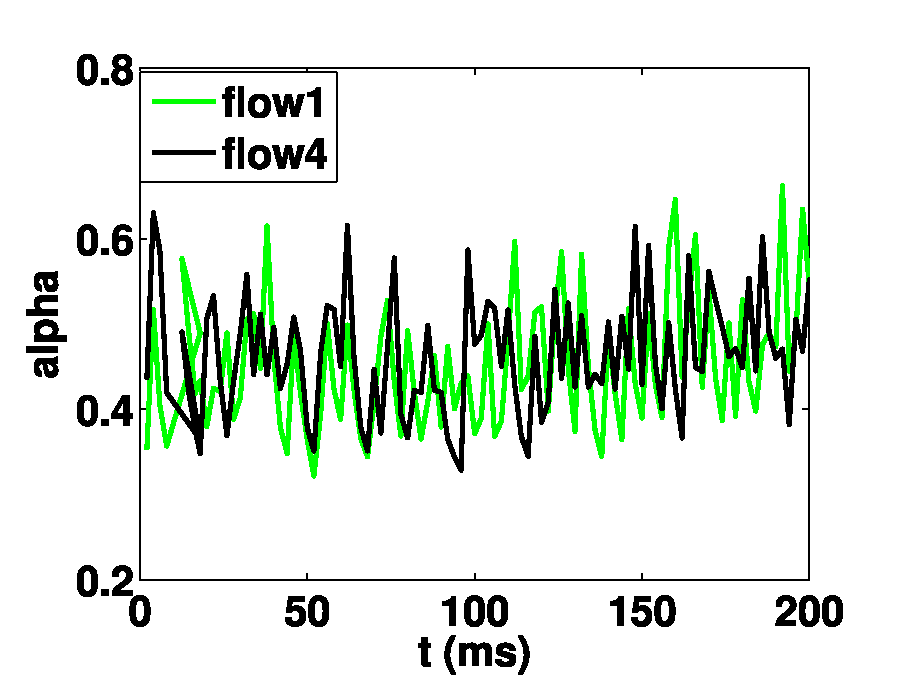
\includegraphics[width=0.5\columnwidth]{figures/LPD/alpha.eps}}
  \caption{D$^2$TCP的性能:4条并发流}
  \label{LPD_Motivation}
\end{figure}

\begin{figure}[h]
\centering
\subcaptionbox{$p=\alpha^d$\label{LPD_Gamma:subfig1}}
 {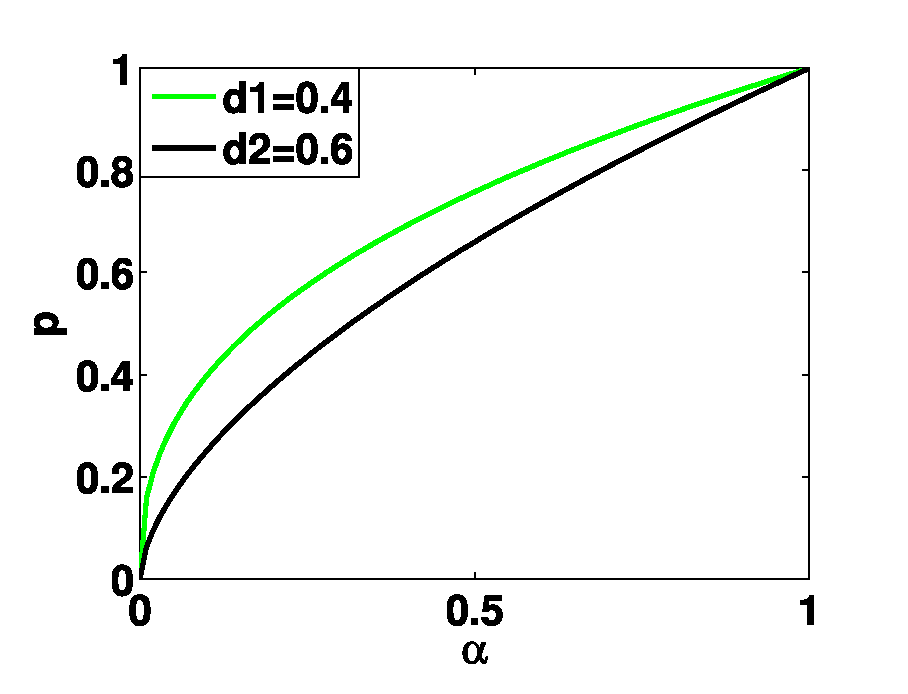
\includegraphics[width=0.45\columnwidth]{figures/LPD/gamma.eps}}
\subcaptionbox{$pd=p(\alpha, d_{1})-p(\alpha, d_{2})$\label{LPD_Gamma:subfig2}}
{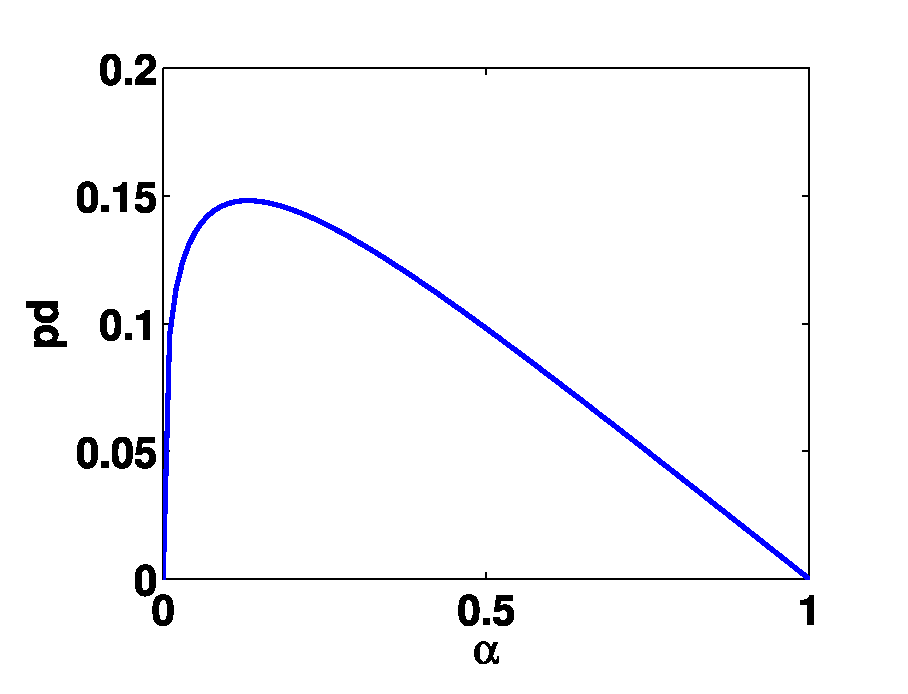
\includegraphics[width=0.45\columnwidth]{figures/LPD/PD.eps}}
\caption{D$^2$TCP 使用伽马校正函数来减小拥塞窗口}
\label{penalty-fig}
\end{figure}



为了验证D$^2$TCP存在的问题,本部分使用ns-2进行如下仿真:假设四条流通过瓶颈带宽为1Gbps链路,
流同时启动,大小分别为8,16,32和40 MB,截止期限分别为200,400,600和800 ms,
设置RTT为100 us。
如果使用TCP,那么可以使得所有流在最晚的截止期限(800ms)之前完成。
流传输结果如表\ref{flowtable}第四列所示,
表\ref{flowtable}中每个数字表示在流截止期限到达时剩余多少数据未被发送完成
(传输完成后,数据流会被强制停止)。
把非基于期限调整的策略DCTCP也放在最后进行比较。
从表\ref{flowtable}可以看到,尽管D$^2$TCP在流截止时间(deadline)之前传输的数据比DCTCP多,
但不能有效地减少错失期限流的数目。
在这两种情况下,只有flow$_4$在截止时间之前完成。
根据实验结果显示,在一些场景下,D$^2$TCP的性能和DCTCP的性能类似。 

图\ref{LPD_Motivation}显示了D$^2$TCP传输的更多细节,
D$^2$TCP使用w = w$\times$(1-$\alpha^d$/ 2)来调整其拥塞窗口w,
其中$\alpha$是估计的拥塞程度,d是期限迫近因子。
图\ref{LPD_Motivation}(a)描绘了flow$_1$和flow$_4$的带宽。
可以发现,大部分时间流之间带宽差别很小。
图\ref{LPD_Motivation}(b)是flow$_1$和flow$_4$在最初200ms期间的拥塞窗口大小,
除了快接近最后的10ms时,flow$_1$的窗口会比flow$_4$大很多之外,大部分时间,flow$_1$和flow$_4$的差距不大。
但是,图\ref{LPD_Motivation}(c)所示,flow$_1$和flow$_1$的期限迫近因子相差很大,
特别是在100 ms到200 ms的时间内。
为了完整性,图\ref{LPD_Motivation}(d)也绘制了$\alpha$,它表示flow$_1$和flow$_4$对拥塞程度的一种评估。
 
 
 \section{“越拥塞,越区分”的设计原则}
 \label{sec_LPD:MORE_LOAD}
 本章的工作主要借鉴DCN中较早的速率控制方案,如DCTCP,D$^2$TCP和L$^2$DCT等。
 特别是D$^2$TCP,通过将期限控制函数与DCTCP相结合,本质上给不同的数据流分配不同的带宽,
 从而相同条件下期限紧迫的流获得更多的带宽。
 正如\ref{sec_LPD:Motivation}节所示,本文认为仅仅通过期限对数据流进行带宽调整是不够的。 
 在\ref{sec_LPD:gamma}节中,本文分析出现这种不好的情况的根本原因。 
 在\ref{sec_LPD:principle}节,本文提出基于截止期限的速率控制策略的设计原则,
 并且使用数学语言对之进行描述。
 
\subsection{分析伽马校正函数}
\label{sec_LPD:gamma}

本部分对D$^2$TCP进行深入探究。
D$^2$TCP的核心思想是在惩罚函数中使用伽马校正函数p($\alpha$,d)=$\alpha^d$,其中0 <$\alpha$<1。
图 \ref{penalty-fig}(a)显示的是d = 0.4和d = 0.6时伽马校正函数的曲线。
可以发现,当$\alpha$增加时,p也增加,因此可以认为网络负载加重,拥塞窗口变小。
这个性质对于基于期限的速率控制确实是合理的和必要的。
然而,如果考虑惩罚函数的差异,
例如$pd(\alpha, d_{1}, d_{2})=p(\alpha, d_{1})-p(\alpha,d_{2})=\alpha^{d_{1}}-\alpha^{d_{2}}$,
其中$d_{1}$ <$d_{2}$,可以发现pd首先随$\alpha$的增加而增加,
在$\alpha$经过某一点(图\ref{penalty-fig}(b)中0.2左右)之后减小。
例如,pd(0.4,0.4,0.6)= 0.116,
pd(0.6,0.4,0.6)= 0.079,
而pd(0.9,0.4,0.6)= 0.019。
因而,网络拥塞程度较重的环境中,D$^2$TCP对期限不同数据流的调整能力基本失效,
变成一个公平分配方案,这不符合基于期限的拥塞控制策略的要求。
 
 
 解释D$^2$TCP在网络重度拥塞时失效的原因。
在150ms到160ms的时间间隔,$\alpha$从0.4增加到0.6,flow$_1$和flow$_4$的紧急因子分别是$d_1$ = 0.6和$d_4$ = 0.4,
因而flow$_1$比flow$_4$更紧急。
然而,pd(0.6,$d_4$,$d_1$)= 0.079,pd(0.4,$d_4$,$d_1$)= 0.116。 
如图\ref{LPD_Motivation}(b)所示,当网络拥塞程度变大时,
flow$_1$的窗口和flow$_4$的拥塞窗口大小基本相同(注意,pd(0.9,$d_4$,$d_1$)=0.019)。 
因而,flow$_1$在截止期限之前无法获得足够的带宽,从而无法在截止期限之前完成。
实际中,需要不同截止期限的流获得不同的带宽,从而流均在截止期限之前完成。


\subsection{基于截止期限的速率控制策略设计原则}
\label{sec_LPD:principle}

对于OLDI应用,由于查询流并发数目高,网络负载常常很大。
基于此,本文主张在设计基于截止期限的网络拥塞控制策略时应遵循以下原则:

(1)紧急原则(PI):截止期限近流获得的带宽应该高于截止期限远的流获得带宽。

(2)差异原则(PD):当网络负载变大时,截止期限不同的流获得的带宽的差异应该增加。 


PI表示数据流速率应该根据流的截止期限进行区分:考虑两条大小相同的数据流(长度一致),
截止期限近的流应该使用比截止期限远的流获得更多的带宽,
从而流在截止期限之前完成的概率会变大。
事实上,PI在新的基于TCP的拥塞控制方案(如$D^3$或D$^2$TCP)被采纳。
但是,当前基于TCP的拥塞控制方案,忽略了拥塞和数据流带宽差异之间的关系。



PD表示网络负载越重,流之间带宽差异性应该越大。
与网络负载较轻时相比,网络负载较重时,每条数据流获得的带宽都会减少。
从而,错失截止期限的可能性会变大。 
因此,为了尽可能的让数据流在截止期限之前完成,
期限近的流应从期限远的数据流抢夺带宽。
 
因此,截止期限不同的两条流获得带宽的差异性在拥塞程度大的情况下应该更大。
通过此方式,截止期限近的流和截止期限远的流都能在截止时间之前完成。
事实上,当前基于截止期限的拥塞控制策略忽略网络拥塞和期限的关系。
在形式上,假设r($\alpha$,d)表示在网络拥塞情形为$\alpha$(0 <$\alpha$<1),紧急因子为d(d> 0)的情形下流的带宽。
d越大表示期限因子越大,$\alpha$越大表示网络越拥塞。

定理\ref{theorem-principle}是对PI和PD的数学描述。

\begin{lemma}\label{theorem-principle}
 $r$ 遵守PI和PD的充分必要条件是 $\frac{\partial{r}}{\partial{d}}>0$, 
并且 $\frac{\partial^{2}{r}}{\partial{d}\partial{\alpha}}>=0$ 
(但是不能恒为0)

\end{lemma}


\begin{proof}
引理\ref{theorem-principle}中第一个式子表示PI:r是d的增函数。
说明期限因子越大,惩罚函数也越大,当出现拥塞时,滑动窗口减小的少。
下面证明说明第二个式子表示PD:
定义 $dr(\alpha, d_{1}, d_{2})=r(\alpha, d_{2})-r(\alpha, d_{1})$.
存在:
\begin{eqnarray}\label{eqn-partial}
\frac{\partial{dr(\alpha, d_{1}, d_{2})}}{\partial{\alpha}}
&=&\frac{\partial \left[r(\alpha, d_{2})-r(\alpha, d_{1}) \right]}{\partial{\alpha}} \nonumber \\
&=&\frac{\partial{r(\alpha, d_{2})}}{\partial{\alpha}} - 
\frac{\partial{r(\alpha, d_{1})}}{\partial{\alpha}}
\nonumber \\
&=& \int_{d_{1}}^{d_{2}}\!\!\frac{\partial^{2}{r}}{\partial{\alpha}\partial{d}} \,\,\mathrm{d}d.
\end{eqnarray}

考虑PD的数学意义,PD等价于: 
$dr(\alpha_{2}, d_{1}, d_{2})>dr(\alpha_{1}, d_{1}, d_{2})$
, $\alpha_{1}<\alpha_{2}$ 并且 $d_{1}<d_{2}$ 时成立, 
根据 (\ref{eqn-partial}),
当且仅当
$\frac{\partial{dr(\alpha, d_{1}, d_{2})}}{\partial{\alpha}}>0$
,$d_{1} < d_{2}$成立
, 如果有
$\frac{\partial^{2}{r}}{\partial{\alpha}\partial{d}} \ge 0$ (但是不能恒为0)
\end{proof}

上面提出的原则简单并且有通用型,
而在使用中,如何设置流的截止期限,
以及如何设计由$\alpha$和d作为参数的惩罚函数,可以根据具体的应用来确定。 
在下一小节中,本文将根据这个原则开发一个具体的根据截止期限和网络拥塞函数进行拥塞控制的策略-正比负载差分策略。

\section{正比负载差分策略(LPD)以及分析}
\label{sec_LPD:LPD}

\subsection{正比负载差分策略(LPD)}
作为”越拥塞,越区分”原则的一个应用,我们提出了下面的基于期限的拥塞控制算法:
\begin{equation}
w=
\begin{cases}
w+(1-f) &\text{没有拥塞}\\
w \times (1-f) &\text{出现拥塞}
\end{cases}
\label{LPD-CA-eq}
\end{equation}


其中f=$\alpha$/d是惩罚函数,
这个函数是根据网络负载$\alpha$和紧急因子d进行计算的,
这个因子可以用来区分流的紧急程度。
拥塞程度(即网络拥塞负载因子$\alpha$)的含义和DCTCP以及D$^2$TCP中的相同\cite{DCTCP, D2TCP}。 
由于f与$\alpha$成正比,所以我们称这个算法为正比负载差分策略(Load Proportional Differentiation,简称LPD )。 

定义一个简单的迫近因子d = $t_{max}/t$,
其中t是流开始时间时刻和截止时刻之间的持续时间,
$t_{max}$是t的可调上界,后面会有详细讨论。
对于没有截至期限的流,t可以设置为$t_{max}$。 
可见,t越小,d越大,因此流也越迫切。
基于此,可以得到LPD-t,一个根据网络拥塞和截止期限进行拥塞控制的策略:

\begin{equation}
w=
\begin{cases}
w+(1-\alpha \times \frac{t}{t_{max}}) &\text{没有拥塞;}\\
w \times (1-\alpha \times \frac{t}{t_{max}}) &\text{出现拥塞}
\end{cases}
\label{LPD-t-eq}
\end{equation}


根据(\ref{LPD-t-eq})我们可以看到LPD-t是一个简单策略:
首先计算惩罚函数$f=\alpha \times \frac{t}{t_{max}}$ ,
根据f的值来调控拥塞窗口。
如果网络中没有拥塞,那么拥塞窗口每个RTT增加$(1-f)$,
如果发生拥塞,那么拥塞窗口减小f倍。
 
\subsection{LPD分析}

\subsubsection{LPD简单分析}
在类似TCP的方案中,通过调整拥塞窗口来间接的调整流的发送速率。
因此,我们可以通过调整拥塞窗口的大小来调整发送速率。
LPD-t是符合我们提出“越拥塞,越区分”的设计原则的,
引理\ref{theorem-LPD}对此进行了证明。
 
\begin{lemma}\label{theorem-LPD}
LPD 服从 PI 和 PD. 
\end{lemma}
\begin{proof}
$\frac{\partial{(1-f)}}{\partial{d}}
=\frac{\partial{(1-\alpha/d)}}{\partial{d}}
=\frac{\alpha}{d^{2}}>0$, 
并且
$\frac{\partial^{2}{(1-f)}}{\partial{d}\partial{\alpha}}
=\frac{1}{d^{2}}>0$, 
因此LPD-t窗口的限制,满足引理 \ref{theorem-principle}, 
因此LPD-t满足 PI 和 PD。
\end{proof}

从几何角度来看LPD遵循PI和PD这两个原则。 
由于f与$\alpha$成正比,
所以($\alpha$,f)的几何表示是一条穿过原点的直线,窗口变化服从线性规则。
如果两条流有不同的期限因子d,那么两条数据流的惩罚函数f之间的差会随着$\alpha$的增大而增加。
引理\ref{theorem-LPD_2}展示在两条流的场景下,
LPD-t稳定速率与期限成反比。


\begin{lemma}\label{theorem-LPD_2}
假设LPD-t可以使流收敛在一个稳定的状态,
即拥塞窗口在一个固定的区间内稳定的波动,
此时流有稳定的发送速率,并且计算出的拥塞程度趋于稳定状态。 
如果$t\ll t_{max}$,其中t和$t_{max}$是在(\ref{LPD-t-eq})中LPD-t使用的调整$t_{max}$参数。
那么近似地,流达到的稳定速率与之对应的期限成反比。
\end{lemma}


\begin{proof}
在稳定状态中,流的拥塞窗口变化规律是固定周期为$N$的锯齿形。 
使用 $W_{min}$ 和 $W_{max}$来代表一个周期内的最小和最大窗口,我们有:

$W_{max}=W_{min}+N \times (1-\alpha \times \frac{t}{t_{max}})$, 
并且 $W_{min}=W_{max} \times (1- \alpha \times \frac{t}{t_{max}})$, 
根据上面,我们有
$W_{max}= N \times (1-\alpha \times \frac{t}{t_{max}})/(\alpha \times \frac{t}{t_{max}})$, 
并且平均窗口大小为: $W_{av}= (1- \alpha \times \frac{t}{2t_{max}}) \times W_{max}$。

对于两条流,$f_{1}$ 和 $f_{2}$。
两条流的持续时间为 $t_{1}$ 和 $t_{2}$, 
假设两条流的最大窗口是$W_{1}$ 和 $W_{2}$, 
流稳定的发送速率为 $r_{1}$ 和 $r_{2}$, 
 两条流的速率比例,$\frac{r_{1}}{r_{2}}$ 可以计算如下:
\begin{eqnarray}
\frac{r_{1}}{r_{2}} &=& \frac{(1-\alpha \times \frac{t_{1}}{2t_{max}}) \times W_{1}}{(1-\alpha \times \frac{t_{2}}{2t_{max}}) \times W_{2}} \nonumber \\
&=& \frac{t_{2}}{t_{1}} \times \frac{2t_{max}-\alpha \times t_{1}}{2t_{max}-\alpha \times t_{2}} \times \frac{t_{max}-\alpha \times t_{1}}{t_{max}-\alpha \times t_{2}} \nonumber
\end{eqnarray}
如果$t \ll t_{max}$, 然后 $r_{1}/r_{2} \approx t_{2}/t_{1}$.
\end{proof}

\begin{figure}[h]
\centering
\subcaptionbox{单条流的带宽}
 {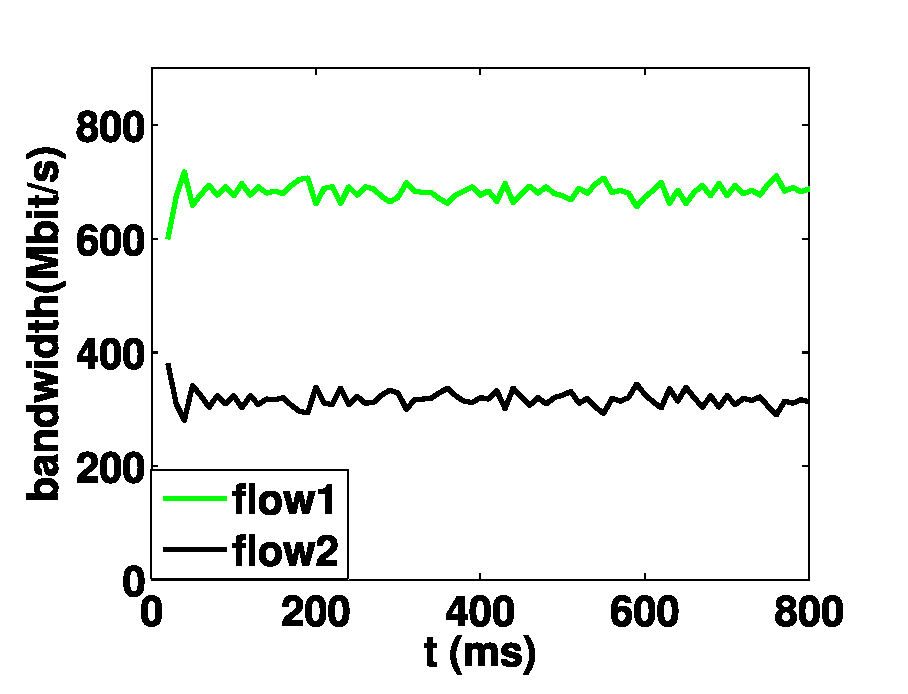
\includegraphics[width=0.45\columnwidth]{figures/LPD/rate2.eps}}
\subcaptionbox{$pd=p(\alpha, d_{1})-p(\alpha, d_{2})$}
{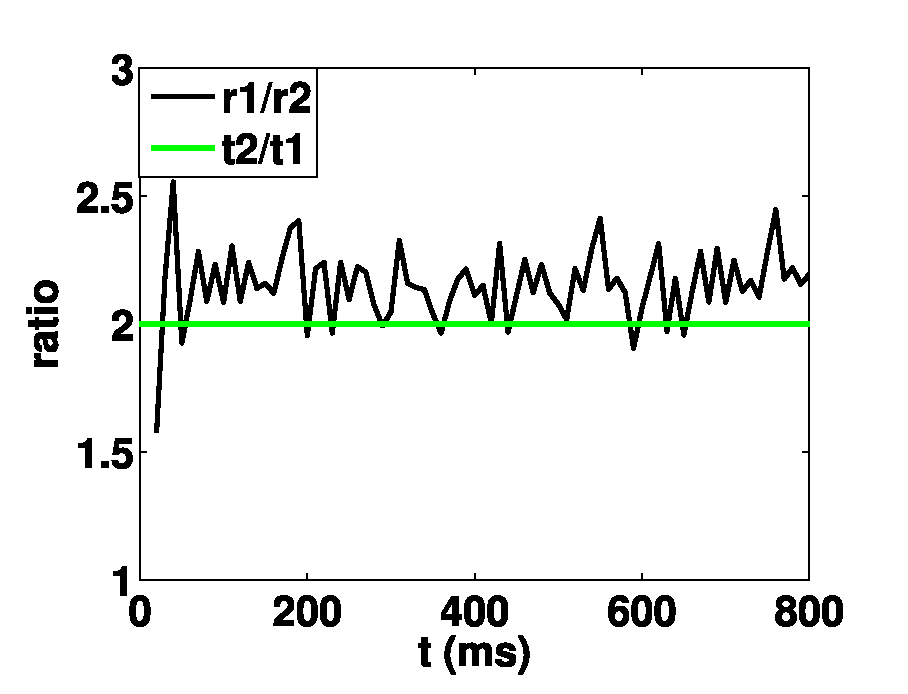
\includegraphics[width=0.45\columnwidth]{figures/LPD/ratio.eps}}
\caption{LPD下的两条流}
\label{rate-analysis-fig}
\end{figure}

尽管LPD-t的稳定性还没有得到证实。
实际上,流截止期限不能比$t_{max}$小得多,为了验证引理\ref{theorem-LPD_2},进行以下验证: 
启动两条均为100 MB的LPD-t长流,两条流的截止时间为$t_1$ = 5s,$t_2$ = 10s,设置$t_{max}$ = 50s。 
图\ref{rate-analysis-fig}(a)描述了前800 ms流的带宽变化过程,
可以看到,flow$_1$的带宽平均是670M/s,而flow$_2$的带宽平均是330M/s。
图\ref{rate-analysis-fig}(b)描述了两条数据流实际带宽比率,可以发现$r_1/r_2 \approx t_2 / t_1$=2。


\subsubsection{LPD流模型}
假设N个并发的流通过容量为C pkts / sec的瓶颈链路传递给同一个接收者节点。
设置(\ref{Model-CA-eq})中$f_1(\alpha)=f_2(\alpha)=\alpha \times \frac{t}{t_{max}}$,
同时把$f_1(\alpha)$和$f_2(\alpha)$带入(\ref{fluid-model_window})$\sim$(\ref{fluid-model-q}),
并且改动(\ref{Model-alpha-eq})中数据包标记的方法,并且增加$\alpha$标记方法,那么LPD流模型可以描述为:


 \begin{align}
&\frac{dw_i}{dt}=\frac{1-\alpha_i(t)\frac{t_i}{t_{max}}}{R(t)}-\frac{w_i(t)\alpha_i(t)\frac{t_i}{t_{max}}}{R(t)}p(t-R^*)  \label{LPD-model_window} \\
&\frac{d\alpha_i}{dt}=\frac{g}{R(t)}(p(t-R^*)-\alpha_i(t)) \label{LPD-model_alpha} \\
&\frac{dq}{dt}= \sum_{i=1}^N{\frac{w_i(t)}{R(t)}}-C \label{LPD-model_queue}  \\
&\widehat{p}(t)=1_{\widehat{q}(t)>1}  \label{LPD-model_mark}
\end{align}



其中,$w_i$表示$flow_i$的拥塞窗口的大小。 
$t_i$是$flow_i$的截止期限,$\alpha_i$表示$flow_i$的拥塞程度。 
q是交换队列长度,R表示RTT。
公式 (\ref{LPD-model_alpha}) 和 (\ref{LPD-model_mark})描述了交换机的ECN标记过程。
(\ref{LPD-model_window}) 模拟的是拥塞窗口。
公式(\ref{LPD-model_queue})描述交换机队列长度。
利用该模型,可以推算出窗口大小和队列长度。

\begin{figure}[h]
\centering
\subcaptionbox{窗口大小}
 {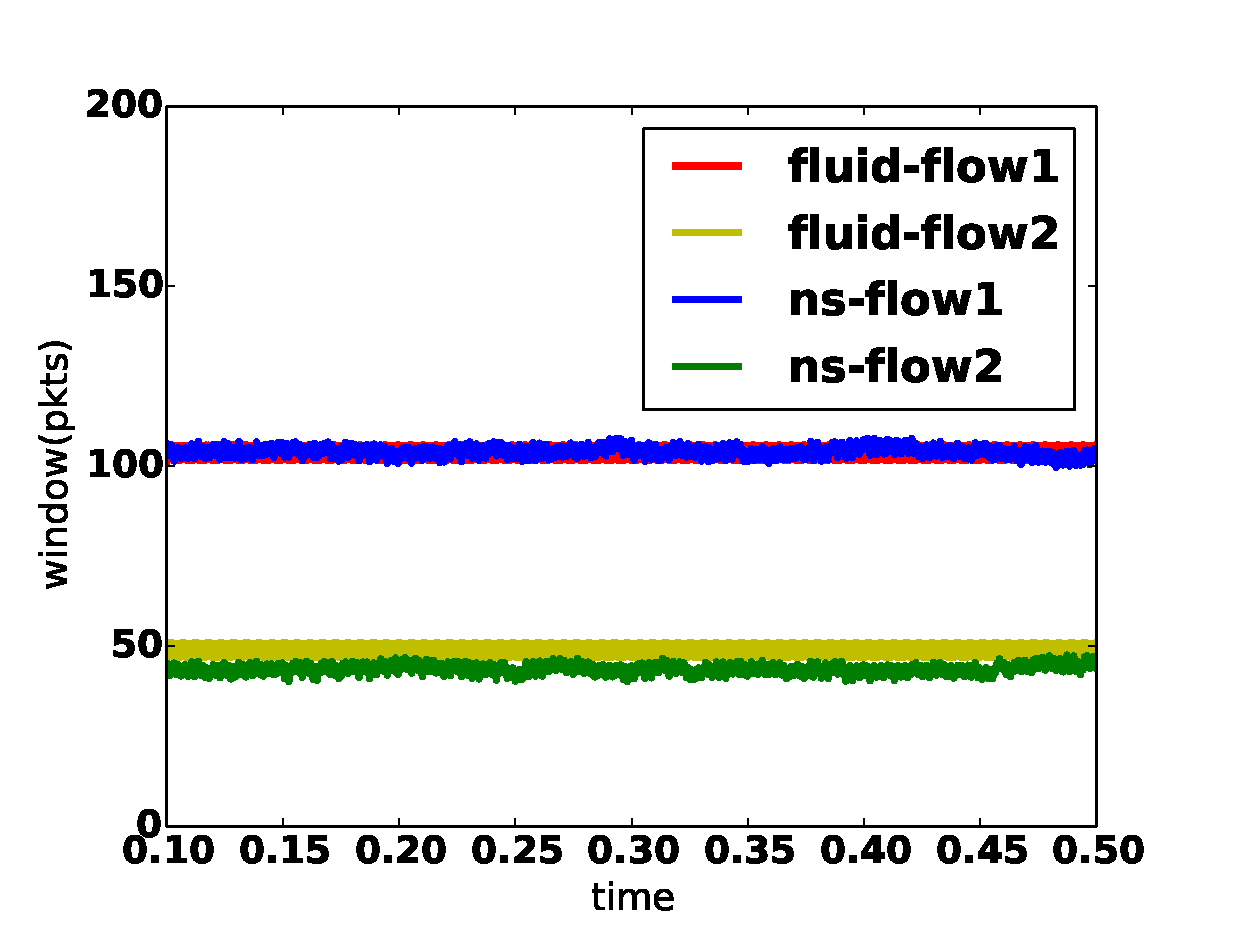
\includegraphics[width=0.32\columnwidth]{figures/LPD/2/window.eps}}
\subcaptionbox{队列长度}
{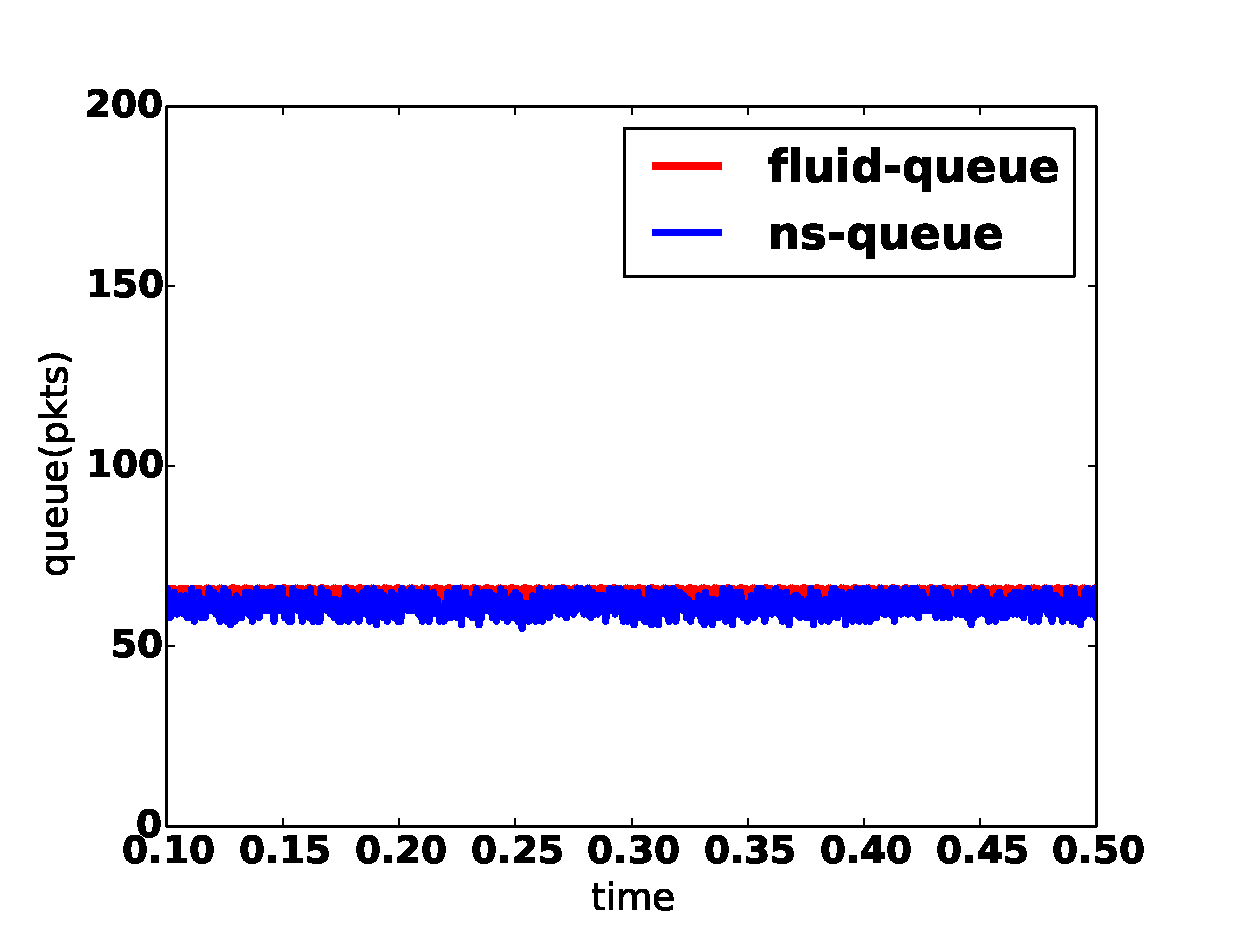
\includegraphics[width=0.32\columnwidth]{figures/LPD/2/queue.eps}}
\subcaptionbox{$\alpha$}
{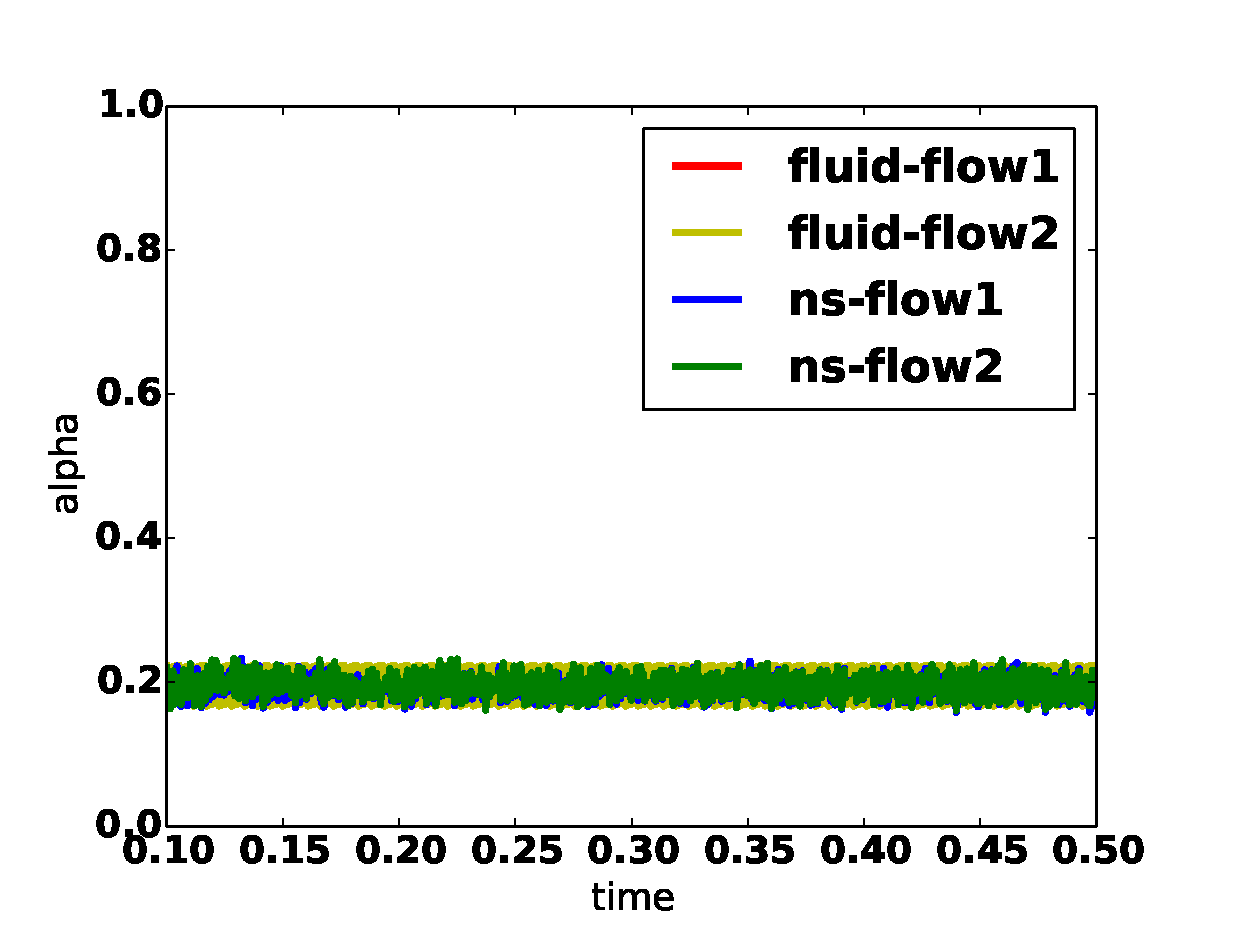
\includegraphics[width=0.32\columnwidth]{figures/LPD/2/alpha.eps}}
\caption{LPD 流模型和ns-2下结果对比}
\label{rate-analysis-fig}
\end{figure}


为了验证模型,启动两条长流,
期限分别是$t_1$ = 10s,$t_2$ = 20s,同时设置$t_{max}$ = 40s。
使用相同的参数在ns-2和流体模型下对比窗口大小,队列长度和拥塞程度。
窗口大小,队列长度和拥塞程度的仿真结果与模拟结果对比分别如图\ref{rate-analysis-fig}(a),
图\ref{rate-analysis-fig}(b)和图\ref{rate-analysis-fig}(c)所示。
可以看到使用流模型的推算结果和ns-2的模拟结果基本相符。



\begin{figure}[h]
\centering
\subcaptionbox{单条流的带宽}
 {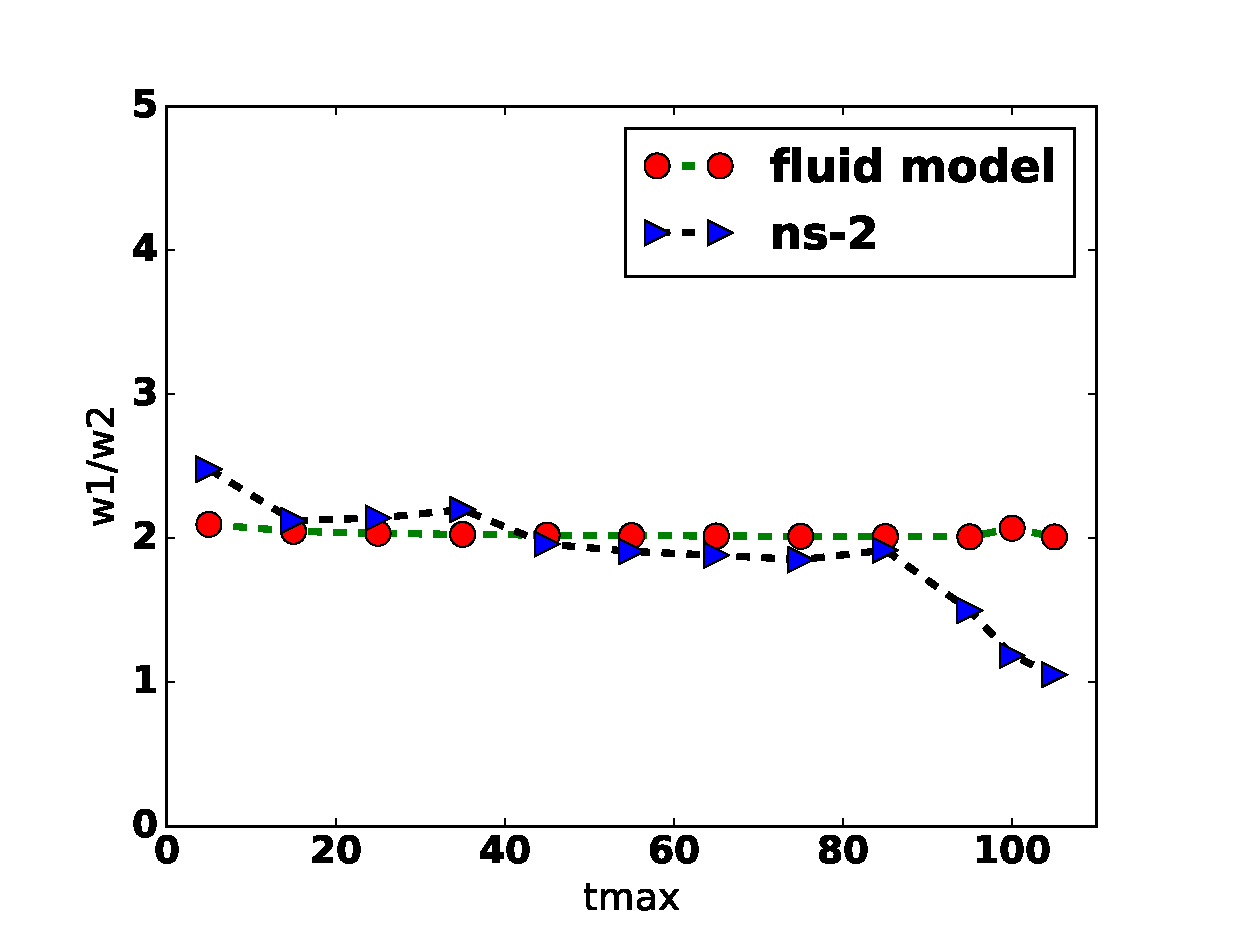
\includegraphics[width=0.45\columnwidth]{figures/LPD/parameter/ratio.eps}}
\subcaptionbox{$pd=p(\alpha, d_{1})-p(\alpha, d_{2})$}
{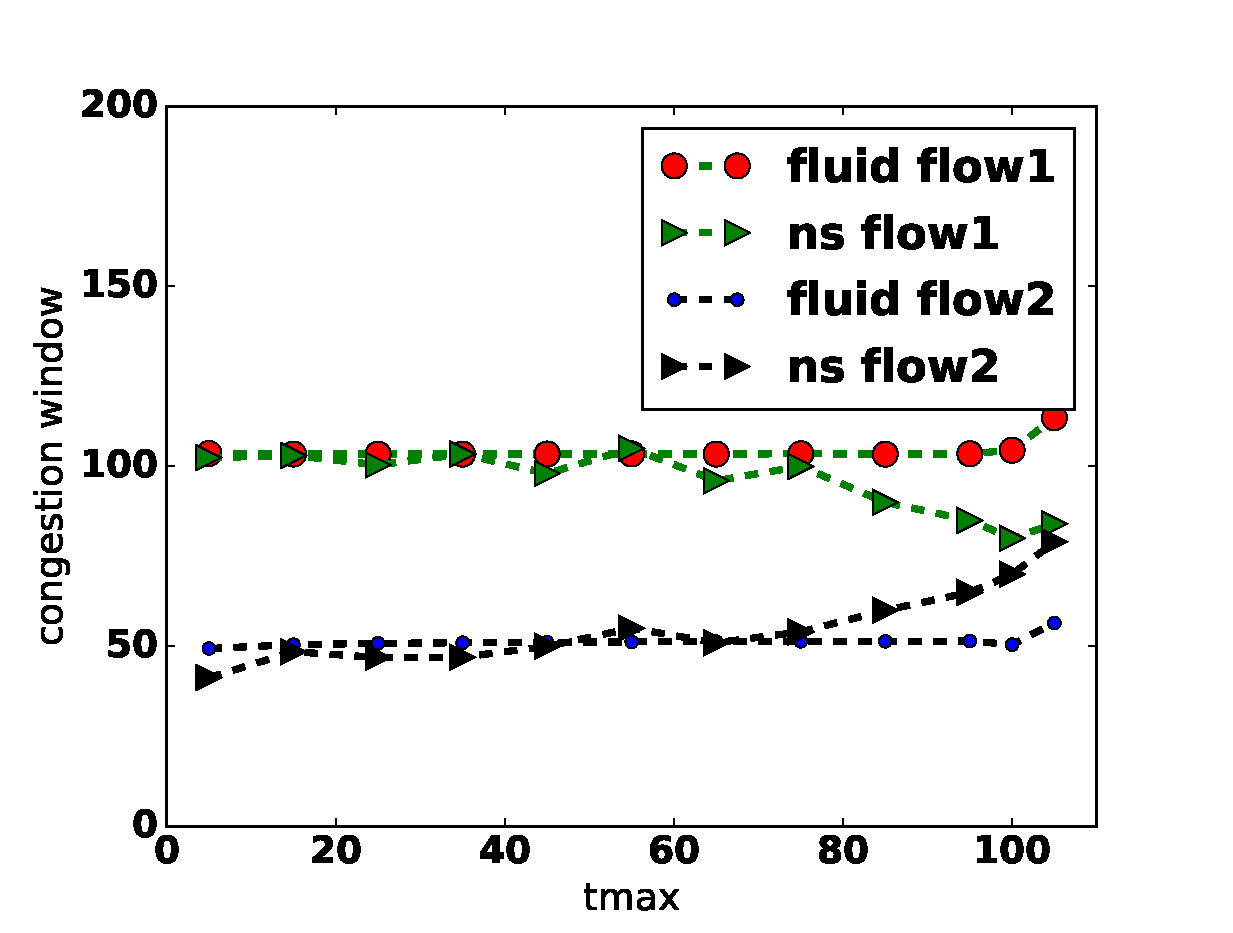
\includegraphics[width=0.45\columnwidth]{figures/LPD/parameter/window2.eps}}
\caption{LPD-t下的两条流}
\label{rate-ratio-fig}
\end{figure}



为了进一步测试模型的准确性,
启动两条长流,设置瓶颈带宽是10Gbps,两条流的期限分别是$t_1$ = 0.5 s,$t_2$ = 1s。
设置数据包大小为1500B,RTT为100 us,K为64。
图\ref{rate-ratio-fig}显示了模拟结果和ns-2方针结果的对比。
从图\ref{rate-ratio-fig}(a)可以看出,当$t_{max} <100$时,流模型和ns-2仿真的结果都是$w_1 /w_2 \approx 2$。
然而,当$t_{max}> 100$时,ns-2模拟的$w_1\approx w_2$和流模型的$w_1 /w_2 \approx  2$。
图\ref{rate-ratio-fig}(b)表明当$t_{max}> 100$时,流模型会推算出较大的拥塞窗口。
此表明,$t_{max}$在实际中应该被设置适当值,如何$t_{max}$,本章后续会进行更详细的讨论。



\subsubsection{$t_{max}$的选择}
注意,在LPD流模型中,流具有不动点$(w_i,\alpha_i)=(t_{max}-t_i,1)$。
不动点的实际意义是所有数据流的$\alpha= 1$。
即重度拥塞的情形下,所有的数据包都被标记,所有流拥有固定的拥塞窗口。
在LPD中,$t_{max}$应该选择适当的值。
下面分析$t_{max}$取值:

假设有N条流$(t_{max}> t_1> t_2> ...> t_n)$同时启动,
其中,$t_1$$\sim$$t_n$是流flow$_1$$\sim$flow$_n$的截止期限。
在时刻t,队列长度表示为q(t),则有:

\begin{equation}
\label{tmaxprocess}
\frac{t_{max}-t_1}{t_1}+\frac{t_{max}-t_2}{t_2}+...+\frac{t_{max}-t_n}{t_n} <q(t)+C\times RTT
\end{equation}



假设当交换机队列超过K时,数据包开始标记。
那么,对于N条数据流,每个RTT,拥塞窗口大小不超过1。
那么我们有$q(t) < K+N$。因为我们假设$t_{max}>t_1>t_2>…>t_n$,因此有:


\begin{equation}
\label{tmax}
t_{max}<\frac{t_1\times(K+C\times RTT+2N)}{N}
\end{equation}

根据(\ref{tmax}),我们可以根据截止期限的最大值,最大并发流量数量,
RTT和瓶颈链路链接带宽来设置$t_{max}$。 
在当前数据中心,设置C为10Gbps,数据包大小为1500B,RTT为100us,
因为数据中心,大多数情况下并发连接数小于100 \cite{DCTCP},假设设置K为60:


 \begin{equation}
\label{tmax_suggest}
t_1< t_{max}<3.5\times t_1
\end{equation}

在实际部署LPD时,可以根据(\ref{tmax})计算$t_{max}$。(\ref{tmax_suggest})可以当作 $t_{max}$的缺省值。
事实上,结果与图\ref{rate-ratio-fig} (b)一致。 
根据(\ref{tmax_suggest}),当$N = 2$时,$t_{max}\le76* t_1$。
在此情况下,$t_1 = 1s$, 从ns-2仿真中可以看出,当$t_{max}> 80$时,流拥塞窗口不再与其对应的t成反比。

\subsubsection{K的设置}
实际中,交换机的阈值K不可设置的过大或者过小,否则,链路利用率会很低。
在实际部署LPD时,需要使链路利用率达到$100\%$。
因此需要确定阈值K的设置范围\cite{DCTCPAnalysis}。

qmin,qmax表示交换机队列的最小和最大长度。
基于ECN标记的拥塞控制策略,队列长度在固定区间内波动。
阈值K应大于下冲振荡(否则队列大小将为零,链路利用率将不是$100\%$)。 
使用LPD流模型,并将流的期限设置在10以内,将$t_{max}$从10变为55,
并将链路带宽从1Gbps变为10Gbps。 
最后,针对每一个$t_{max}$我们记下每组队列下限的最小值。
结果如图\ref{qmin-fig}所示。
可以看到g值很小,即使是最坏的情形($t_{max} = 55$, $t_{max}\simeq 5 t_1$),也可以得到:
\begin{equation}
\label{KRANGE}
K \gtrapprox0.4 CR
\end{equation}


\begin{figure}
\begin{minipage}{0.5\textwidth}
  \centering
  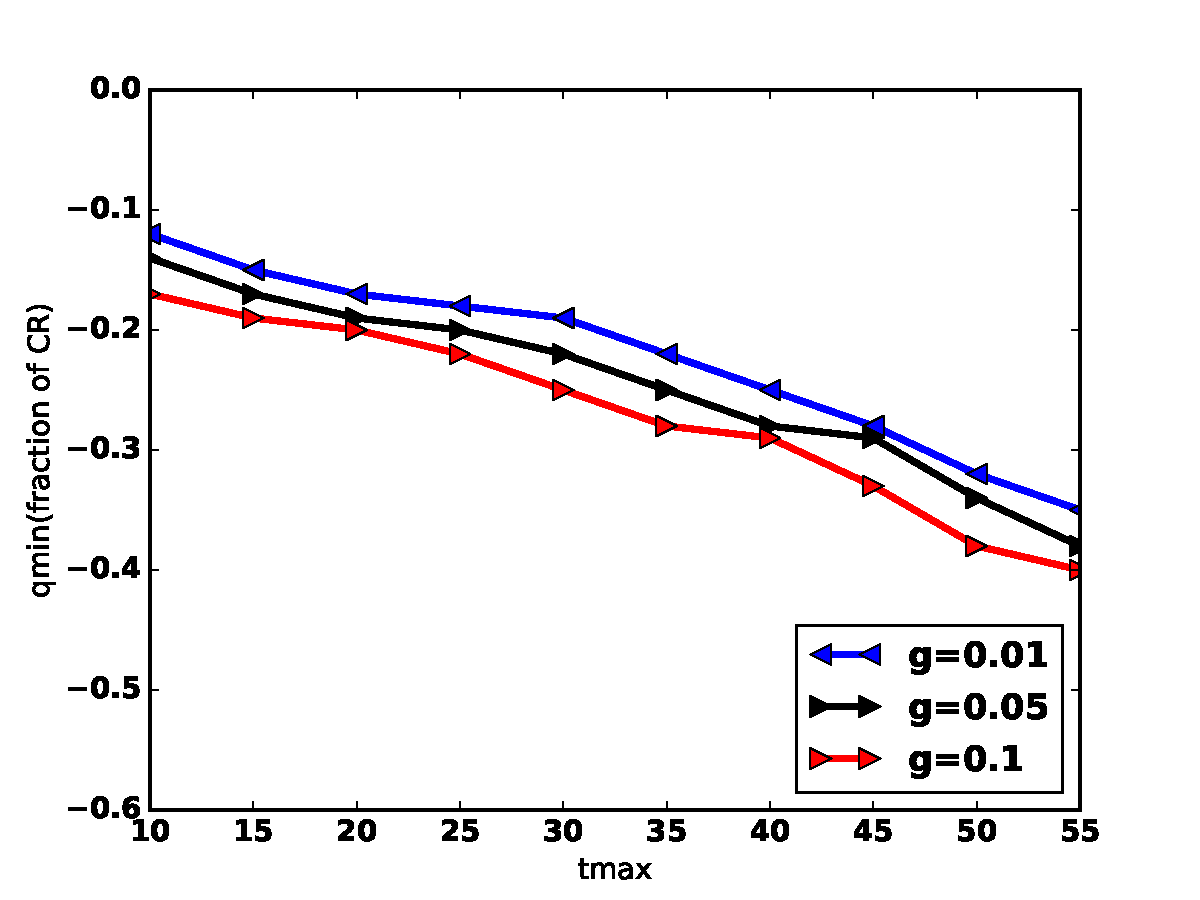
\includegraphics[width=0.7\columnwidth]{figures/LPD/model/qmin.pdf}
  \caption{队列最小长度波动}
  \label{qmin-fig}
\end{minipage}
\begin{minipage}{0.5\textwidth}
  \centering
  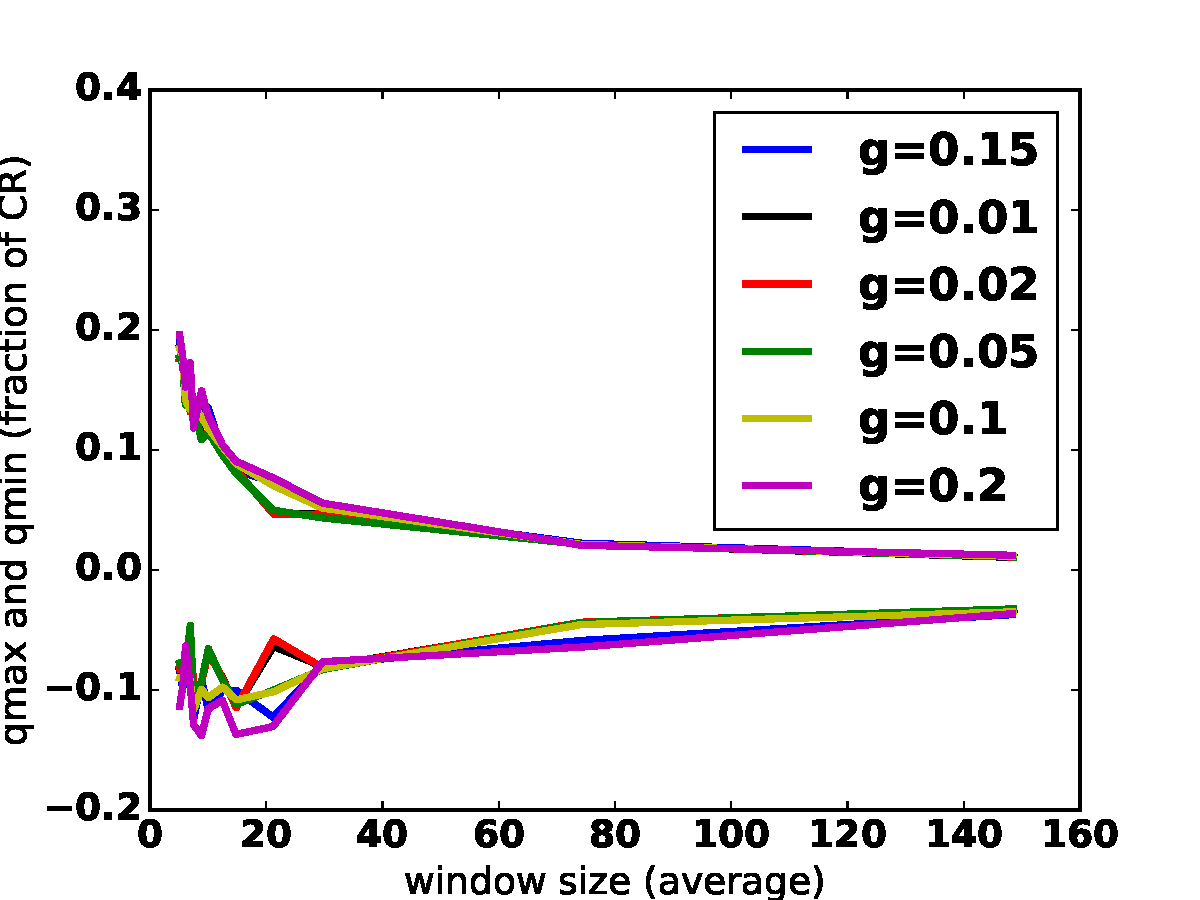
\includegraphics[width=0.7\columnwidth]{figures/LPD/model/k.pdf}
  \caption{队列最大和最小}
  \label{k-fig}
\end{minipage}
\end{figure}

\begin{figure}[H] 
  \centering
  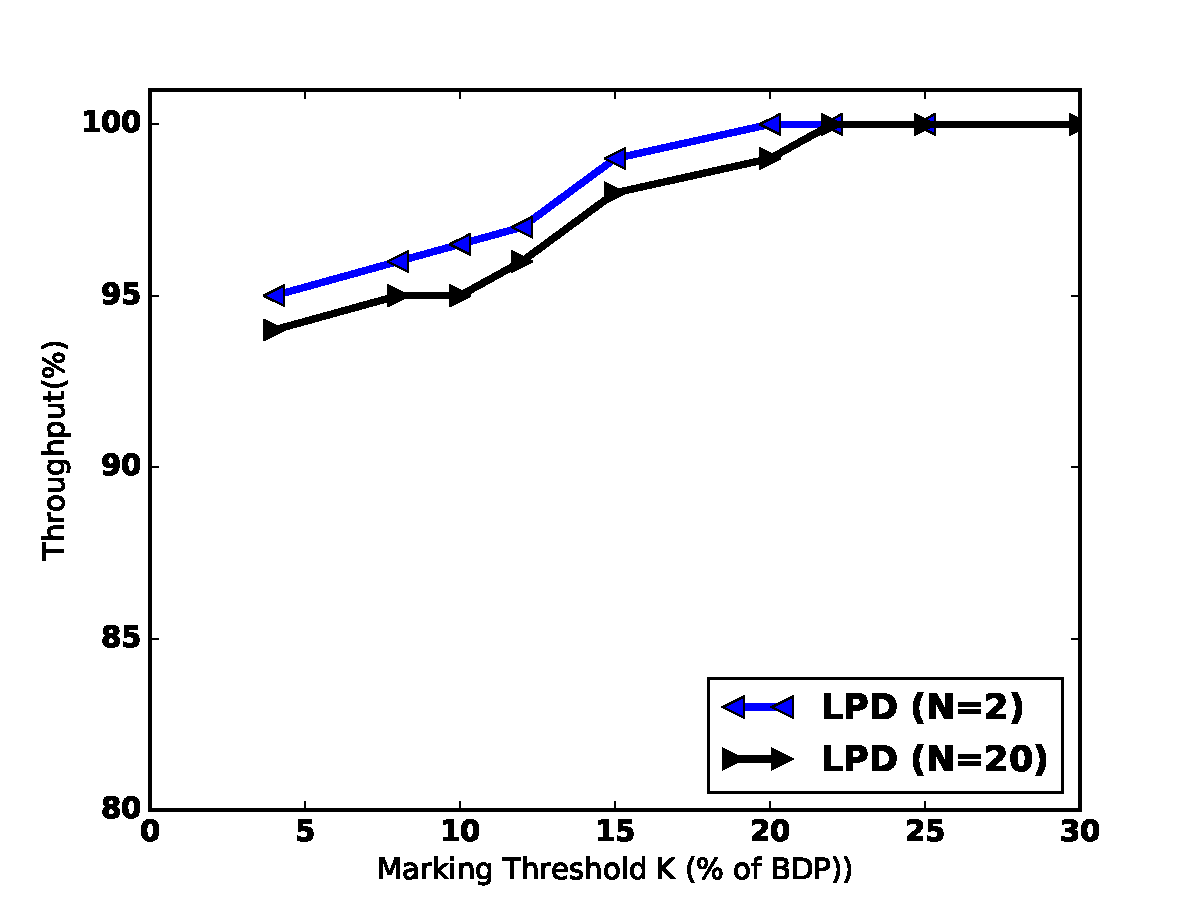
\includegraphics[width=0.6\columnwidth]{figures/LPD/model/throughput.pdf}
  \caption{ns-2仿真中吞吐量和标记阈值K的关系。从4到30个包(BDP的$2.4-18\%$)变化。 
结果表明,即使对于小于BDP的$3\%$的K,吞吐量仍然高于$95\%$}
  \label{throughput-fig}
\end{figure}


至于RTT,因为$R = d + K / C$,将R带入(\ref{KRANGE}),
所以在最坏的场景下,得到队列的缺省值0.67Cd。 
假设链路带宽是C =10Gbps,链路传送延迟d=100us,数据包大小是1500B,则K至少应该设置为56。
对于数据中心中常见的情形,链路传播延迟为100us,链路的瓶颈带宽为10Gbps。
设置$t_{max} = 10$,截止期限在1到10范围内随机生成。
使用LPD流模型,图\ref{k-fig}显示了flow$_1$,使用不同的g值下平均窗口大小与qmin和qmax(其中qmin表示队列最小值,qmax表示队列最大值,qmin和qmax换算成CR)的关系图。
可以看到$K\gtrapprox0.12CR$。
为了避免队列下溢,需要有$K > |qmin |C*R \simeq0.12CR$。  
由于$R=d+K/C$,因此可以得到:
\begin{equation}
\label{KVALUE}
K \simeq 0.14 Cd
\end{equation}

换言之,大约需要$14\%$的BDP就能实现链路利用率达到$100\%$。 
多余的缓冲区可以用来处理突发流。
为了测试上面的实验结果,图\ref{throughput-fig}显示ns-2仿真中吞吐量和标记阈值K的关系图。 
在这个实验中,变换K的取值从4到30(大约是BDP的$2.4\% \sim18\%$)。 
结果表明,ns-2仿真结果与LPD流模型相似,即使当K设置小于$3\%$倍的BDP时,吞吐量仍然高于$95\%$。 


\subsection{LPD拓展}
对期限敏感的OLDI应用常为小的查询流设置期限。
为了满足OLDI应用中有期限数据流的需求,
我们扩展LPD-t,并将流的大小考虑进去。
\begin{equation}\label{LPD-e-eq}
f=\alpha \times \frac{t}{t_{max}} \times \frac{s}{s_{max}}
\end{equation}
其中,$s_{max}$是流大小的上界。
这样,在链路带宽不足的场景下,小的数据流能获取更多的带宽,从而在截止时间(deadline)之前完成。
 (\ref{LPD-e-eq})仍然保留了LPD的特性,称此为LPD-e。 
 在本文后面的实验中,默认使用LPD-e,如果本文使用其他的策略,将会有明确说明。
 可以注意到“越拥塞,越区分”的原则是通用的,因此可以使用其他的形式。
本文选择仅仅因简单性而提出LPD,并将在后面中讨论一些其他形式的拥塞控制策略,其它形式的策略也满足此原则。
 另一方面,LPD本身也可以使用剩余流大小进行拓展。
 
\section{实验验证}\label{LPDevaluation}
本节通过ns-2 \cite{ns2}仿真和实际测试床来评估LPD的性能。 
本文根据DCTCP网站\cite{DCTCPcode}发布的DCTCP的源代码实现了LPD(包括LPD-t,LPD-e),
并将Vamanan\cite{D2TCP}提供的D$^2$TCP的ns-3代码移植到ns-2。 
另外,本文的实验同时实现L$^2$DCT,Karuna,并改动pFabric的代码到ns-2平台上。 
本文所有代码均可以在LPD开源代码网站\cite{LPD-sim-code}下载。 
同时本文的实验也在Linux内核3.2.61中实现了LPD,D$^2$TCP,L$^2$DCT,
并在真实环境上作评估,相应的源代码可以在LPD内核代码网站\cite{LPD-code}下载。

\subsection{解决研究动机提出的问题}

\begin{figure}[h]
  \centering%
  \subcaptionbox{流的带宽\label{LPD_Evaluation_Motivation:subfig1}} %标题的长度,超过则会换行,如下一个小图。
    {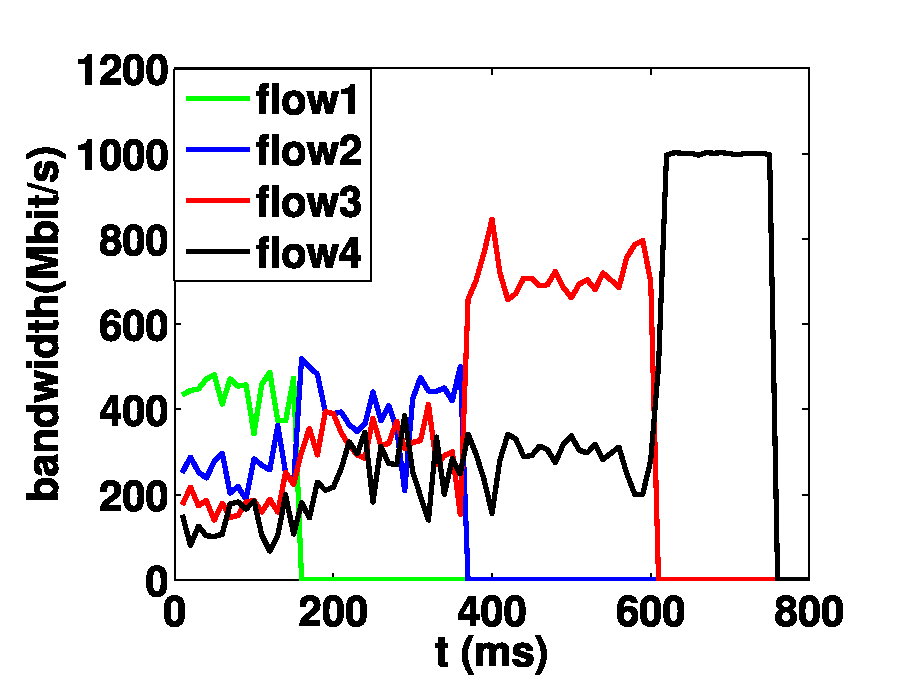
\includegraphics[width=0.5\columnwidth]{figures/LPD/evaluation_1/LPD_bandwidth2.eps}}%
  \subcaptionbox{拥塞窗口\label{LPD_Evaluation_Motivation:subfig2}}
      {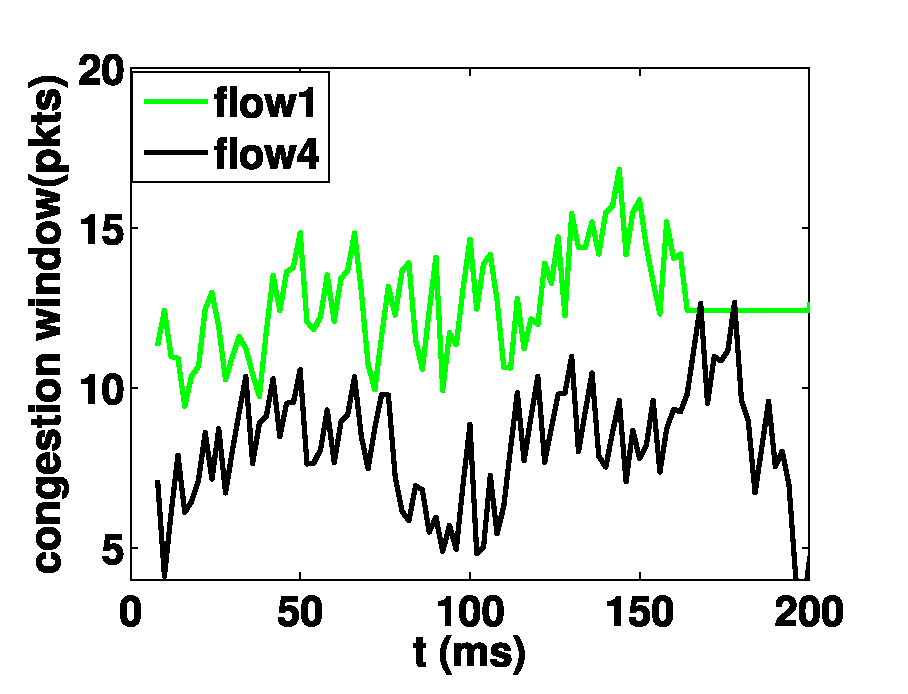
\includegraphics[width=0.5\columnwidth]{figures/LPD/evaluation_1/LPD_window2.eps}}
  \subcaptionbox{flow$_1$和flow$_4$的期限因子\label{LPD_Evaluation_Motivation:subfig3}}%标题的长度,超过则会换行,如下一个小图。
    {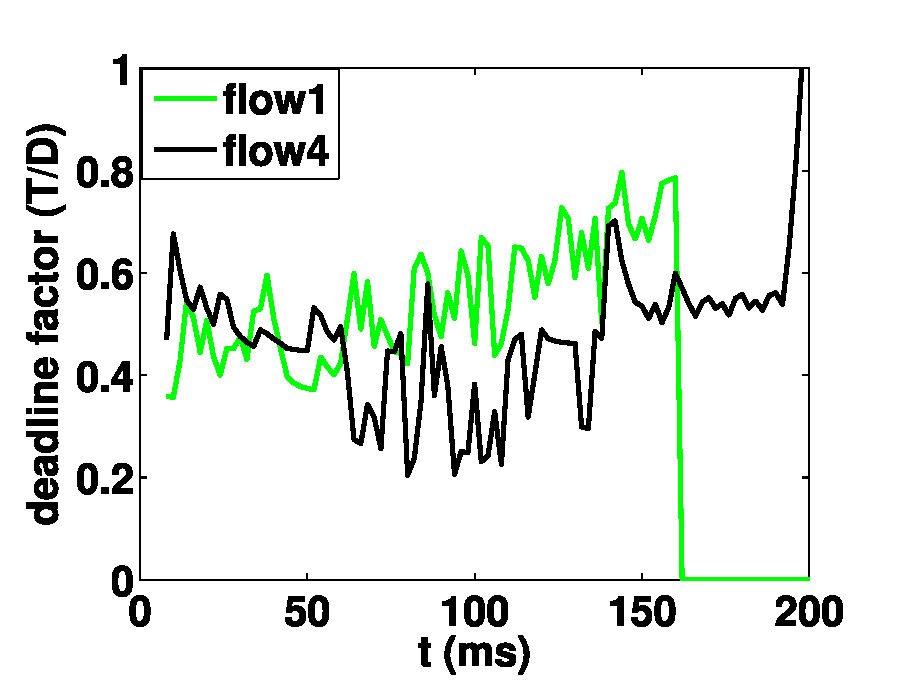
\includegraphics[width=0.5\columnwidth]{figures/LPD/evaluation_1/LPD_factor2.eps}}%
  %\hspace{7em}%
  \subcaptionbox{flow$_1$和flow$_4$的拥塞程度\label{LPD_Evaluation_Motivation:subfig4}}
      {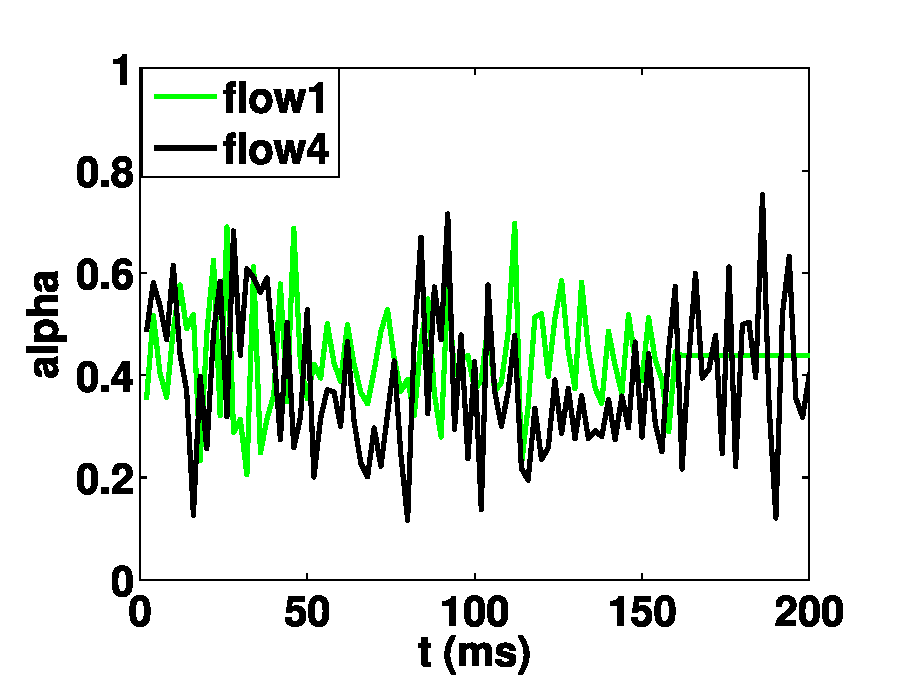
\includegraphics[width=0.5\columnwidth]{figures/LPD/evaluation_1/LPD_alpha2.eps}}
  \caption{LPD下4条流的性能,使用和 D$^{2}$TCP相同的参数}
  \label{evalution_cases_principle_fig}
\end{figure}


\begin{figure}[h]
  \centering%
  \subcaptionbox{流的带宽\label{LPD_Motivation:subfig3}} %标题的长度,超过则会换行,如下一个小图。
    {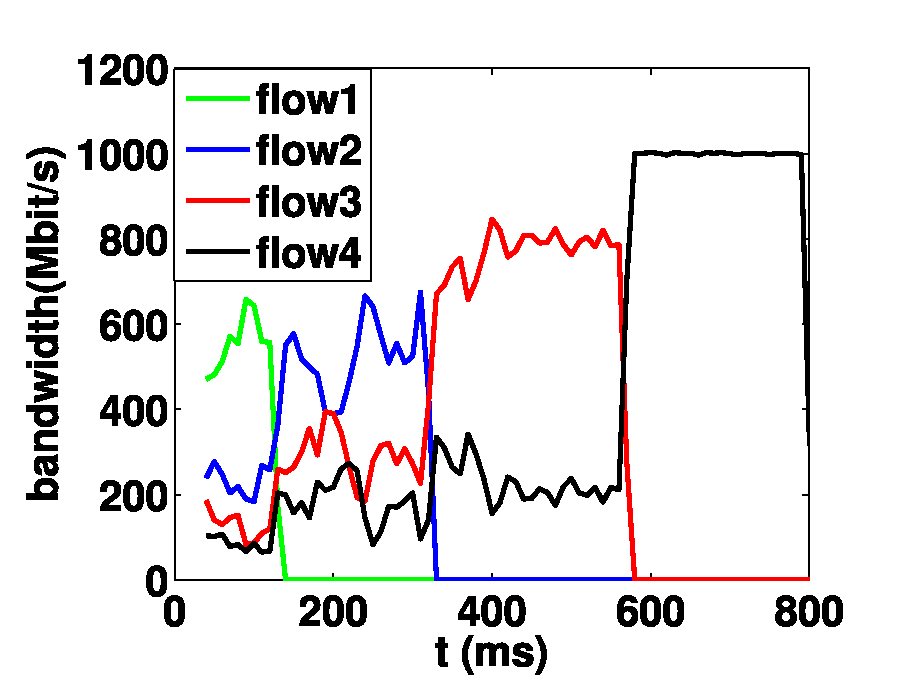
\includegraphics[width=0.5\columnwidth]{figures/LPD/evaluation_1/LPD_bandwidth.eps}}%
  \subcaptionbox{拥塞窗口\label{LPD_Motivation:subfig4}}
      {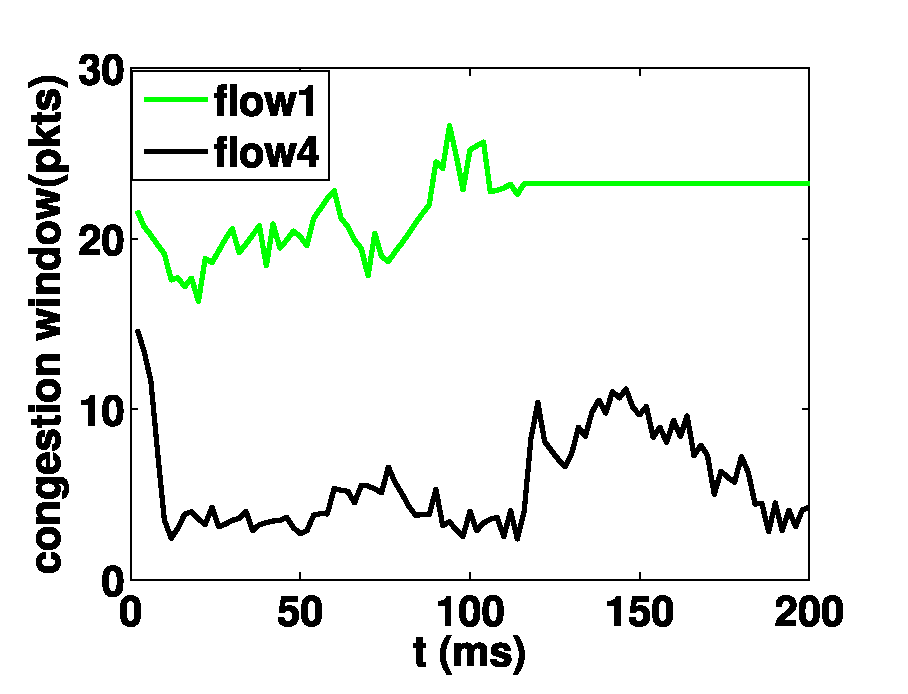
\includegraphics[width=0.5\columnwidth]{figures/LPD/evaluation_1/LPD_window.eps}}
  \subcaptionbox{交换机队列长度\label{LPD_Motivation:subfig5}}%标题的长度,超过则会换行,如下一个小图。
    {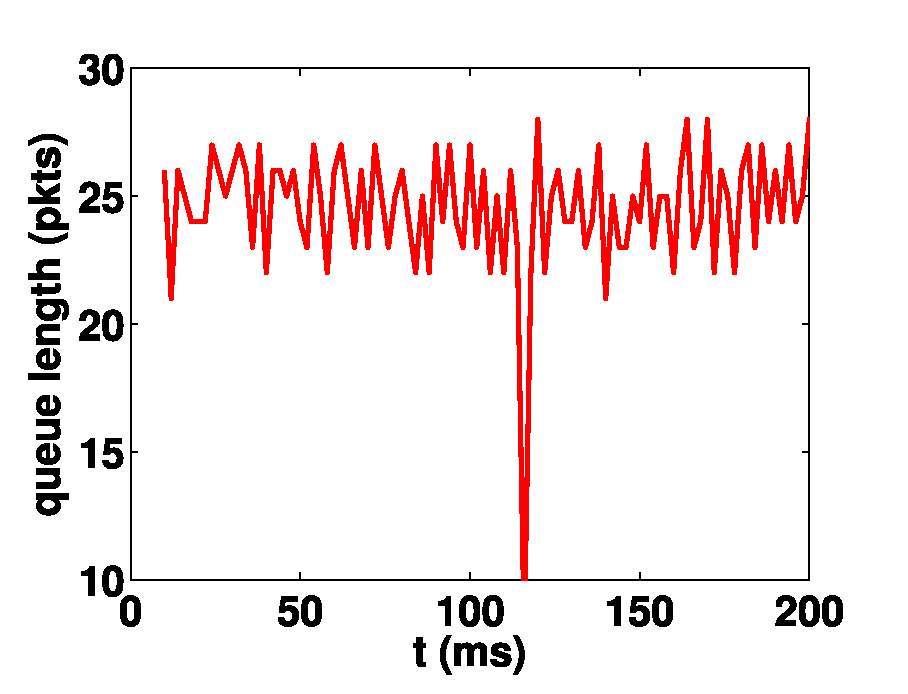
\includegraphics[width=0.5\columnwidth]{figures/LPD/evaluation_1/LPD_queue.eps}}%
  %\hspace{7em}%
  \subcaptionbox{flow$_1$和flow$_4$的拥塞因子\label{LPD_Motivation:subfig6}}
      {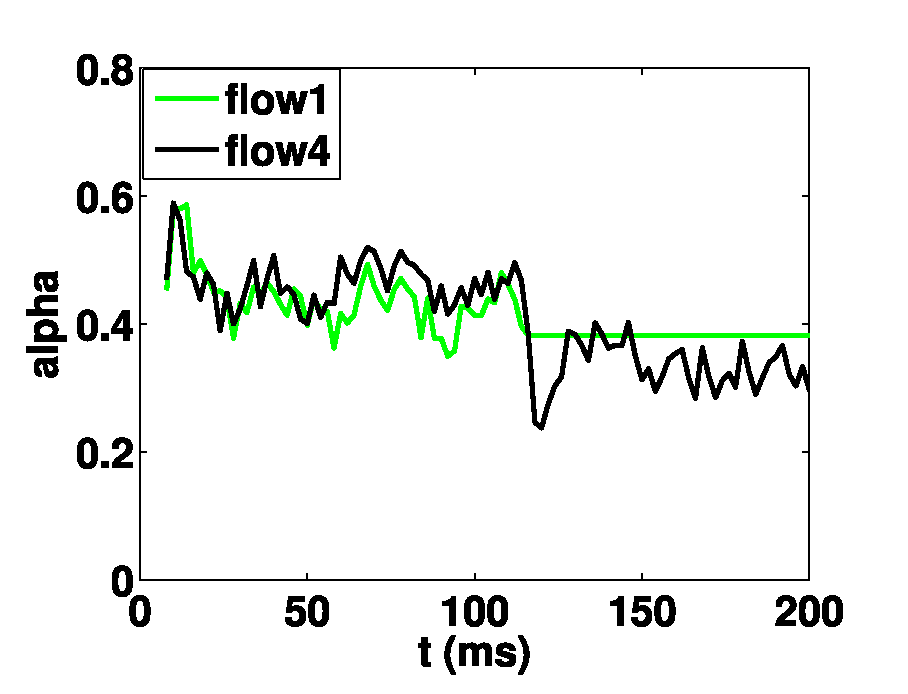
\includegraphics[width=0.5\columnwidth]{figures/LPD/evaluation_1/LPD_alpha.eps}}
  \caption{LPD-t下4条流的性能,使用和 D$^{2}$TCP相同的参数}
  \label{evalution_cases_fig}
\end{figure}



本文首先将LPD应用到\ref{sec_LPD:Motivation}节研究动机介绍的实例中。
虽然此例不是一个典型的OLDI场景,
但是可以用它来检查LPD是否能够帮助更多的流量达到最终期限,
特别是在负载较重的情况下测试LPD的性能。
使用与D$^2$TCP相同的期限因子d=T/D,改动LPD,称之为LPD-d。
在相同的设置下,如图\ref{evalution_cases_principle_fig}(a)所示,只有flow$_2$在LPD-d下错失期限(deadline),
为了更好地理解LPD优于D$^2$TCP和DCTCP的原因,
我们在图\ref{evalution_cases_principle_fig}中给出了LPD下流状态的更多细节。


图\ref{evalution_cases_principle_fig}显示每条流的带宽,以及拥塞窗口w,
期限因子d和flow$_1$与flow$_4$的网络拥塞程度$\alpha$的情形。
与图\ref{LPD_Motivation}对比可以看出,随着流发送,
flow$_1$和flow$_4$之间拥塞窗口之间的差异变得更大,而flow$_1$和flow$_4$的期限因子和网络负载变化不大。
这是因为选择正比负载差分策略,当网络拥塞程度增加时,flow$_1$和flow$_4$有更大的带宽分配差异。
如图\ref{evalution_cases_principle_fig}(a)所示,最终,LPD-d比D$^2$TCP错过期限的流的数目更少。



为了进行比较,设置$t_{max}$ = 800ms,并且在相同的实验环境中测试LPD-t。
如图\ref{evalution_cases_fig}(a)所示,使用LPD-t,所有流在截止期限之前完成传输,
这是因为使用LPD-t,截止时间更近的流会获得更多的带宽,
例如有带宽大小关系:flow$_1>$flow$_2>$flow$_3>$flow$_4$。
图\ref{evalution_cases_fig}描述了LPD-t内部状态,
与LPD-d和D$^2$TCP相比,
如图\ref{evalution_cases_fig}(c)与图\ref{evalution_cases_fig}(d)所示,尽管流计算出的网络负载(即每条流计算的$\alpha$值)基本相同,
但如图\ref{evalution_cases_fig}(d)所示,不同截止期限的数据流的拥塞窗口差异很大。
例如,在前200 ms时间内,flow$_1$获得约$55\%$的带宽,而flow$_4$仅获得$10\%$的带宽。
图\ref{evalution_cases_fig}(c)显示在开始200ms时间内交换机的队列长度,
可以看到,交换机的队列在阈值$K = 25$附近表现出小的波动。
队列在128$ms$处突然下降是由于flow$_1$在此时间点完成传输,
此后,队列很快被未传输完成的数据包填充,
由此还可以看到LPD数据流可以很快的填充交换机队列,从而充分利用链路带宽。
\begin{figure}[H] 
  \centering
  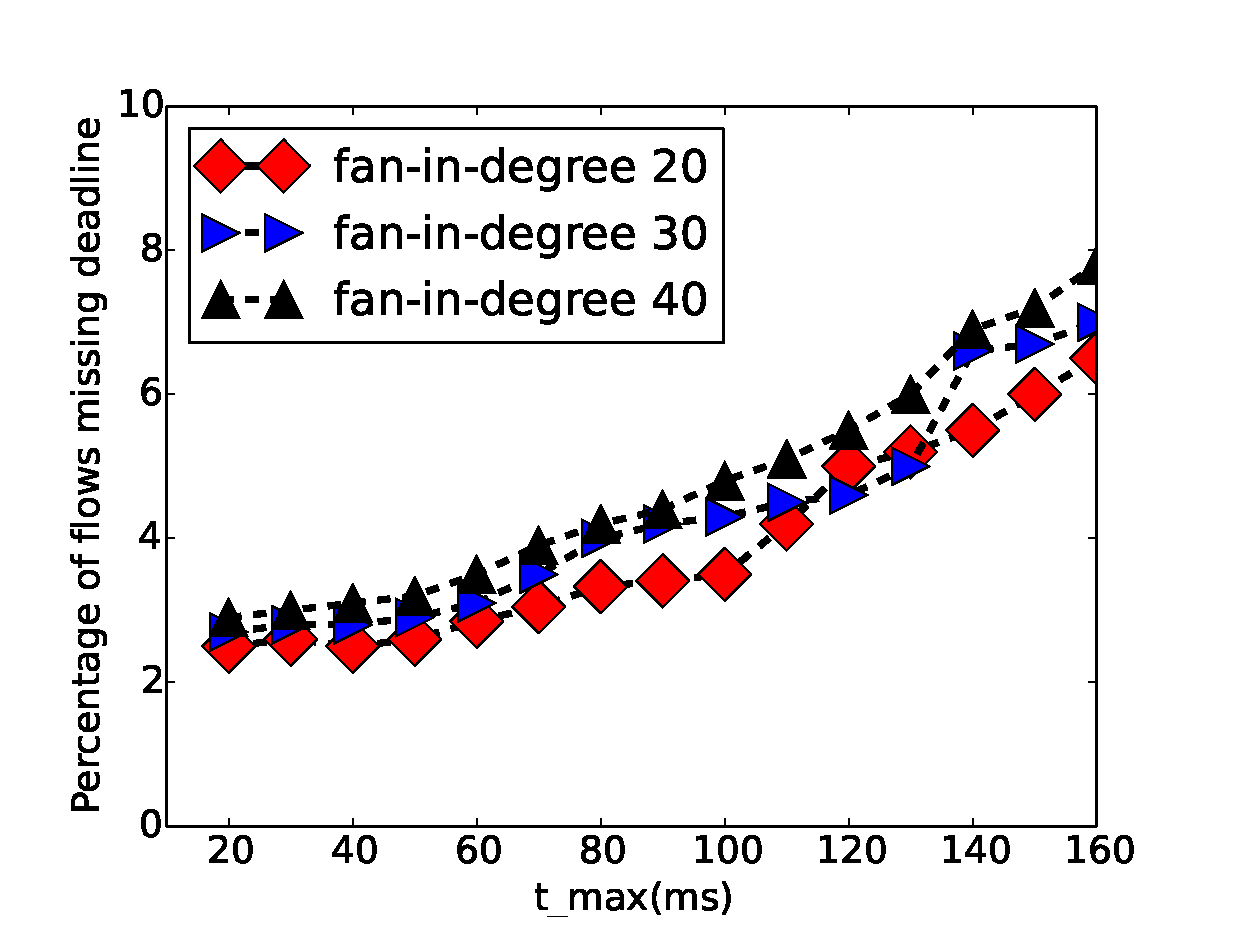
\includegraphics[width=0.8\columnwidth]{figures/LPD/evaluation_3/DMAX.eps}
  \caption{变化 $t_{max}$的影响}
  \label{tmax-fig}
\end{figure}

\subsection{参数选择}
LPD-t和LPD-e必须设置适当的上限$t_{max}$和$s_{max}$。
此处本文只讨论$t_{max}$,因为$s_{max}$有类似的作用。
从LPD-t的等式(\ref{LPD-t-eq})可以看出如果$t_{max}$变大,惩罚函数f就变小。
从(\ref{tmax}),得知对于C = 1Gbps,K = 25,RTT = 1ms,最大数据包大小为1500B,
当并发数据流数量为20,30,40时,对应的$t_{max}$应小于$6 * t_1$,$4 * t_1$,$3 * t_1$。
如果$t_{max}$太大,区分不同期限的流的能力也变弱。
使用OLDI应用来检查$t_{max}$对LPD-t的性能影响,
其中流的截止期限都设置在20ms内,
变换$t_{max}$从20ms变化到160ms(即$t_1 <t_{max} <8 * t_1$)。
图\ref{tmax-fig}描述了不同$t_{max}$下错失期限的流数目,
而扇入度(fan-in-degree,即同时到达根节点的流的数目)分别是20,30和40。


从图\ref{tmax-fig}可以看出,
当$t_{max} $<80ms时,即$t_{max}$不超过最大截止期限的4倍时,使用LPD-t,少于$5\%$的流错过截止期限。
LPD-t的性能总是比D$^2$TCP优异(D$^2$TCP在扇入度分别是20,30和40时错过期限的比例分别为$3.45\%$,$4.96\%$和$5.45\%$)。
而且在这个范围内,使用不同$t_{max}$,LPD的性能差异较大。
然而,当$t_{max}$很大时,例如,当$t_{max}>$120ms(即6倍于截止期限)时,
LPD-t的性能受到极大的损害,并且比D$^2$TCP差。


\subsection{仿真测试}

\subsubsection{简单拓扑测试}
\begin{figure}[H] 
  \centering
  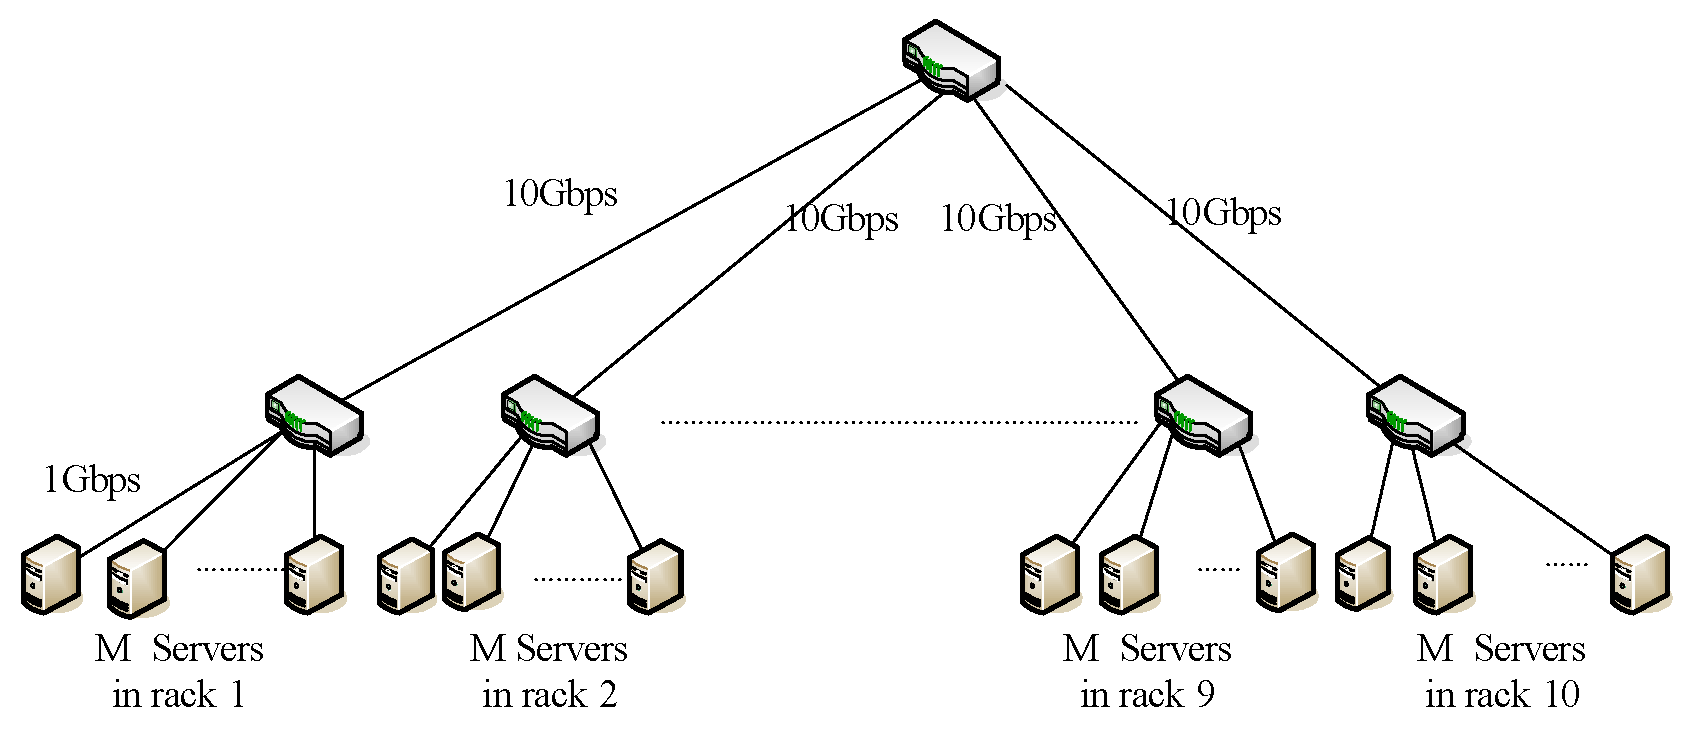
\includegraphics[width=0.9\columnwidth]{figures/LPD/DataCenter.eps}
  \caption{简单的数据中心拓扑}
\label{DataCenterTop-fig}
\end{figure}

为了测试在数据中心下LPD-e的性能,如图\ref{DataCenterTop-fig}所示,我们构建了一个三级树形拓扑。
在这个拓扑中,我们构建10个机架,每个机架由M = 40个服务器组成,机架连接到顶层的TOR交换机。
服务器和交换机之间的链路带宽为1Gbps。
所有TOR交换机通过10Gbps链路连接到根交换机。
在ns-2中构建这种三级树形拓扑,在这个中等数据中心拓扑下,我们评估LPD-e的性能。

和之前工作\cite{DCTCP,D2TCP,L2DCT}类似,设置交换机的标记阈值K=20,并将传播延迟d设置为100us。 
TCP重新传输超时(RTO)设置为10ms,每个发送端初始拥塞窗口设置为12。
考虑在数据中心内,很多大小是200 KB以内的数据流是有期限的,因此设置$s_{max}$ = 200KB。
假设流的大小遵循Pareto分布,Pareto参数为1.2,流的平均大小为50KB。
将流截止期限设置为20,30和40 ms。
对于LPD,将$t_{max}$设置为80 ms。
假设OLDI应用的扇入度从20到40不等,OLDI的扇入度代表了不同程度的网络拥塞。
此外,在所有模拟的服务器中,使用10台服务器产生背景流量。
由于查询结果被返送给OLDI应用程序的根节点,而且所有有期限的流的启动时间基本相同。
所以,如果使用传统的TCP,因为大量并发的小流量共享一个瓶颈链路往往会导致严重的拥塞,因此可能会导致Incast问题\cite{Incast08}。

\begin{figure}[h]
\centering
\subcaptionbox{紧急期限(20ms)}
 {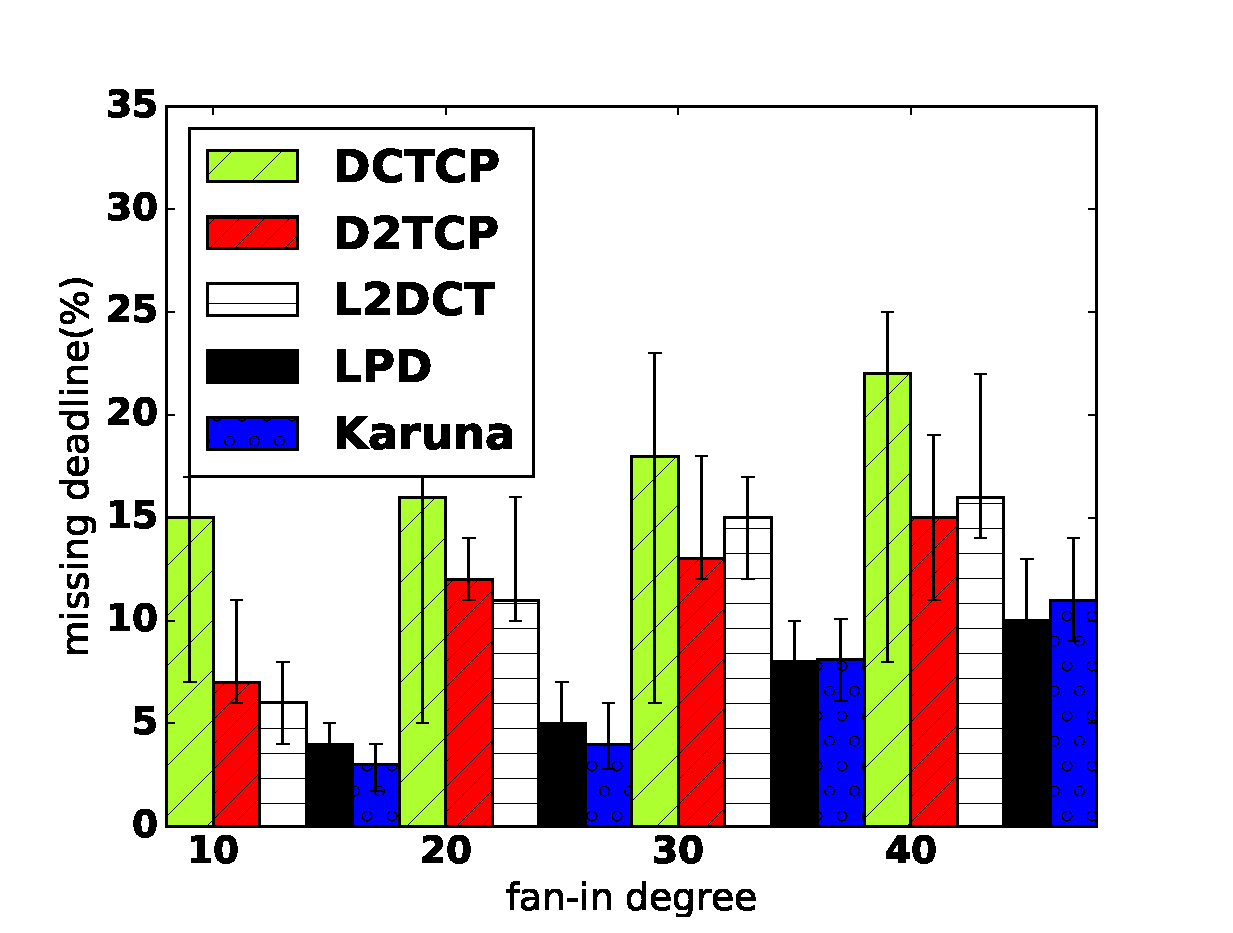
\includegraphics[width=0.32\columnwidth]{figures/LPD/old/tight.eps}}
\subcaptionbox{中等期限(30ms)}
{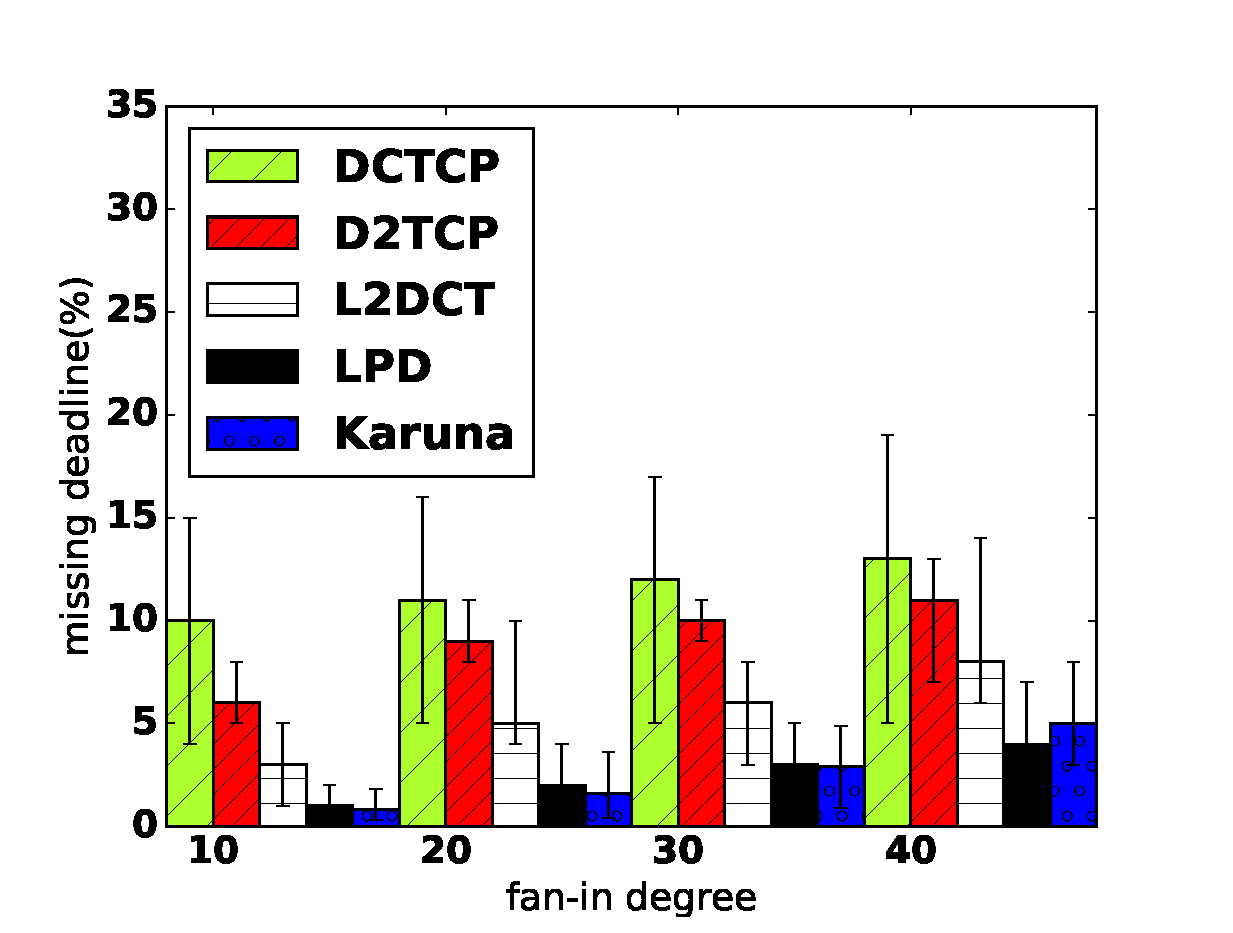
\includegraphics[width=0.32\columnwidth]{figures/LPD/old/moderate.eps}}
\subcaptionbox{松弛期限(40ms)}
{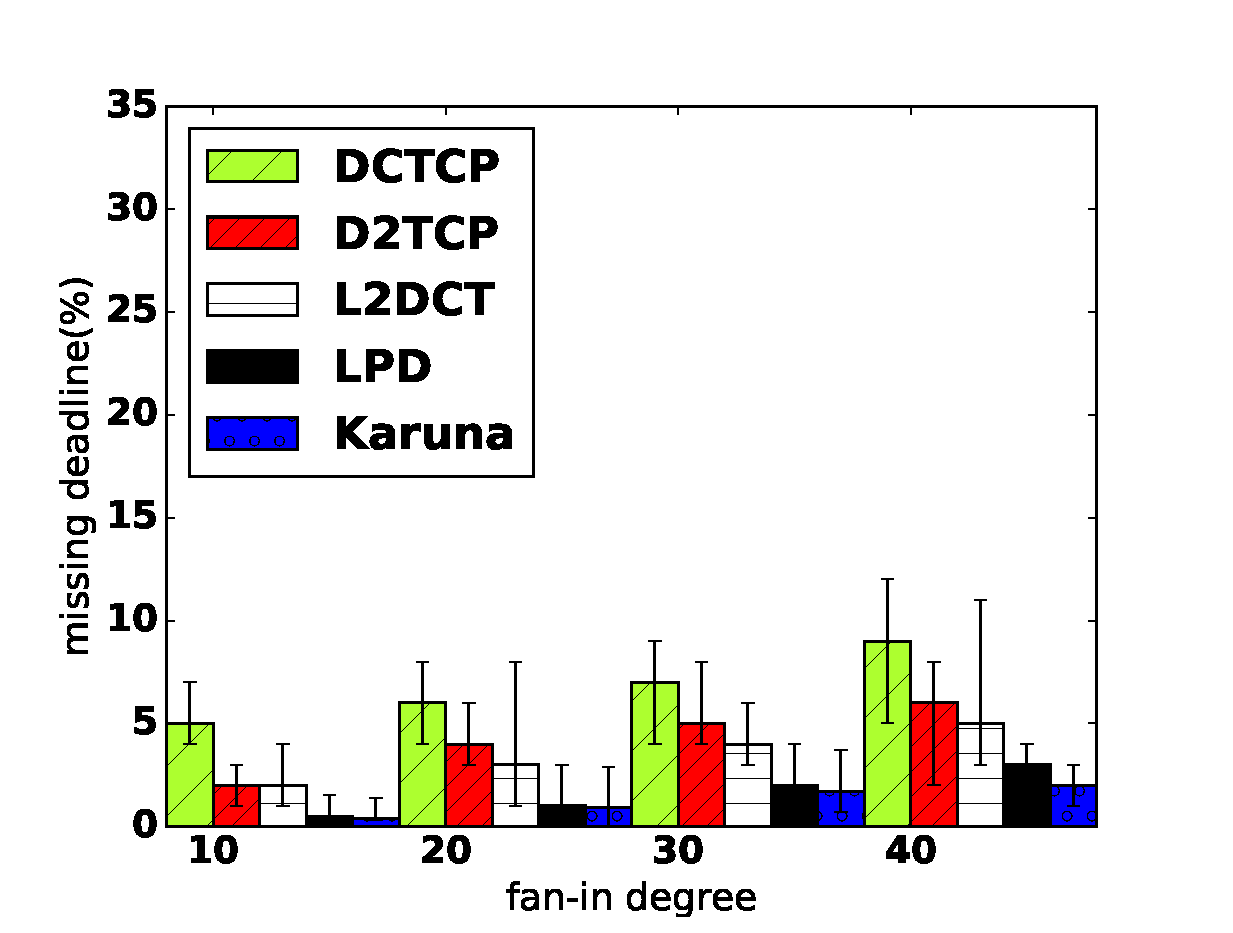
\includegraphics[width=0.32\columnwidth]{figures/LPD/old/lax.eps}}
\caption{DCTCP, D$^2$TCP, L$^2$DCT ,Karuna 和 LPD-e下OLDI应用错失期限的比例对比}
\label{Incast-dc-top-fig}
\end{figure}


\begin{figure}[h]
\centering
\subcaptionbox{紧急期限(20ms)}
 {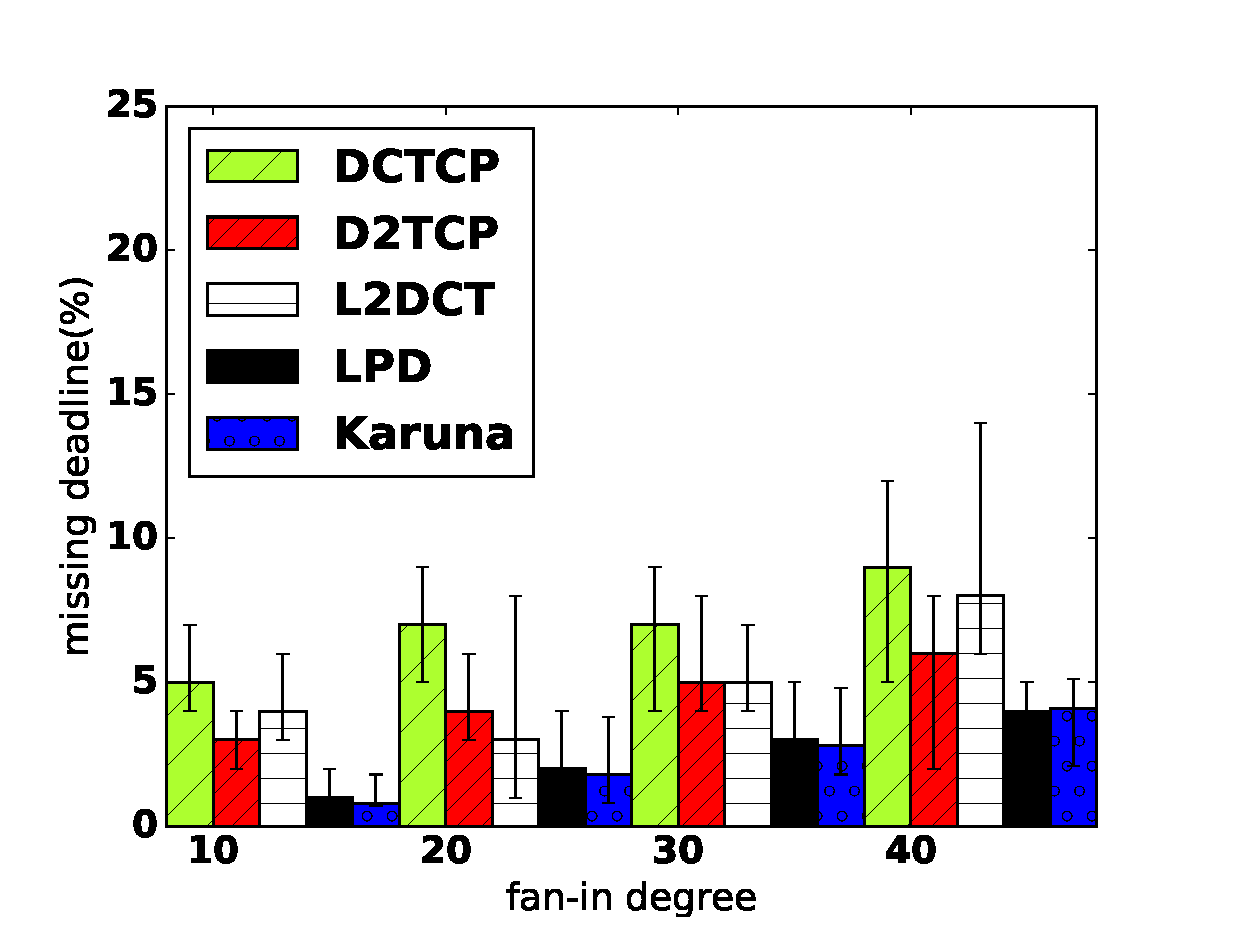
\includegraphics[width=0.32\columnwidth]{figures/LPD/old/tight1.eps}}
\subcaptionbox{中等期限(30ms)}
{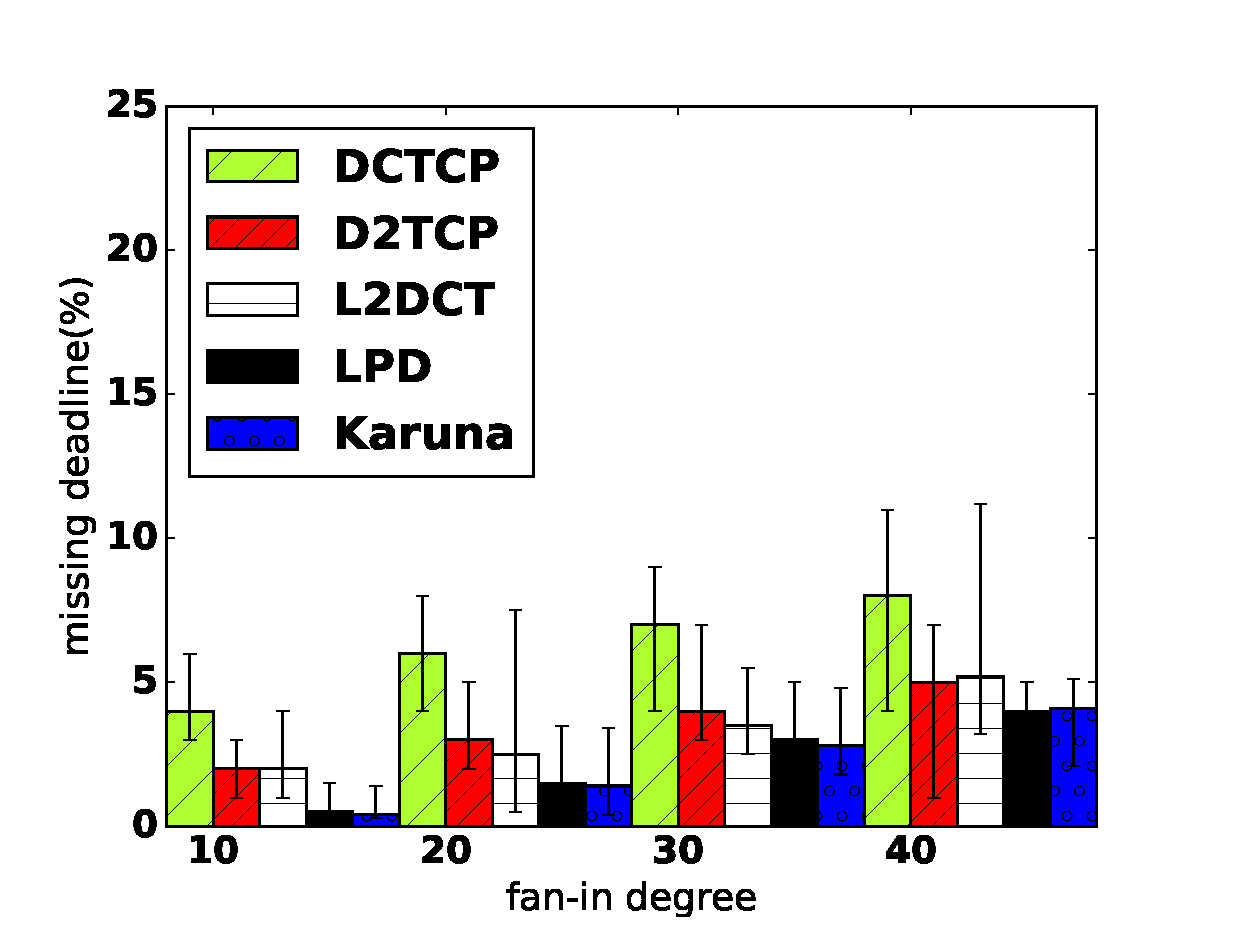
\includegraphics[width=0.32\columnwidth]{figures/LPD/old/moderate1.eps}}
\subcaptionbox{松弛期限(40ms)}
{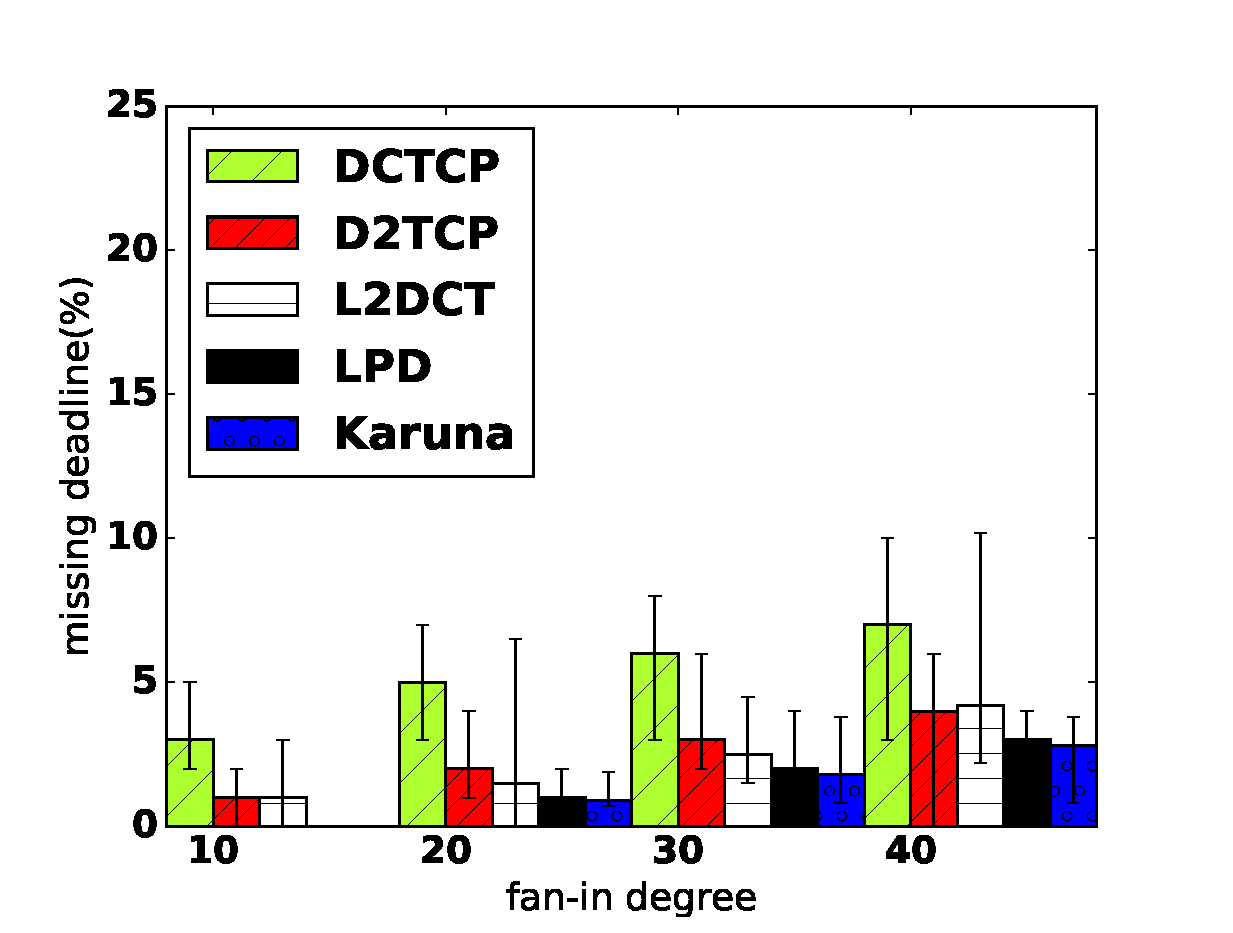
\includegraphics[width=0.32\columnwidth]{figures/LPD/old/lax1.eps}}
\caption{DCTCP, D$^2$TCP, L$^2$DCT ,Karuna 和 LPD-e,流大小分布为Pareto分布的错失期限比例}
\label{miss-dc-posson-fig}
\end{figure}

\begin{figure}[h]
\centering
\subcaptionbox{紧急期限(20ms)}
 {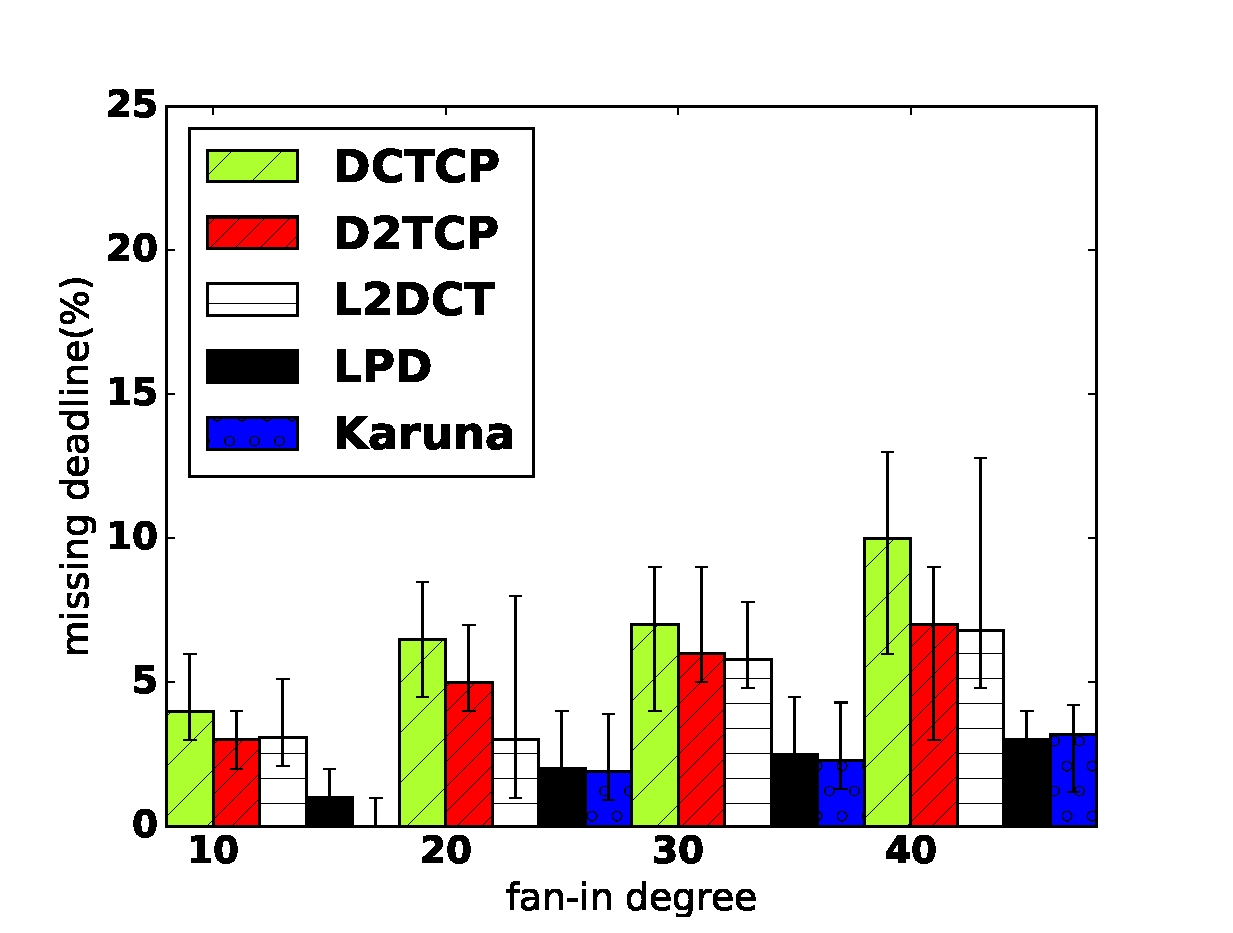
\includegraphics[width=0.32\columnwidth]{figures/LPD/old/tight2.eps}}
\subcaptionbox{中等期限(30ms)}
{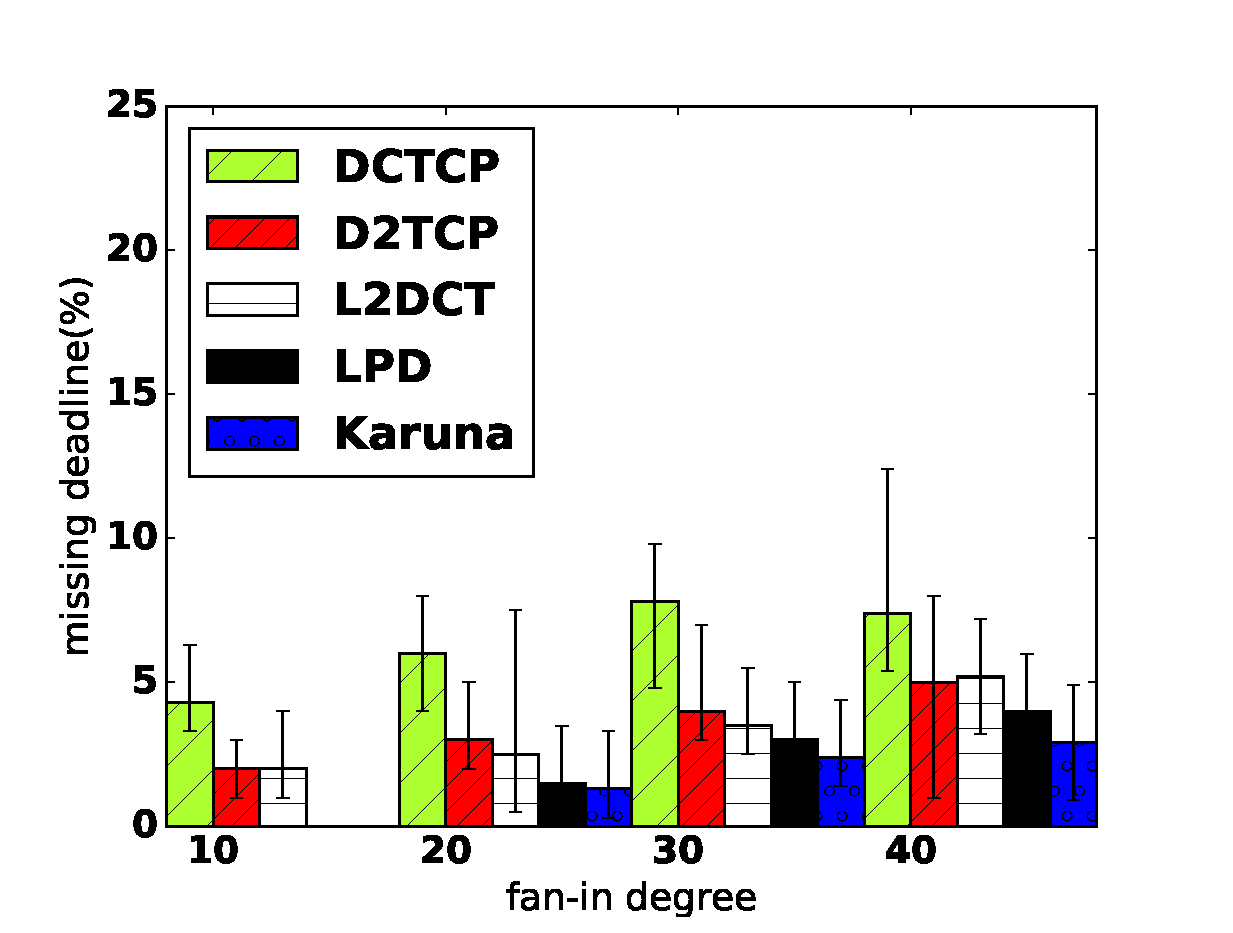
\includegraphics[width=0.32\columnwidth]{figures/LPD/old/moderate2.eps}}
\subcaptionbox{松弛期限(40ms)}
{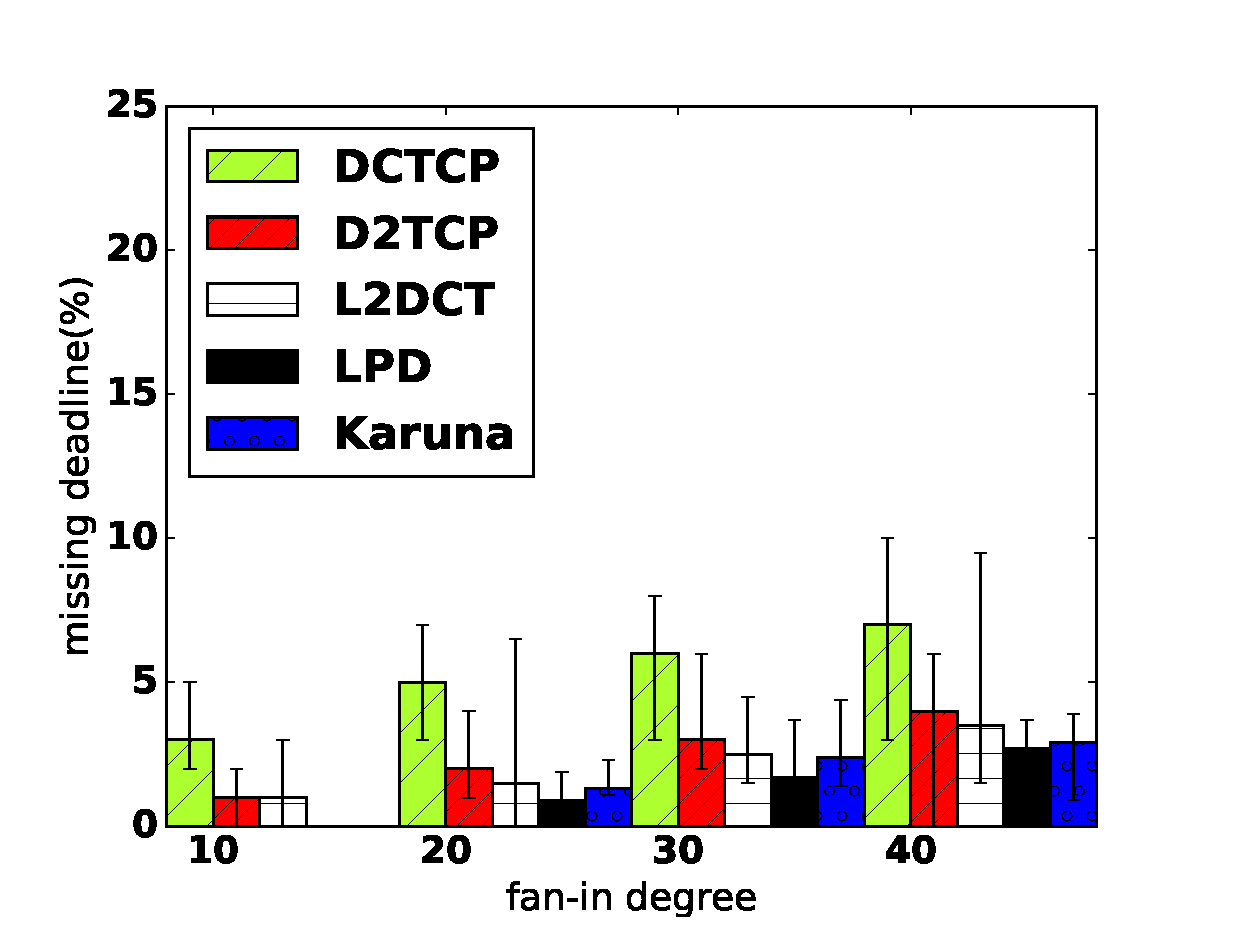
\includegraphics[width=0.32\columnwidth]{figures/LPD/old/lax2.eps}}
\caption{DCTCP, D$^2$TCP, L$^2$DCT ,Karuna 和 LPD-e,流的期限为随机分布}
\label{miss-dc-uniform-fig}
\end{figure}


图\ref{Incast-dc-top-fig}显示了不同扇入度下流错失期限的百分比。
为了更好的展示LPD的性能,本文使用DCTCP,D$^2$TCP,L$^2$DCT,Karuna和LPD-e作为对比方案。
变换每组实验参数100次,图\ref{Incast-dc-top-fig}显示的结果中,每个柱状图显示错失期限流的百分比的平均值,
其中error bar展示了错失期限的流百分比最小值和最大值。
注意到,L$^2$DCT也是一种基于TCP的拥塞速率控制机制。
与D$^2$TCP类似,L$^2$DCT也使用gamma函数进行拥塞窗口的计算,但是和D$^2$TCP不同的是,L$^2$DCT只使用流大小作为拥塞窗口的调整因子。
实验结果表明LPD-e在网络拥塞程度很重的情形下依然可以根据流的期限进行区分,
因此,相比DCTCP,D$^2$TCP,L$^2$DCT,Karuna等,使用LPD-e使得流错失期限的数目最少。
尽管D$^2$TCP(以及L$^2$DCT)在DCTCP上有所改进,
如图\ref{Incast-dc-top-fig}(c)所示,D$^2$TCP仅仅在期限较宽松的情况下性能比DCTCP有明显的优势,
但对期限很紧的情形,如图\ref{Incast-dc-top-fig}(a)和(b)所示,D$^2$TCP并没有明显的优势。
事实上,对此问题,D$^2$TCP\cite{D2TCP}并没有进行详细讨论。
对于最先进的基于截止期限进行速率控制的方法Karuna \cite{chen2016scheduling},性能平均比LPD-e好$5\%$。
然而,对于并发程度很高的情形(如扇入度为40),此时网络处于重度拥塞,Karuna的性能比LPD差。
其原因是随着网络拥塞程度增加,使用LPD,不同期限的流获得带宽差距越来越大,
从而,数据流获得不同带宽,因而,截止期限更近的流能获取更多的带宽,从而更有可能在截止期限之前完成。



在另一种不同的场景下测试LPD-e性能,
在此场景下,服务器之间相互发送短流,变化每台机架上服务器的数目,
设置短流的到达间隔服从泊松过程(每台服务器每秒钟发送1000条数据流),
而所有其他设置(包括流量大小分布和截止期限)与上述OLDI场景中的设置相同。
图\ref{miss-dc-posson-fig}中描绘每个策略流错失期限数目的百分比。
图中柱状图每个柱呈现的结果包括平均期错过期限的流百分比,
以及进行100次随机实验得到错过期限流的数目的最小和最大值,其中我们可以看到LPD在所有情况下,性能比其他的方法要好。
特别是当负载相对较轻的情况时(即每个机架上的10台服务器发送短流,此时网络拥塞程度较轻),
无论截止期限是近还是远,使用LPD-e流错失期限的数目都是0。
与其他协议相比,除了当网络负载很重的时(即每个机架有40个服务器发送短流量时),
在几乎所有情形下,使用LPD-e,错过截止时间的流的数目降低$50\%$以上。
在负载很重时,与其它协议相比,LPD-e仍然可以将错失期限的流的比例降低至少$30\%$。

假设流大小在2 KB到200 KB范围内均匀分布,
流的期限服从平均值为30 ms,40ms和50ms的指数分布。
其它实验参数和上述其它实验相同,
实验结果结果如图\ref{miss-dc-uniform-fig}所示,不管拥塞的程度是轻微,中等还是重度,LPD-e仍然性能最好。
注意到,在所有的仿真结果中,L$^2$DCT通常可以达到与D$^2$TCP相当的结果,猜测这是由于它们都使用了伽马校正功能。
此外,在大多数情况下,Karuna表现比LPD-e更好,但是在网络负载较重的情况下,
有时LPD-e可以比Karuna表现更好,这是因为LPD-e的设计中遵循 “越拥塞,越区分”的原则,
当网络拥塞程度严重时,不同期限的数据流获得的带宽区分很大,因此更多紧急的数据流能在截止期限之前完成。

\subsubsection{复杂拓扑下测试}
\begin{figure}[H] 
  \centering
  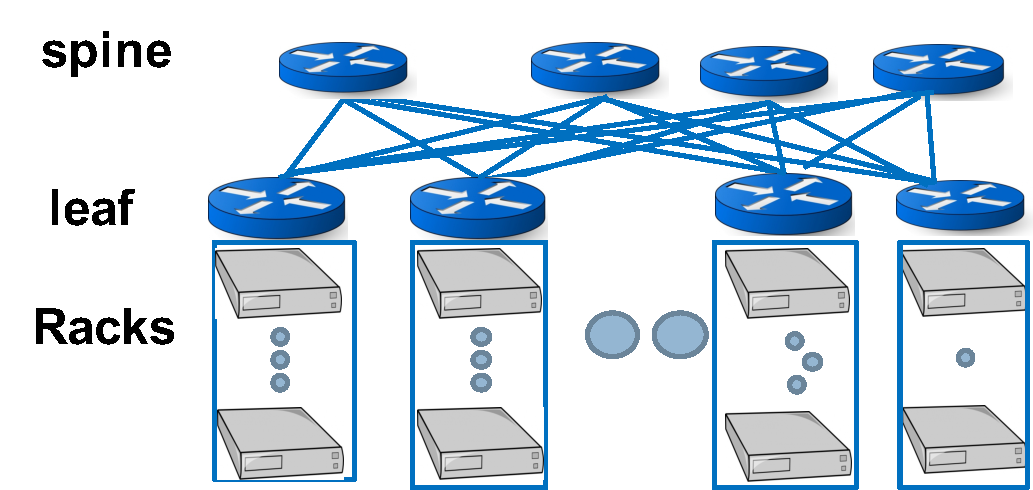
\includegraphics[width=0.8\columnwidth]{figures/LPD/spineleaf.pdf}
  \caption{数据中心spine-leaf拓扑}
\label{DataCenterspineleaf-fig}
\end{figure}

为了展示LPD如何在复杂的数据中心拓扑结构下的性能,
以及LPD在真实流量下的性能,我们在ns-2模拟器中构建了spine-leaf拓扑,拓扑结构如图\ref{DataCenterspineleaf-fig}所示。
在构建的拓扑中,共有144个服务器连接到9个叶子交换机,这9个叶子交换机连接4个主干交换机。
通过主干交换机(4跳)的端到端往返延迟是14.6 us,叶交换机(2跳)的端到端往返延迟是13.3 us。
在这些延迟中,10us的时间是在端节点上,这模拟的是像hadoop这类应用的计算时间。 
TCP重传超时(RTO)设置为10 ms,初始拥塞窗口设置为12。
主干交换机和叶交换机之间的链路容量为$40 Gbps / x$,其中x为超额认购因子,叶节点和终端服务器之间的容量为10Gbps。 
K=64,设置$s_{max}$的默认值是1MB,$t_{max}$=30ms。


\begin{figure}[h]
\centering
\subcaptionbox{紧急期限(20ms)}
 {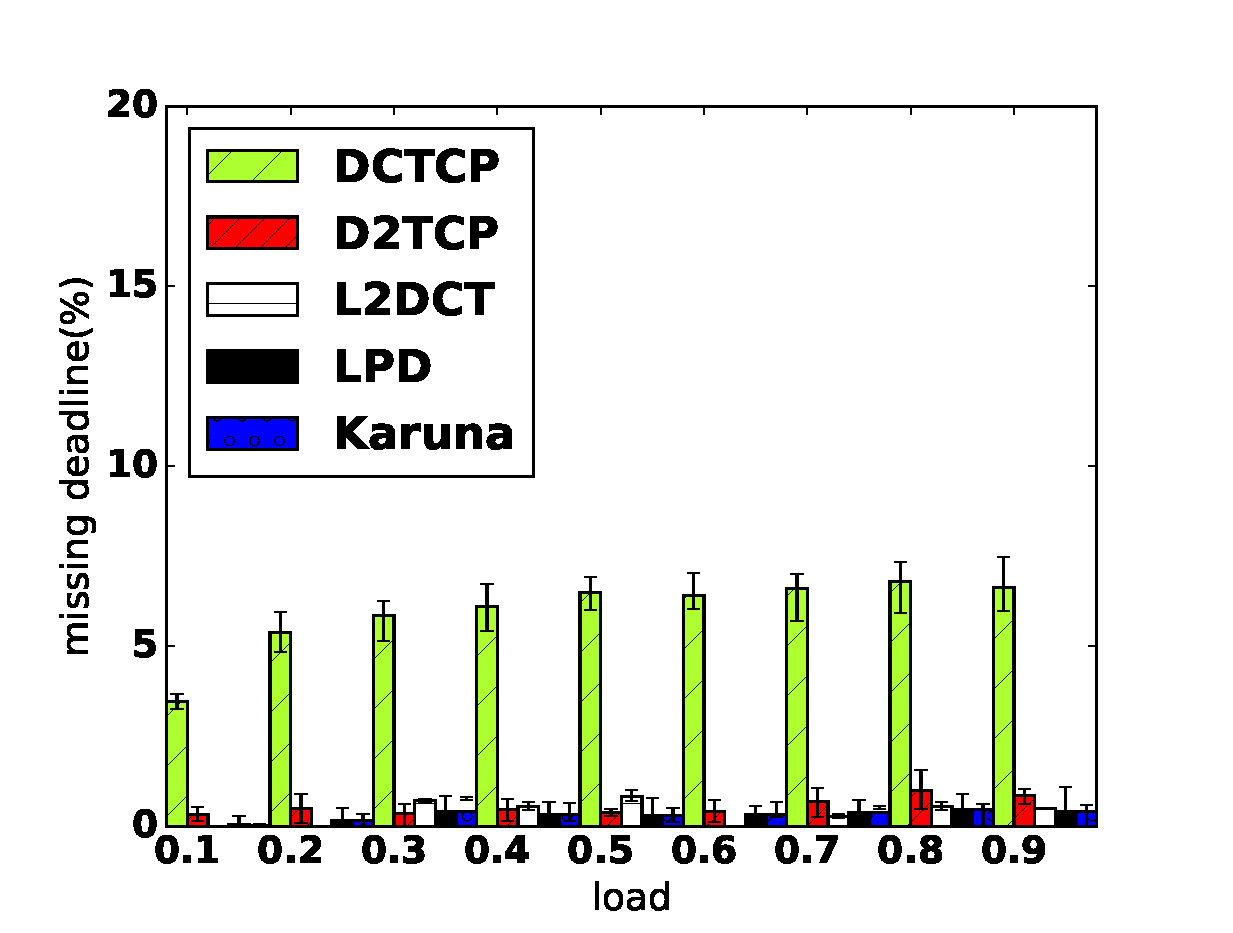
\includegraphics[width=0.32\columnwidth]{figures/LPD/spineleaf/miss_deadline_1.eps}}
\subcaptionbox{中等期限(30ms)}
{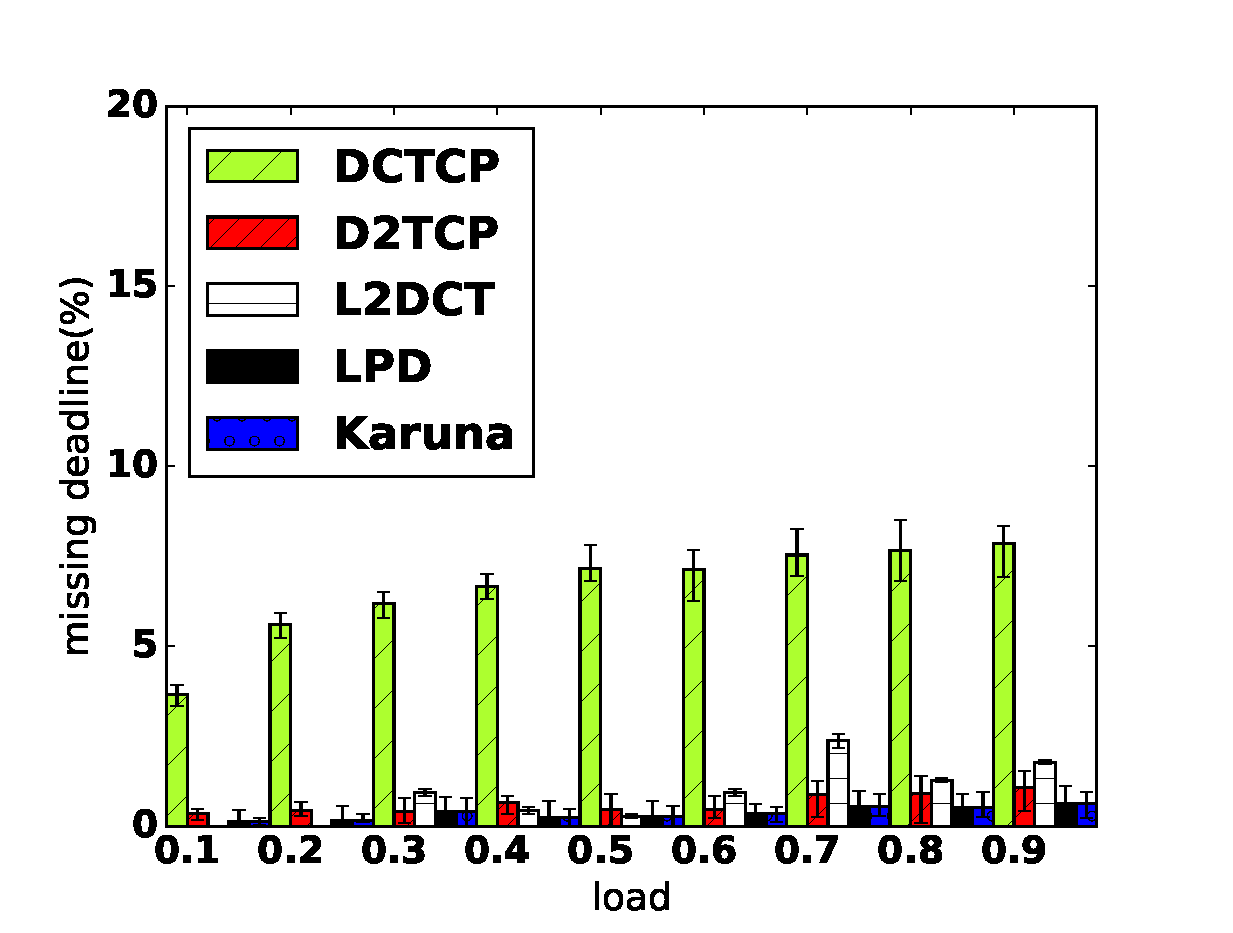
\includegraphics[width=0.32\columnwidth]{figures/LPD/spineleaf/miss_deadline_5.eps}}
\subcaptionbox{松弛期限(40ms)}
{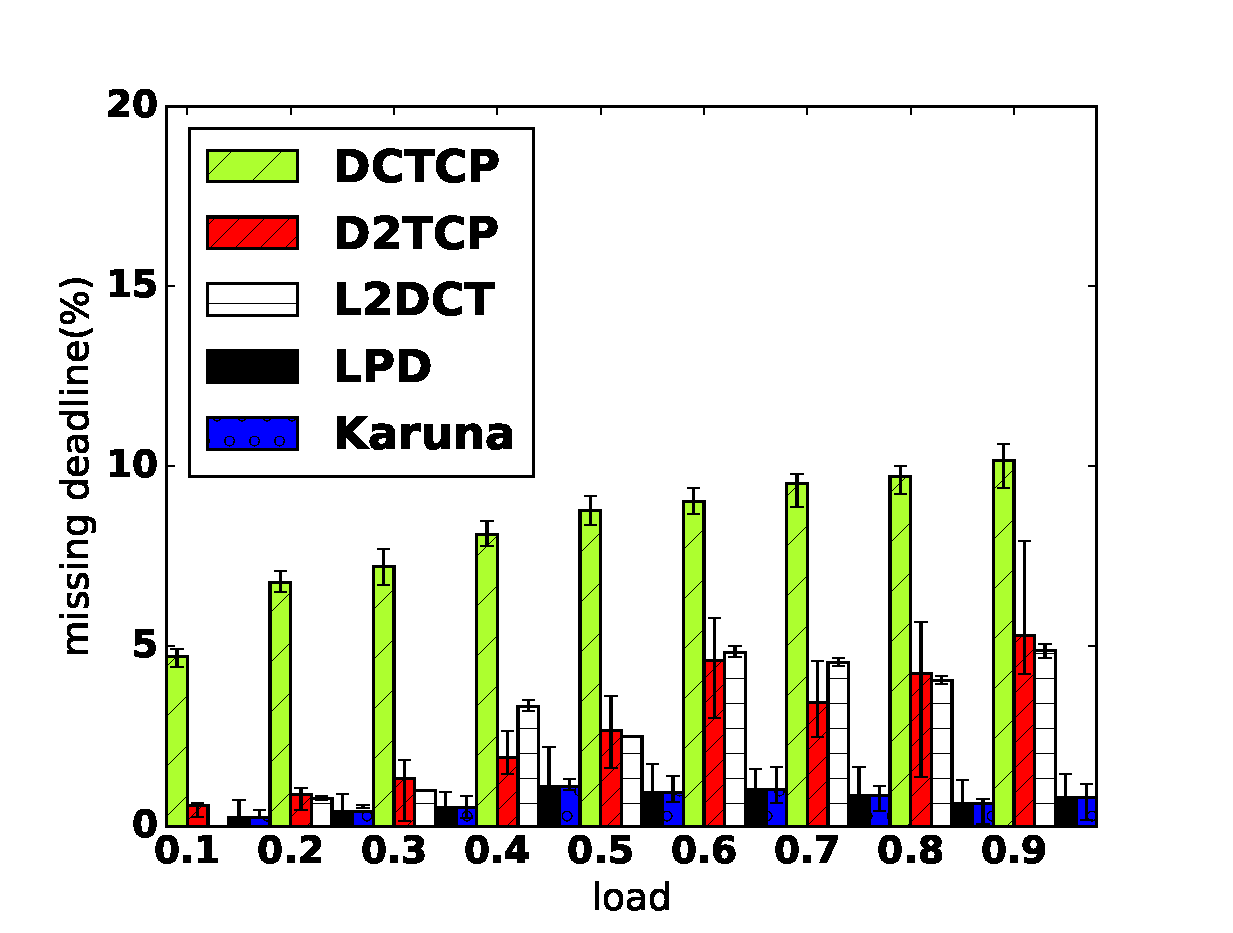
\includegraphics[width=0.32\columnwidth]{figures/LPD/spineleaf/miss_deadline_10.eps}}
\caption{网络搜索应用流量下,LPD-e,D$^2$TCP, L$^2$DCT ,Karuna 和 DCTCP性能对比。流的截止期限是在10ms到30ms的统一分布}
\label{spine-dc-web-10}
\end{figure}



\begin{figure}[h]
\centering
\subcaptionbox{紧急期限(20ms)}
 {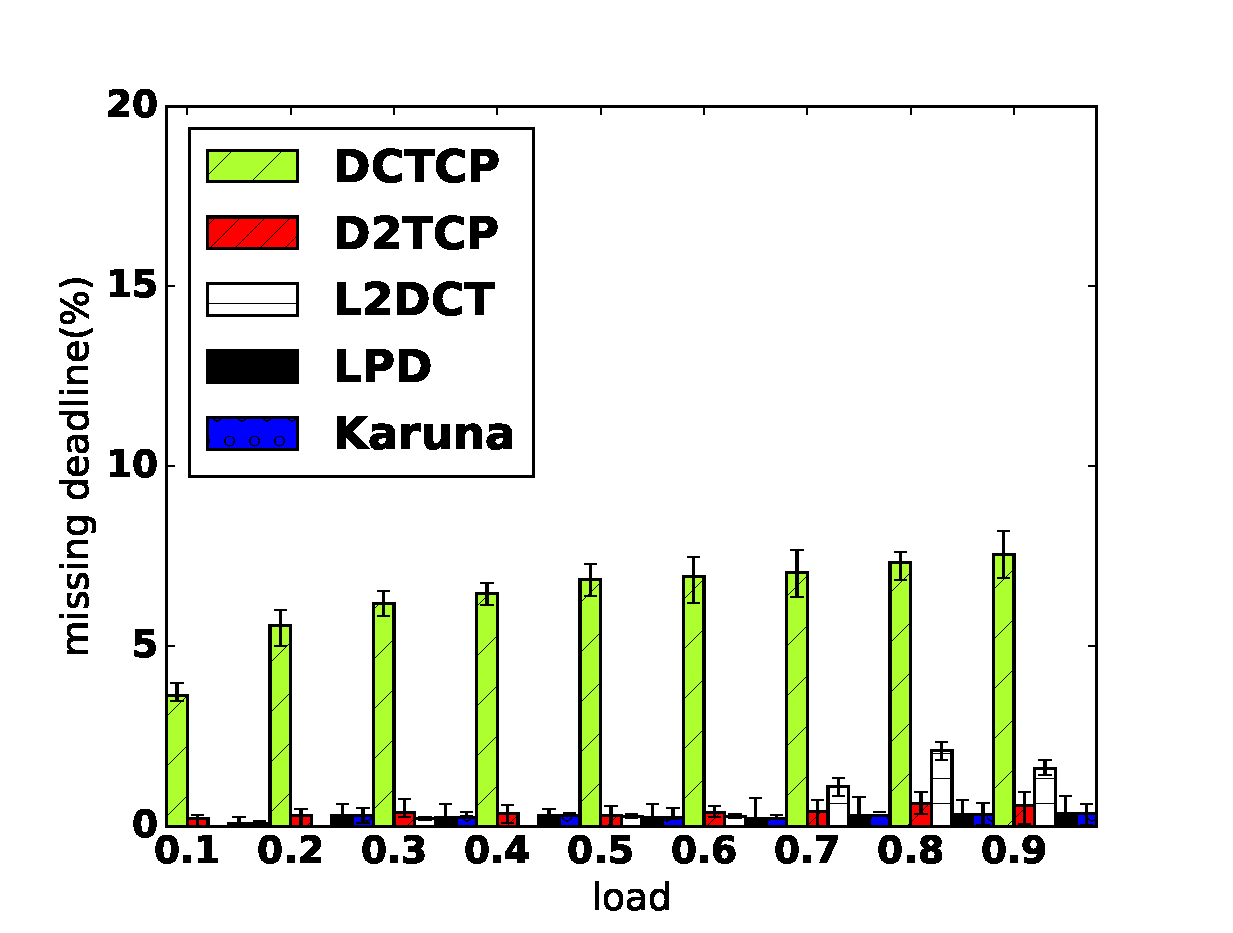
\includegraphics[width=0.32\columnwidth]{figures/LPD/spineleaf/miss_deadline_4.eps}}
\subcaptionbox{中等期限(30ms)}
{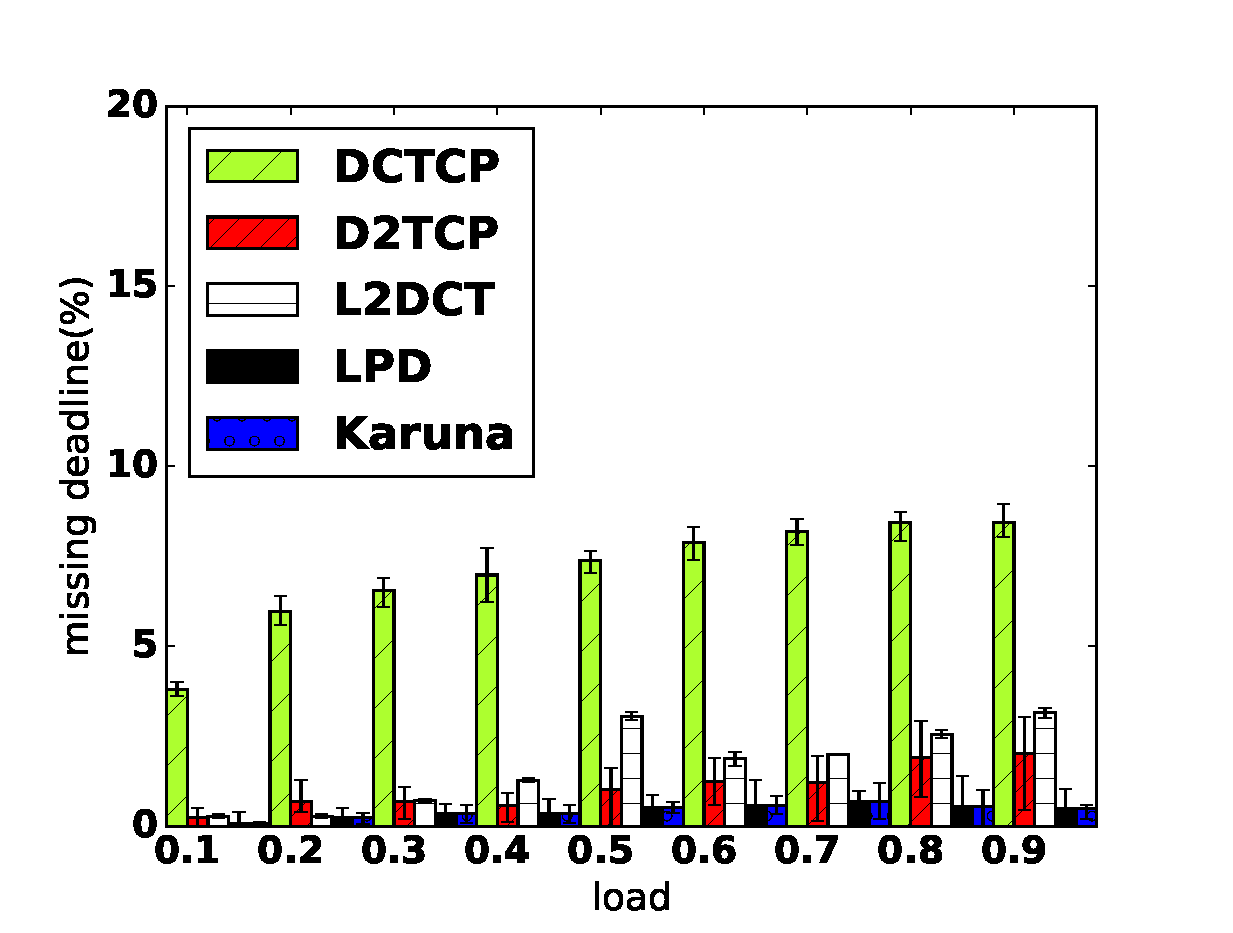
\includegraphics[width=0.32\columnwidth]{figures/LPD/spineleaf/miss_deadline_6.eps}}
\subcaptionbox{松弛期限(40ms)}
{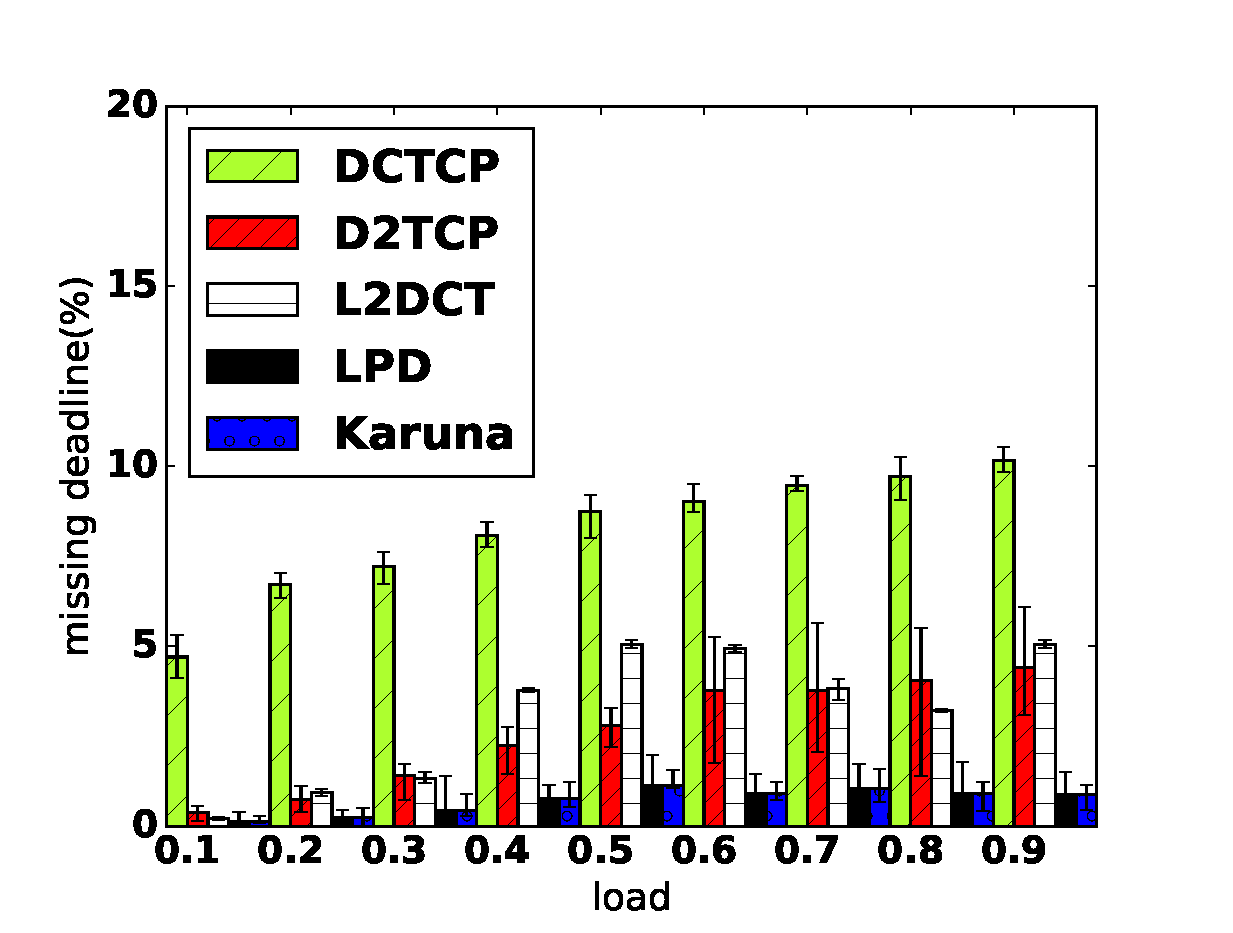
\includegraphics[width=0.32\columnwidth]{figures/LPD/spineleaf/miss_deadline_9.eps}}
\caption{数据挖掘应用流量下,LPD-e,D$^2$TCP, L$^2$DCT ,Karuna 和 DCTCP性能对比。流的截止期限是在10ms到30ms的统一分布}
\label{miss-spine-data-fig}
\end{figure}


本文在实验中使用两个世纪数据中心应用的流量:网络搜索(web search)和数据挖掘(data mining)\cite{DCTCP,pFabric}。
在网络搜索流中,$70\%$的流小于1 MB,超过$50\%$的流在100 KB到1 MB之间。
在数据挖掘流中,超过$80\%$的流是小于10KB的小流,大于1MB的$4\%$的大流占据超过$90\%$的数据量。
在本部分的仿真中,假设数据流的到达服从泊松分布。 
流的源和目标服务器是随机选择的,并且服从均匀分布。
流到达的时间间隔不同,会产生不同程度的网络负载。
当今的数据中心网络往往是超额认购\cite{CloudMirror},
在后续的实验中,本文变更超额认购参数来模拟此。






对于截止期限比较紧的流,本文选择错失期限的流的比例作为评价标准来评价算法。
对于截止期限不敏感的数据流,本文考虑流平均完成时间。
本节测试在延迟敏感的网络负载下LPD的性能。
在实际中,网络搜索等对延迟敏感的业务需要在几毫秒内将计算结果传送给客户端,否则会影响用户体验。
在下面实验中,设置截止期限在10ms到30ms之间均匀的分布。
其余的参数适用默认的值。将超额认购因子x从1改变为10,图\ref{spine-dc-web-10}显示了结果。
需要注意的是,每组实验重复100次,在图中标记处每组的平均值,最大值,最小值。



从图\ref{spine-dc-web-10}可以看出,使用LPD-e有少于1$\%$的数据流错失期限,
而使用DCTCP,D$^2$TCP,L$^2$DCT时,分别有$17\%$,$2.5\%$,$2.4\%$错失期限。
特别是,当负载和超额认购因子很小(load= 0.1,x = 1)时,D$^2$TCP和L$^2$DCT错过期限的流数目是LPD-e的2$\times$。
但是当超额因子和负载较大(load= 0.9,x = 10)时,D$^2$TCP和L$^2$DCT错过期限的流数目是LPD-e的5$\times$。
这是因为随着超额认购因子变大,网络负载变大,
LPD的惩罚函数比D$^2$TCP和L$^2$DCT的gamma校正函数性能更好,因此流错失期限的比例更小。
Karuna,当前最先进的基于期限的拥塞控制方法,有不到$1\%$的流错失期限。
然而,当网络的负载变重(负载= 0.9,x = 10)时,LPD表现比卡Karuna好。
这是因为,当网络负载加重时,使用LPD,不同截止期限的流的拥塞窗口差异更大。
使用数据挖掘应用的结果与之类似,结果如图\ref{miss-spine-data-fig}所示。


\begin{figure}[h]
\centering
\subcaptionbox{流平均完成时间}
 {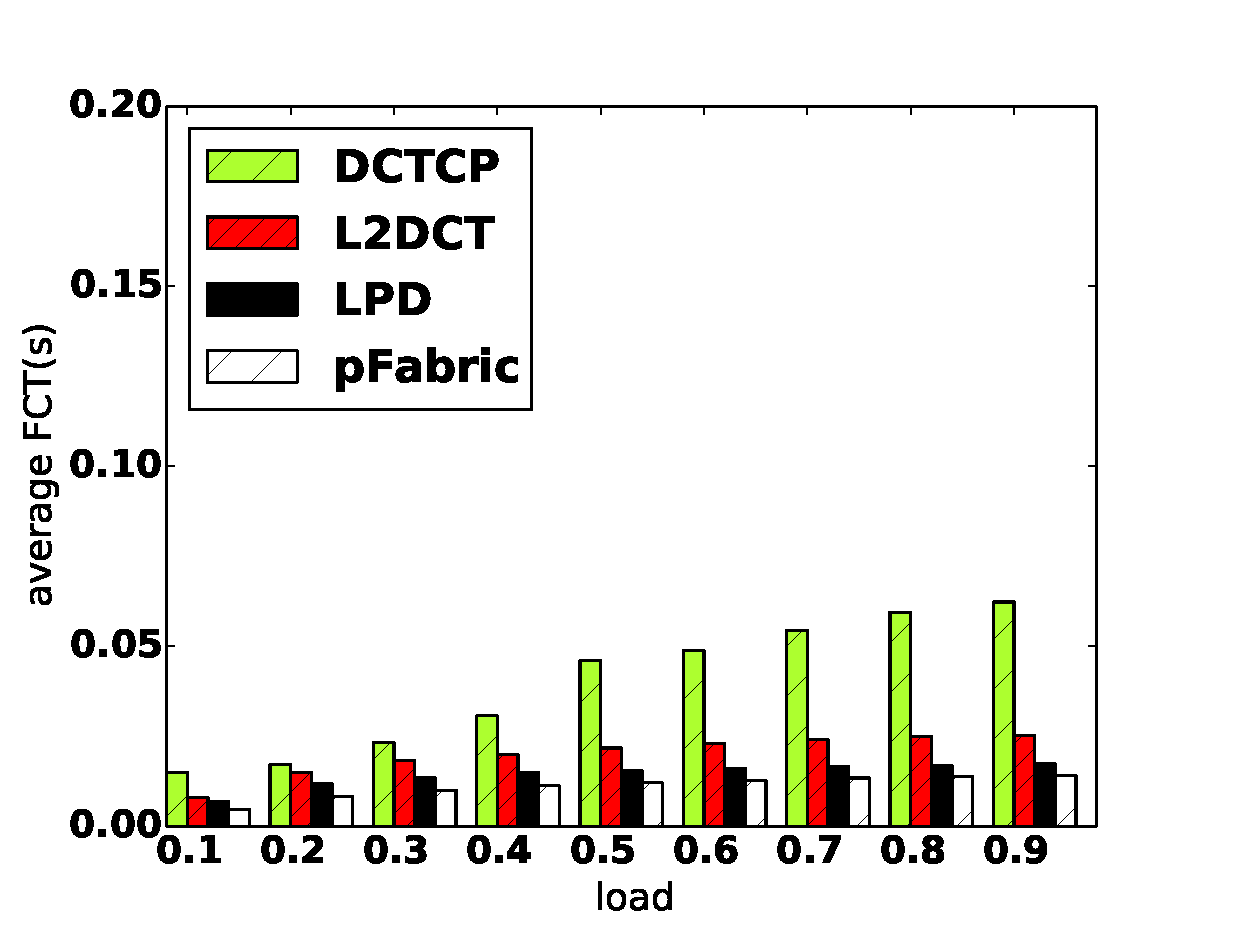
\includegraphics[width=0.32\columnwidth]{figures/LPD/spineleaf/FCT_SEARCH_average.eps}}
\subcaptionbox{(500KB,+$\infty$)}
{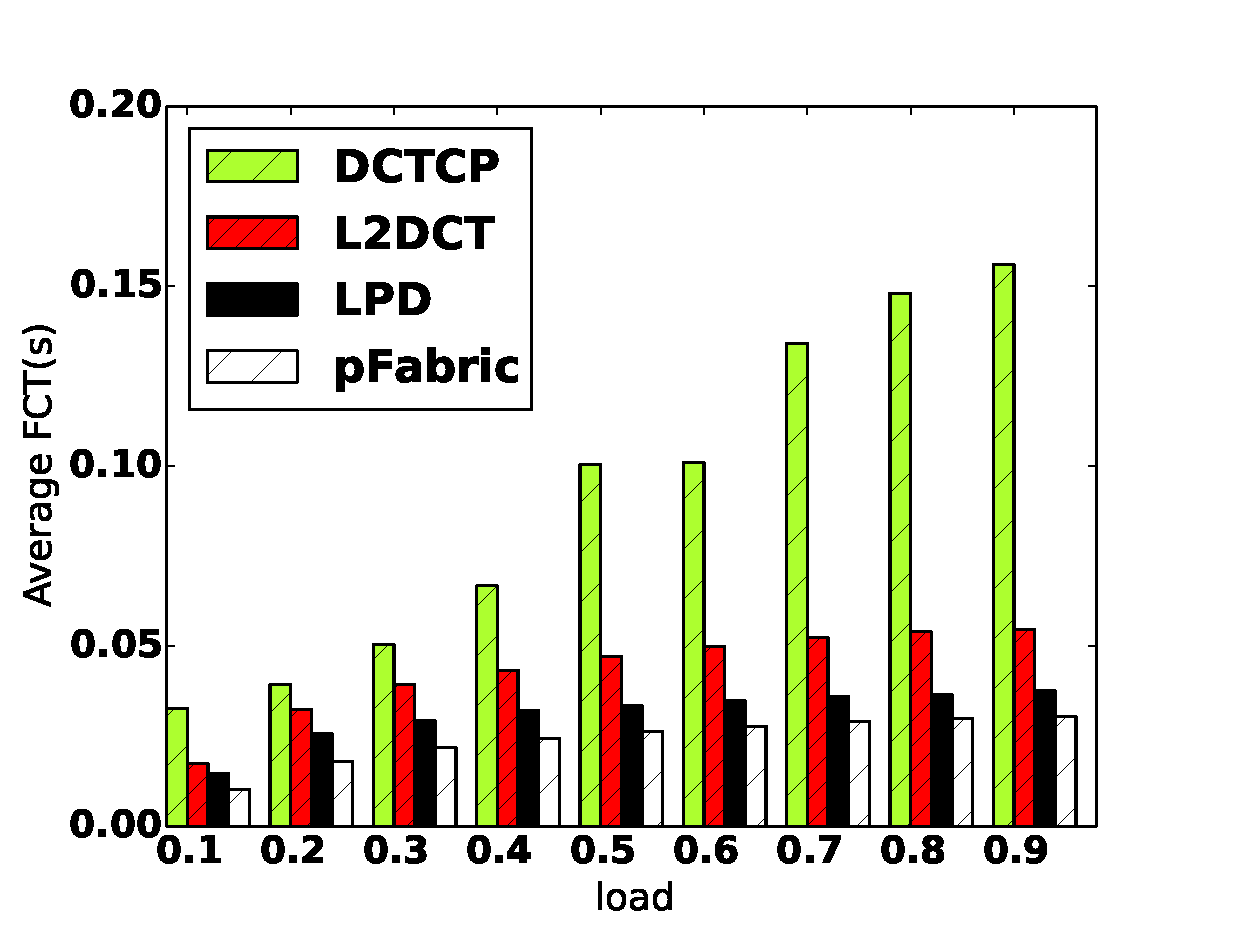
\includegraphics[width=0.32\columnwidth]{figures/LPD/spineleaf/FCT_SEARCH_large.eps}}
\subcaptionbox{(0,100KB)}
{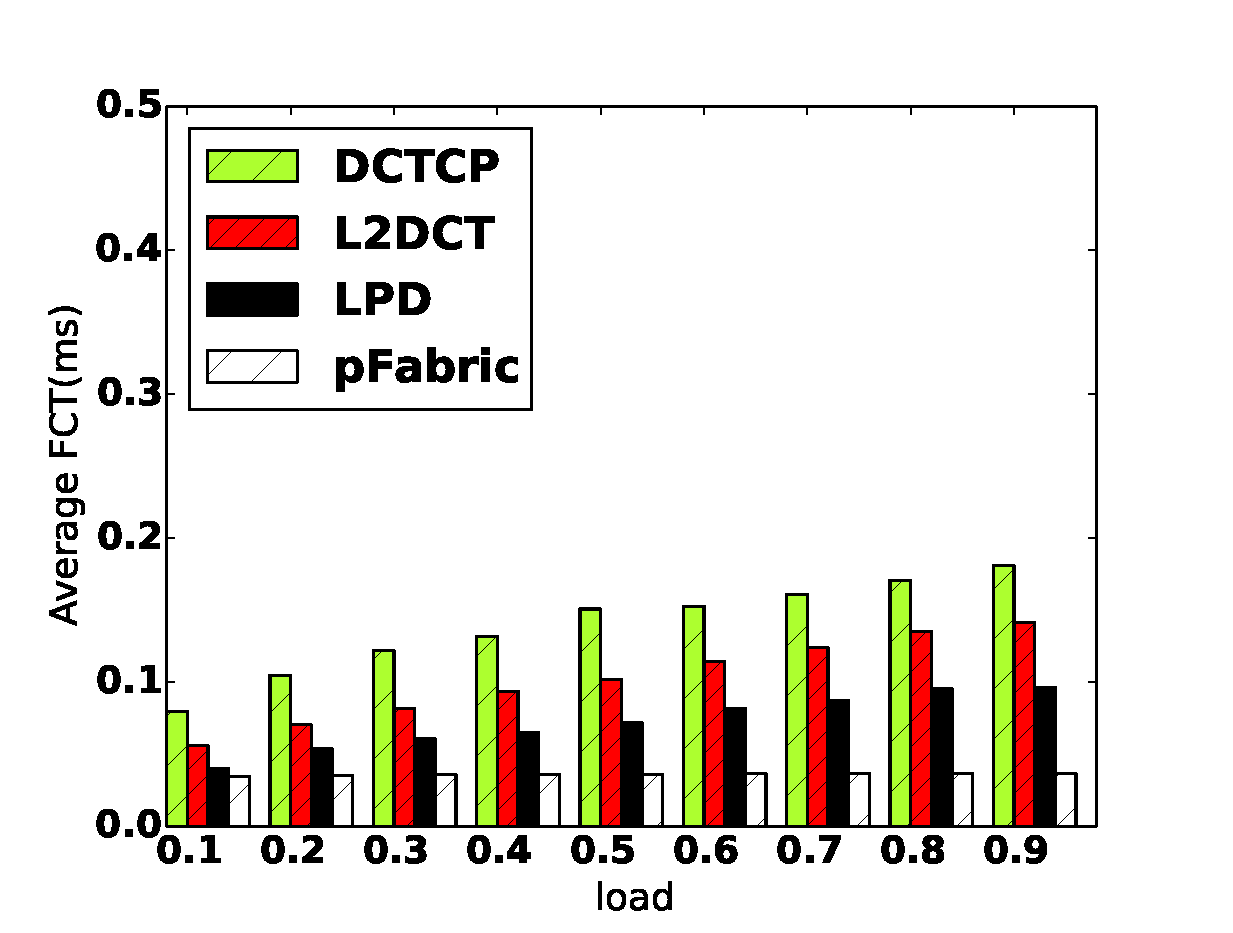
\includegraphics[width=0.32\columnwidth]{figures/LPD/spineleaf/FCT_SEARCH_small.eps}}
\caption{网络搜索流量下,LPD, L$^2$DCT ,pFabric 和 DCTCP对流平均完成时间的对比,注意图(c)和图(a),(b)的Y轴的单位不同}
\label{fct-spine-search-5-fig}
\end{figure}


\begin{figure}[h]
\centering
\subcaptionbox{流平均完成时间}
 {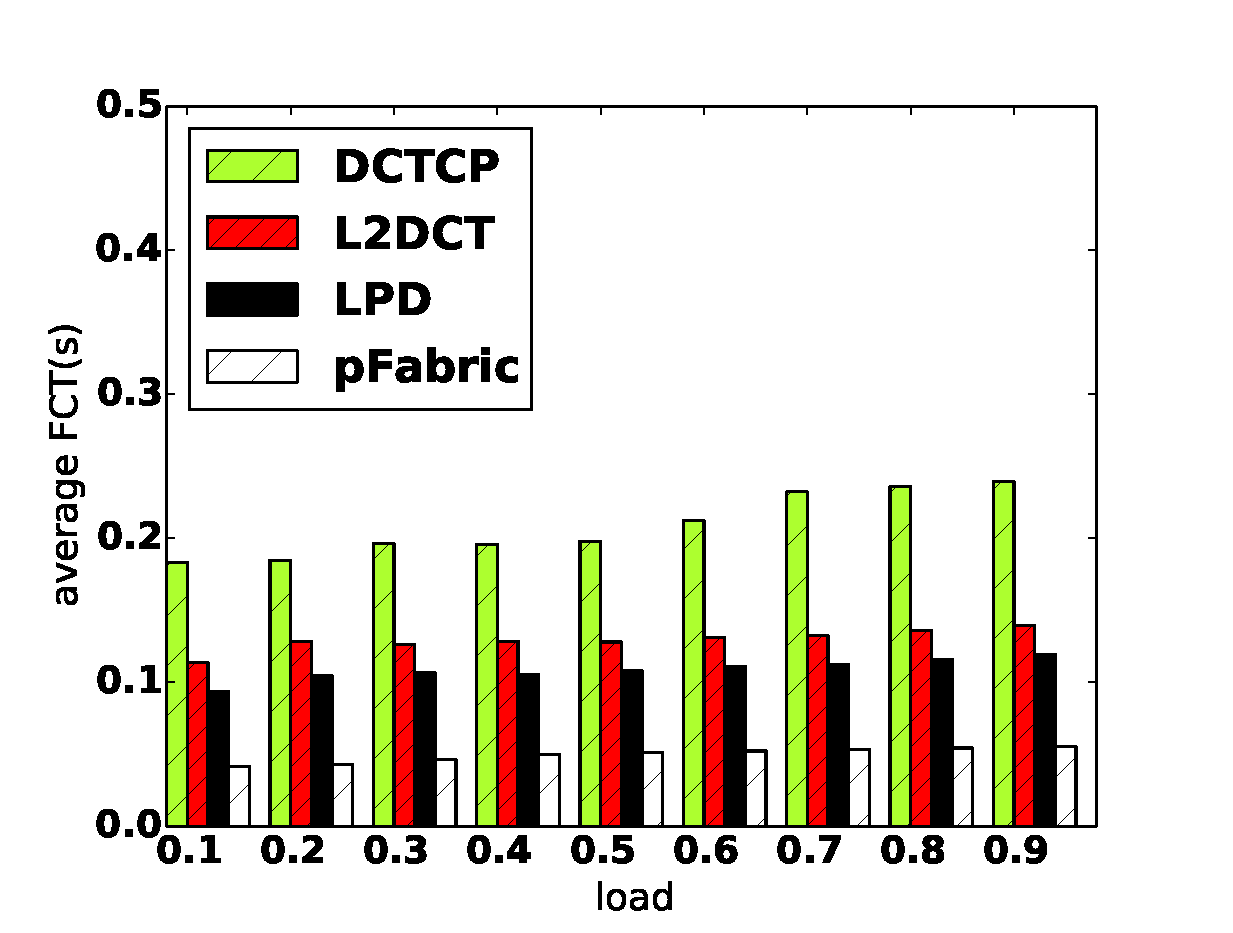
\includegraphics[width=0.32\columnwidth]{figures/LPD/spineleaf/FCT_DATA_average.eps}}
\subcaptionbox{(500KB,+$\infty$)}
{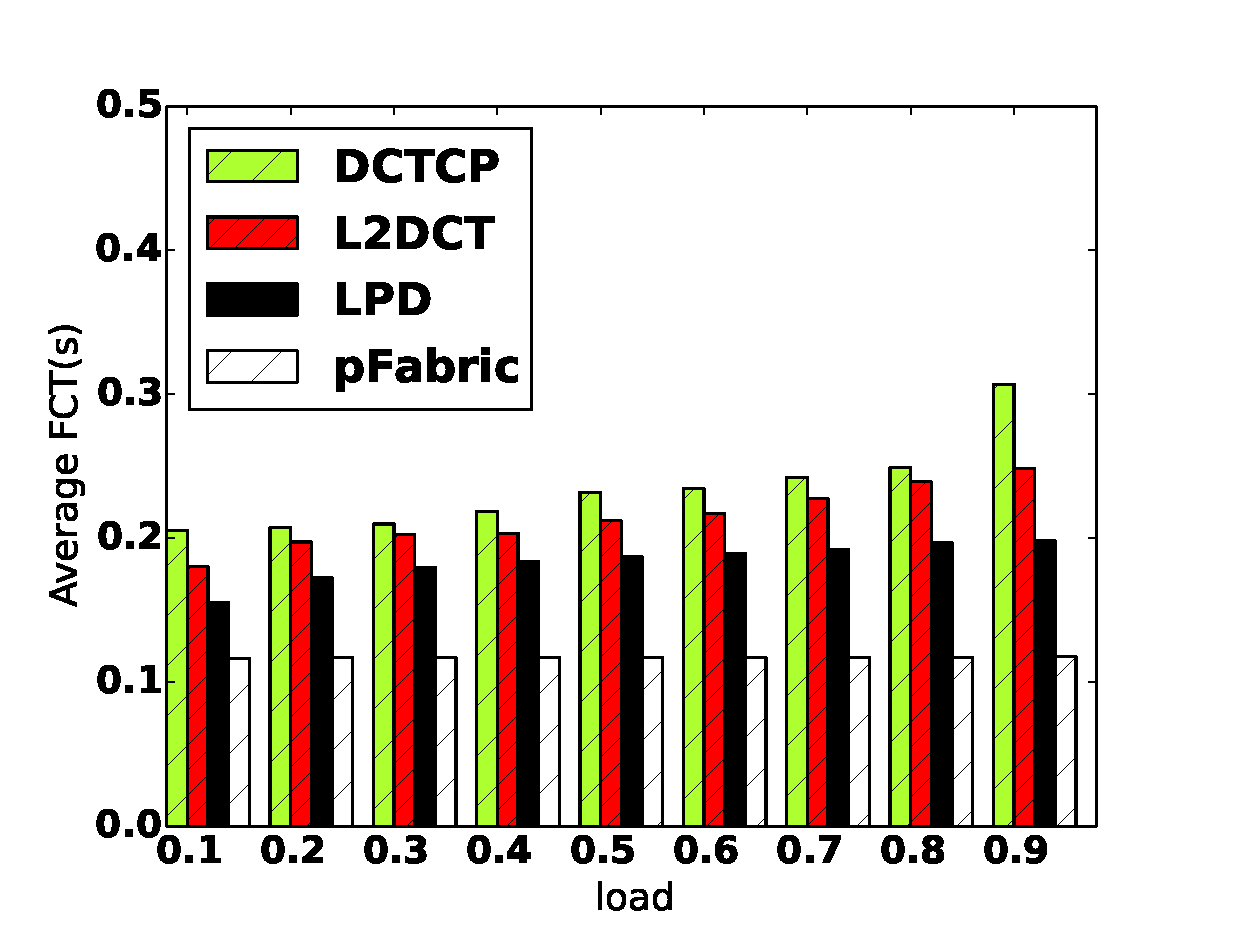
\includegraphics[width=0.32\columnwidth]{figures/LPD/spineleaf/FCT_DATA_large.eps}}
\subcaptionbox{(0,100KB)}
{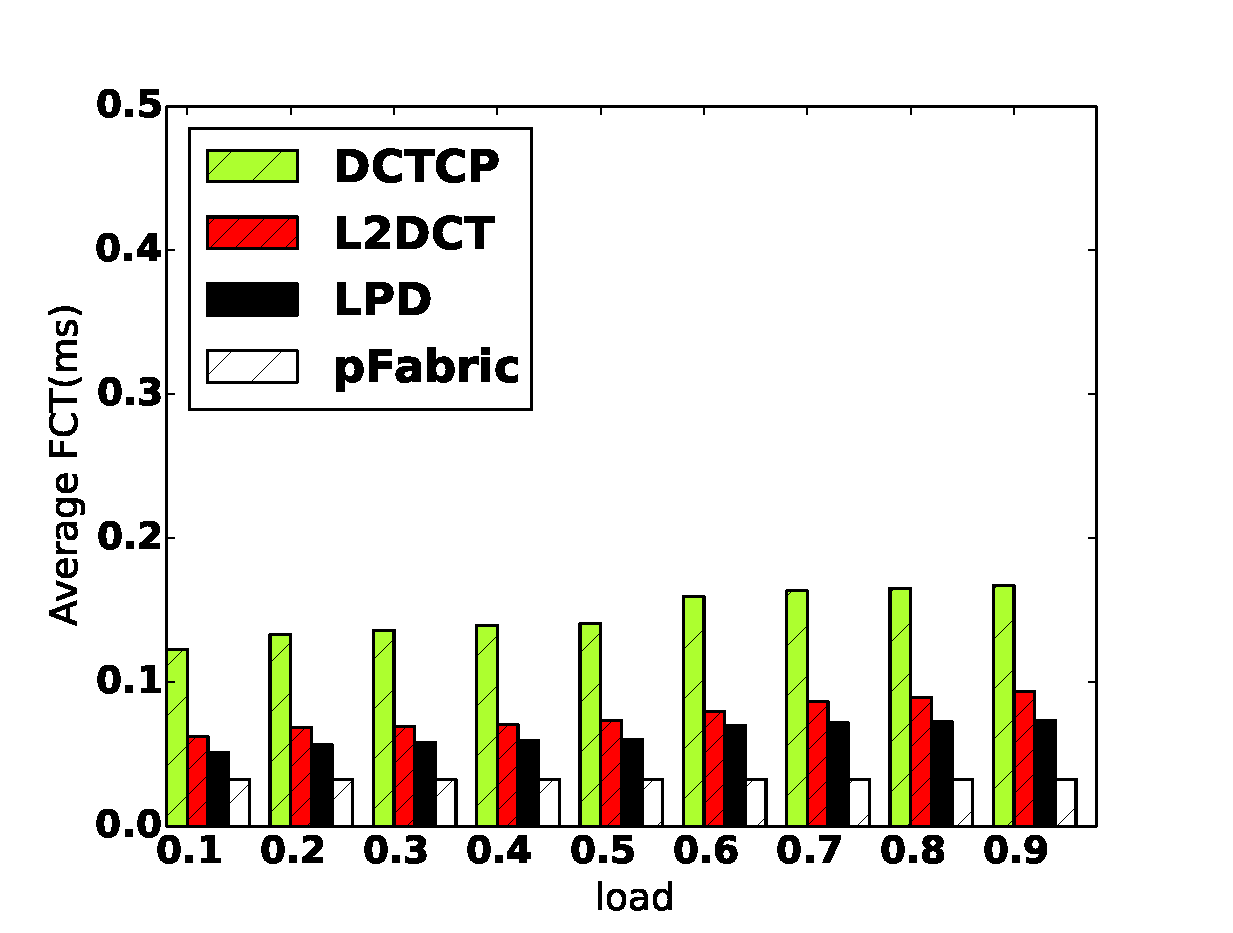
\includegraphics[width=0.32\columnwidth]{figures/LPD/spineleaf/FCT_DATA_small.eps}}
\caption{数据挖掘流量下,LPD, L$^2$DCT ,pFabric 和 DCTCP对流平均完成时间的对比,注意图(c)和图(a),(b)的Y轴的单位不同}
\label{fct-spine-data-5-fig}
\end{figure}


\begin{figure}[h]
\centering
\subcaptionbox{流平均完成时间}
 {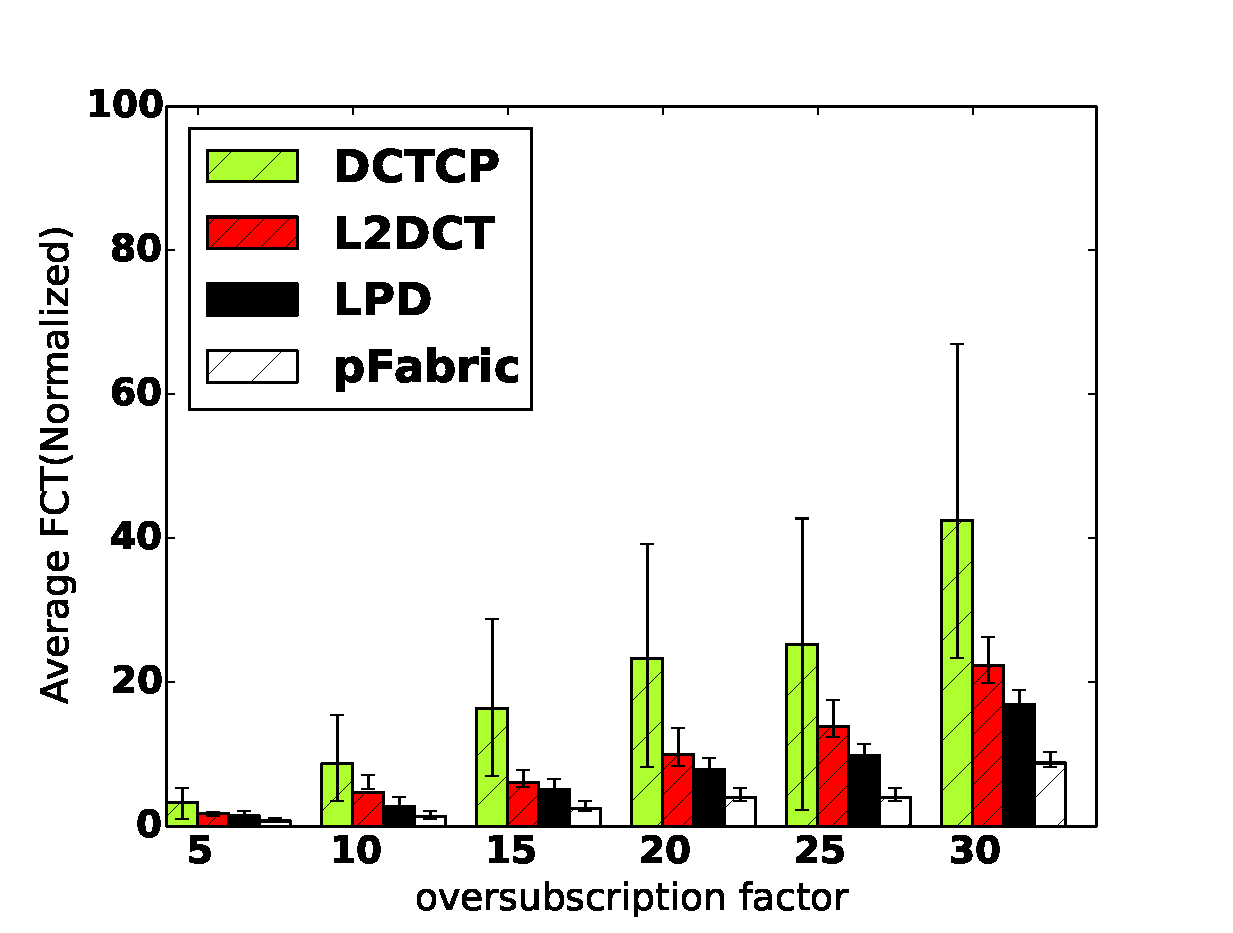
\includegraphics[width=0.32\columnwidth]{figures/LPD/spineleaf/average_fct.eps}}
\subcaptionbox{(500KB,+$\infty$)}
{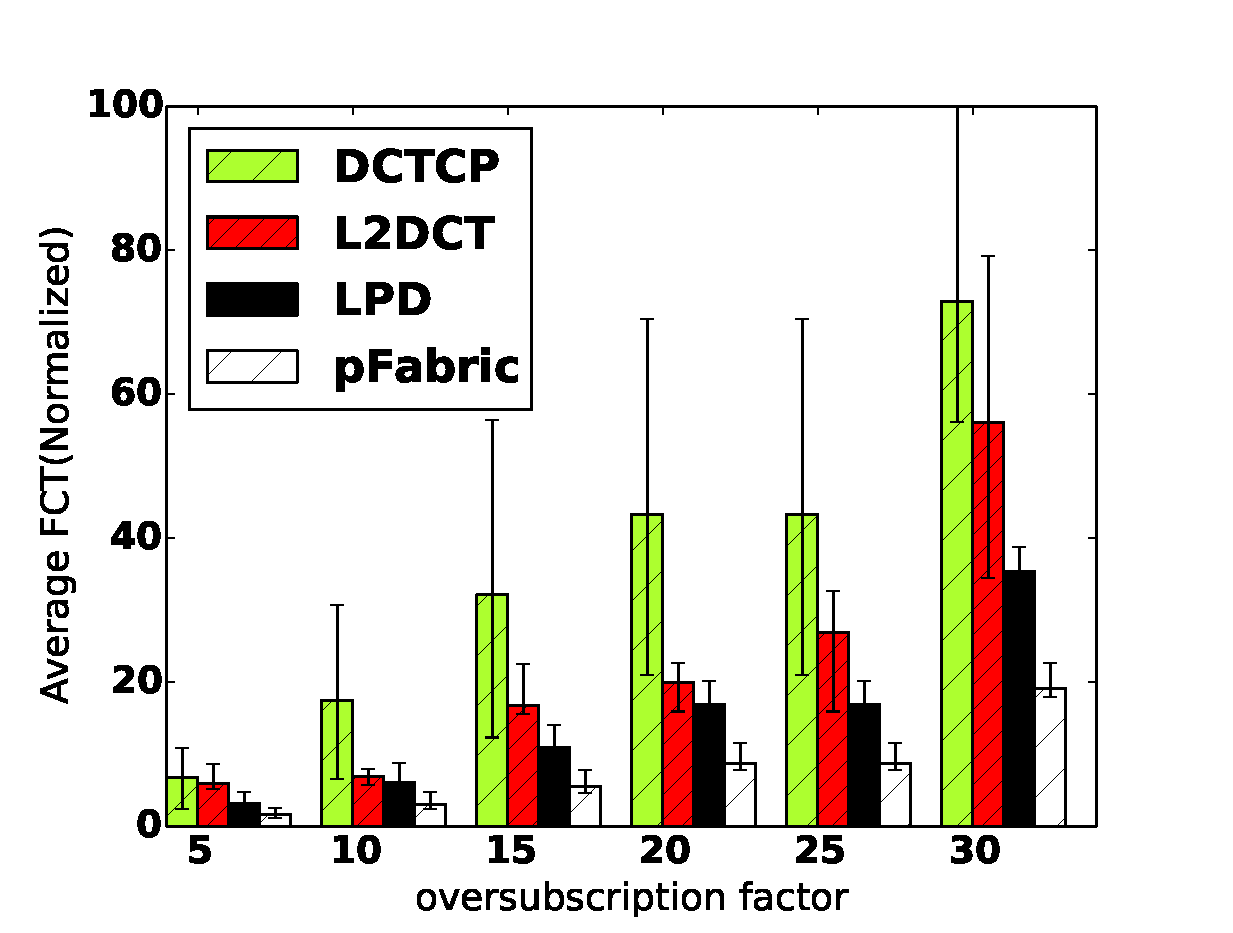
\includegraphics[width=0.32\columnwidth]{figures/LPD/spineleaf/large_fct.eps}}
\subcaptionbox{(0,100KB)}
{\includegraphics[width=0.32\columnwidth]{figures/LPD/spineleaf/small_fct.eps}}
\caption{网络搜索流量下,LPD, L$^2$DCT ,pFabric 和 DCTCP对流平均完成时间的对比,变幻超额认购参数从5到30}
\label{fct-spine-fct-factor-fig}
\end{figure}


“越拥塞,越区分”的原则也可以用于其他目标的优化,比如流平均完成时间(Average Flow Completion Time,简称AFCT)。
改动LPD,并且设置惩罚函数为$f = s / s_{max}$,我们可以得到优化流平均完成时间的策略LPD-s。
在LPD-s中,s可以是流大小或剩余流大小。
在后续实验中,默认s为流大小,并设置$s_{max} = 1MB$。
对于大于1 MB的流,设置其s = 1MB。
对于小于10KB的流,设置s=10KB。
假设N = 1,根据(\ref{tmax}),
LPD-s的流大小调整区域是[10KB,1MB]。
设置超额订购因子x = 5,图\ref{fct-spine-search-5-fig}显示了网络搜索应用下的流平均完成时间结果。


从图\ref{fct-spine-search-5-fig}可以看出,LPD-s和L$^2$DCT均比DCTCP的平均流完成时间都小,但性能不如pFabric。
图\ref{fct-spine-search-5-fig}(a)表明,对于网络负载较轻的场景(load<0.5),LPD-s的性能是DCTCP的3$\times$,大约是L$^2$DCT的$10\%$。
但当网络拥塞很重(load> 0.5)时,LPD-s性能分别比DCTCP和L$^2$DCT提高5$\times$和15$\%$。
图\ref{fct-spine-search-5-fig}(b)显示的是流大小大于500 KB的实验结果。
图\ref{fct-spine-search-5-fig}(c)是小流的结果,注意到图\ref{fct-spine-search-5-fig}(c)与图\ref{fct-spine-search-5-fig}(b)和(a)的y轴有不同的单位。


图\ref{fct-spine-data-5-fig}显示的是数据挖掘流量下流平均完成时间对比。
特别地,从图\ref{fct-spine-data-5-fig}(b)可以看出,LPD下流平均完成时间减小约$40\%$,
而图\ref{fct-spine-search-5-fig}(b)显示了对于长流,LPD在流平均完成时间方面性能提高1$\times$。
对于数据挖掘应用,因为大部分数据流长度大于1MB,因此在实验中,设置$s_{max }$= 1MB,
大于1MB的流被认为有最低优先级,
因而长流的优先级低。

为了测试LPD在网络负载很重的情况下的性能,我们将超额认购因子从5改变到30。
对于每组实验,将网络负载从0.1改变到0.9,图\ref{fct-spine-fct-factor-fig}显示了平均流完成时间和流完成时间的最大值以及每组的最小值。
可以观察到超额认购因子比较小(x= 5)时,LPD的平均流完成时间与L$^2$DCT相比下降了$20\%$。
但是,当网络的超额认购因子较大时,LPD的性能比L$^2$DCT提高1$\times$。
这个结果表明在网络拥塞重的情形下LPD是一个比较好的策略。


\subsection{真实环境下测试}


\begin{figure}[h]
\centering
\subcaptionbox{3条长流带宽}
 {\includegraphics[width=0.45\columnwidth]{figures/LPD/Realtest/realbandwidth2.eps}}
\subcaptionbox{队列长度}
{\includegraphics[width=0.45\columnwidth]{figures/LPD/Realtest/realqueue2.eps}}
\caption{流区分}
\label{real-fig}
\end{figure}


\subsubsection{简单拓扑下的测试}
为了在真实环境下测试LPD的性能,在Linux内核3.2.61中基于DCTCP的代码实现了D$^2$TCP和LPD-e。
交换机使用NetFPGA来实现,并且每个交换机都有4个1Gbps以太网端口,因此数据包可以线速转发和标记。
由于硬件有限,我们只能建立两台交换机和六台服务器的小数据中心拓扑结构。
LPD对Linux内核3.2.61评估的主要代码可以在\cite{LPD-code}下载。


本文首先验证LPD-e是否可以在真实环境中区分不同期限的流量,
流大小设置为10,30和50 MB,相应的截止时间为300,600和900 ms。
图\ref{real-fig}绘制了每个流的带宽随时间的变化情形,以及交换机上的队列长度。
与仿真结果类似,不同截止期限的流程明显不同,队列长度保持在37.5 KB的标记阈值(约为K = 25个1.5 KB的数据包)。

\begin{figure}[H] 
  \centering
  \includegraphics[width=0.7\columnwidth]{figures/LPD/realtopology.pdf}
  \caption{小型数据中心测试床}
\label{testbed-fig}
\end{figure}


\begin{figure}[h]
\centering
\subcaptionbox{随机目的}
 {\includegraphics[width=0.45\columnwidth]{figures/LPD/Realtest/miss_deadline_1.eps}}
\subcaptionbox{OLDI}
{\includegraphics[width=0.45\columnwidth]{figures/LPD/Realtest/miss_deadline_2.eps}}
\caption{LPD 和 DCTCP, D$^2$TCP错失期限对比}
\label{testbed-deadlinemiss-fig}
\end{figure}




\begin{figure}[h]
\centering
\subcaptionbox{随机目的}
 {\includegraphics[width=0.45\columnwidth]{figures/LPD/Realtest/fct_1.eps}}
\subcaptionbox{OLDI}
{\includegraphics[width=0.45\columnwidth]{figures/LPD/Realtest/fct_2.eps}}
\caption{LPD 和 DCTCP,L$^2$DCT流完成时间对比}
\label{testbed-fct-fig}
\end{figure}

\begin{figure}[h]
\centering
\subcaptionbox{OLDI}
 {\includegraphics[width=0.45\columnwidth]{figures/LPD/evaluation_3/lpd.eps}}
\subcaptionbox{网络搜索流量}
{\includegraphics[width=0.45\columnwidth]{figures/LPD/discussion/diss_miss_deadline_.eps}}
\caption{设计原则的进一步拓展}
\label{discussion-fig}
\end{figure}


\begin{figure}[h]
\centering
\subcaptionbox{紧急期限 (20ms)}
 {\includegraphics[width=0.32\columnwidth]{figures/LPD/discussion/20ms.eps}}
\subcaptionbox{中等期限 (30ms)}
{\includegraphics[width=0.32\columnwidth]{figures/LPD/discussion/30ms.eps}}
\subcaptionbox{松弛期限(40ms)}
{\includegraphics[width=0.32\columnwidth]{figures/LPD/discussion/40ms.eps}}
\caption{LPD-r和LPD-e下,OLDI应用期限错失对比}
\label{discussion-r-fig}
\end{figure}


\begin{figure}[h]
\centering
\subcaptionbox{网络搜索流量}
 {\includegraphics[width=0.45\columnwidth]{figures/LPD/discussion/web_search.eps}}
\subcaptionbox{数据挖掘流量}
{\includegraphics[width=0.45\columnwidth]{figures/LPD/discussion/data_mining.eps}}
\caption{LPD-r和LPD-e的下的网络搜索和数据挖掘流量下错失期限对比,流截止期限在10ms到30ms之间,超额认购因子为10}
\label{discussion-r2-fig}
\end{figure}



\subsubsection{小型数据中心测试}
建立一个小型的基于树的测试环境来测试LPD的性能。
图\ref{testbed-fig}显示了拓扑结构。
在此拓扑结构下,两台Linux服务器运行Ubuntu14.04以及dummynet \cite{dummynet,MPTCP} 来构建一个双向瓶颈链路。
修补dummynet用来标记数据包。
在实验中,拓扑中所有接口都是1Gbps。


LPD的惩罚函数遵循“越拥塞,越区分”的原则,即使在网络重度拥塞的的条件下也能区分期限不同的数据流。
因此更多的流能够在最后截止期限前完成。
在实验中,每个服务器$S_i$随机与服务器$S_j$(i$\neq$j)建立连接。
随后$S_i$连续发送数据流给$S_j$。
然后记录数据流错失期限的平均值,最大值和最小值。
图\ref{testbed-deadlinemiss-fig}(a)显示的结果。
可以看到LPD比D$^2$TCP和DCTCP更好。
与DCTCP和D$^2$TCP相比,LPD下流错失期限的比例减少了约$50\%$和$30\%$。
为了观察在OLDI应用下LPD的性能,让$S_1\sim S_6$连续向根R节点发送随机截止期限($\le$10ms)的小流,
图\ref{testbed-deadlinemiss-fig}(b)显示了结果。
可以观察到,LPD比DCTCP性能提高约$30\%$,比D$^2$TCP提高大约$20\%$。
为了测试LPD在减少流完成时间方面的性能,让每个服务器$S_i$将流发送到随机目的节点,
流发送过程持续2分钟,重复这个过程20次,图\ref{testbed-fct-fig}(a)显示了实验结果。
可以看到,与DCTCP和L$^2$DCT相比,LPD流平均完成时间减少了约$20\%$和$10\%$。
随后测试LPD在Partitions-Aggregate的性能,
首先让根节点服务器R向每个端节点发送查询请求,
在端节点接收到查询请求后,它将发送流大小为K的响应数据流。
将K从50 KB变为200 KB,图\ref{testbed-fct-fig}(b)显示实验结果。
可以看到,与DCTCP和L$^2$DCT相比,LPD-s使流平均完成时间分别减少$20\%$和$10\%$。
这是因为LPD采用具有“越拥塞,越区分”的惩罚函数,因此端节点的拥塞控制机制在负载很重的情形下依然有效。

\section{对“越拥塞,越区分”原则的讨论}
 “越拥塞,越区分”这个原则是具有通用性的,本文的策略使用的控制形式:
\begin{equation}
w=
\begin{cases}
w+(1-f) &\text{没有拥塞;}\\
w \times (1-f) &\text{发生拥塞}
\end{cases}\nonumber
\end{equation}
本部分,使用不同的惩罚函数来测试“越拥塞,越区分”原则的通用性。
\subsection{不同的惩罚函数}
设f=a/d,其中d是在D$^2$TCP中使用的期限因子,使用f=a/d作为惩罚函数,
把这个策略成为LPD-d。
LPD-d已经用来解决研究动机提出的问题。
此外,引入另一种拥塞控制机制:
$$ f=\left\{
\begin{array}{rcl}
(2-d)^\alpha      &      & {0      <d      <1}\\
\alpha    &      & {d=1}\\
\alpha*\frac{2-d}{2d-\alpha}     &      & {d>1}\\
\end{array} \right. $$
可以证明$\frac{\partial{(1-f)}}{\partial{d}}>0$, 此外$\frac{\partial^{2}{(1-f)}}{\partial{\alpha}\partial{d}}>0$,
此例符合本文提出的“越拥塞,越区分”的原则,称之为MLD。


设置流的期限满足统一分布,图\ref{discussion-fig}(a) 描述了OLDI应用下LPD-e, MLD 和 LPD-d性能对比。
图\ref{discussion-fig}(b)下网络搜索流量下的结果。
图\ref{discussion-fig}显示不同形式的算法的差异性不大,
策略能够在网络拥塞程度重的情形下使的期限不同的数据流。

\subsection{使用剩余时间}

在\ref{sec_LPD:LPD}节中提出LPD-e,使用流程开始时间和截止期限之间的时间间隔。
因为,减少流错失期限的最优策略是最小期限优先策略。 
使用另一种策略,使用当前时间和截止期限之间的持续时间作为调整因子,称之为LPD-r策略。
 
 
使用的相同参数来评估LPD-r,并将其与LPD-e进行比较。
 图\ref{discussion-r-fig}描绘了在简单拓扑下OLDI应用LPD-r与LPD-e错失期限情形对比。
 而图\ref{discussion-r2-fig}描绘了在spine-leaf拓扑中的在网络搜索和数据挖掘下错失期限对比。
从实验结果中,可以看到LPD-r和LPD-e性能相近,
这再一次证实了“越拥塞,越区分”原理的通用性,
因此在实际中,可以使用不同的惩罚函数以及不同的期限因子设计拥塞控制机制。

\section{本章总结}
\label{sec_LPD:Conclusion}
本章提出“越拥塞,越区分”的原则来设计数据中心拥塞控制机制。
根据本原则设计的拥塞控制机制,使的网络即使在严重拥塞的情形下依然可以根据截止期限分配带宽。
为了证明这个原则的有效性,本文设计了速率控制机制-负载自适应拥塞控制策略(load proportional differentiation,简称LPD),
并使用不同的网络拓扑和网络流量测试LPD的性能。
实验发现LPD的性能几乎超越了例如D$^{2}$TCP, L$^{2}$DCT等当前最先进的拥塞控制机制。

尽管LPD用来使的更多数据流在截止期限之前完成,原则“越拥塞,越区分”是有通用性,
用户可以根据这个原则设计其它的拥塞控制机制。
然而,关于LPD的收敛性和稳定性,在以后的工作中需要进行进一步的讨论。


